\chapter{HiSPARC as a Space Weather Detector}\label{chap:HiSPARC}

%%%%%%%%%%%%%%%%%%%%%%%%%%%%%%%%%%%%%%%%%%%%%%%%%%%%%%%%%%%%%%%%%%%%%
%%%%%%%%%%%%%%%%%%%%%%%%%%%%%%%%%%%%%%%%%%%%%%%%%%%%%%%%%%%%%%%%%%%%%
\section{Introduction}\label{sec:HS_intro}

... [on daily variations (DV)] Dr. Rolf Butikofer (in a reply from Danislav Sapundjiev, dasapund@meteo.be) said:

\textit{"The daily cosmic ray variation near Earth is caused by the anisotropy of the cosmic ray intensity in the interplanetary space. Cosmic ray particles follow the field lines of the interplanetary magnetic field when they travel towards the interior of the heliosphere. Because of the rotation of the Earth, the angle between the asymptotic cone of acceptance of various energies at the location of ground-based cosmic ray detectors (neutron monitors) and the direction of the interplanetary magnetic field varies with a time period of 24 hours. As a consequence cosmic ray detectors look in different directions in the course of a day and observe therefore a diurnal variation. The daily variations of neutron monitors is mainly seen by high latitude stations which have asymptotic directions at low energies (rigidities) near the equator."}


%%%%%%%%%%%%%%%%%%%%%%%%%%%%%%%%%%%%%%%%%%%%%%%%%%%%%%%%%%%%%%%%%%%%%
\subsection{HiSPARC Project}

%%%%%%%%%%%%%%%%%%%%%%%%%%%%%%%%%%%%%%%%%%%%%%%%%%%%%%%%%%%%%%%%%%%%%
\subsection{HiSPARC Detector}
 - design
 
 - scintillators
 
 - typical layouts (i.e. 2d or 4d)
 
 - trigger conditions


%%%%%%%%%%%%%%%%%%%%%%%%%%%%%%%%%%%%%%%%%%%%%%%%%%%%%%%%%%%%%%%%%%%%%
%%%%%%%%%%%%%%%%%%%%%%%%%%%%%%%%%%%%%%%%%%%%%%%%%%%%%%%%%%%%%%%%%%%%%
\section{Aims}\label{sec:HS_aims}
The HiSPARC project was set up with the detection philosophy of observing extended air showers (EAS), which are typically associated with PCRs with energy of $\sim10^{14}$~eV and above, that produce large footprints observable with many HiSPARC stations simultaneously. For PCRs with energy below $\sim10^{14}$~eV the air shower is small, with almost no observable footprint, and for PCRs with energy below $\sim10^{11}$~eV, there are typically less than one or two muons that reach the ground, making their observation difficult. 

The HiSPARC detectors are capable of observing any muons that reach them, therefore the project was motivated by the existing network of muon detectors which may have the capability of observing the cosmic rays associated with space weather events.

The principle aim of the project was to determine whether the existing HiSPARC network is capable of observing space weather events. This was initially achieved by investigating the data during periods of space weather activity to search for the associated signatures. In addition, simulations of air showers initiated by CRs were conducted to understand the expected muon flux at ground level.


%%%%%%%%%%%%%%%%%%%%%%%%%%%%%%%%%%%%%%%%%%%%%%%%%%%%%%%%%%%%%%%%%%%%%
%%%%%%%%%%%%%%%%%%%%%%%%%%%%%%%%%%%%%%%%%%%%%%%%%%%%%%%%%%%%%%%%%%%%%
\section{HiSPARC Properties}\label{sec:HS_properties}
 - Selected HS stations
 - Locations of stations
 - PLANETOCOSMICS simulations (explain)
 - Rigidities
 - Asymptotic viewing directions
 

To understand the PCR spectrum that the HiSPARC stations are capable of observing, PCR transport simulations were performed using the PLANETOCOSMICS software. PLANETOCOSMICS performs Geant4 Monte Carlo simulations of charged particle transport through Earth's magnetosphere based on St\o rmers transport equation for charged particles \citep{desorgher_planetocosmics_2006}. PLANETOCOSMICS simulates backward trajectories of charged particles from a given location (latitude, longitude, and altitude) out to the magnetopause for a set of PCR rigidites. 

For each trajectory there are two possible outcomes: (i) the particles trace out to the magnetopause where they escape Earth's magnetosphere, an allowed trajectory; (ii) the particles are sufficiently bent by the effect of the Earth's magnetosphere that they do not reach the magnetopause and cannot escape the Earth's magnetosphere, a forbidden trajectory \citep{desorgher_planetocosmics_2006}. The coordinates of the asymptotic direction at the magnetosphere are provided as an output to the simluations projected back down to the Earth's surface. In this work PLANETOCOSMICS was configured with the Tsyganenko-89 model for the external magnetospheric magnetic field and the IGRF internal field model.

For each rigidity simulated, whether it was an allowed or forbidden trajectory was stored, which was used to provide an insight into the rigidity spectrum for a given station. From the allowed trajectories the effective cut-off rigidity ($R_C$) for the stations was computed using equation~(\ref{eq:cut_off}), where $R_U$ is the upper rigidity (the last allowed trajectory before the first forbidden trajectory); $R_L$ is the lower rigidity (the last allowed trajectory before which all other trajectories with a lower rigidity are forbidden); $\Delta R$ is the rigidity step size in the simulation \citep{desorgher_planetocosmics_2006, herbst_influence_2013}.

\begin{equation}
\label{eq:cut_off}
R_C = R_U - \sum_{i = R_L}^{R_U} \Delta R_i
\end{equation}

The rigidity spectrum for each of the HiSPARC stations were investigated to determine $R_C$ for each station. The cut-off rigidity calculated for the six HiSPARC stations for a vertical incidence upon the atmosphere (i.e. $0^\circ$ zenith angle) are shown in Table~\ref{tab:HS_stns} which show that there is little variation in $R_C$ between the HiSPARC stations and that they observe protons with rigidities in excess of $\sim 3$ GV. This analysis was initially carried out for the vertical direction (i.e. azimuth = $0^\circ$, zenith = $0^\circ$); however further trajectories were simulated for different azimuth and zenith angles to determine the dependence of the rigidity spectrum on the detector acceptance angle. The analysis for the azimuthal dependence was carried out at a zenith angle of $20^\circ$ as this is around the most probably angle for HiSPARC events, and the analysis of the zenith dependence was carried out at an azimuth angle of $0^\circ$.


\begin{table}
	\begin{center}
		\caption{Properties of some of the HiSPARC stations: geographic longitude ($\lambda$), geographic latitude ($\phi$), altitude ($h$), and the geomagnetic vertical cut-off rigidity ($R_C$) calculated from the PLANETOCOSMICS simulations.}
		\label{tab:HS_stns}
		\begin{tabular}{l c c c c c}
			\hline
			& $R_C$  & $\lambda$ & $\phi$  & $h$  & No. Detectors\\
			Station Name/ID & [GV] & [deg] & [deg] & [m]  & \\
			\hline
			Nikhef/501 & 3.19 & 4.95 E & 52.36 N & 56.18 & 4 \\
			College Hageveld/203 & 3.18 & 4.63 E  & 52.35 N & 53.71  & 2 \\
			Leiden/3001 & 3.23 & 4.45 E & 52.17 N & 54.08 & 2 \\
			Eindhoven/8001  & 3.44 & 5.49 E & 51.45 N & 70.12 & 2 \\
			Birmingham University/14001  & 3.06 & 1.93 W & 52.45 N & 204.14 & 4  \\
			%20003 & 2.30 & 10.20 E & 56.17 N & 84.38 & 2 \\
			\hline
		\end{tabular}
	\end{center}
\end{table}

\begin{figure}[h]
	\centering
	\subfloat[Azimuth variation (fixed zenith = $20^\circ$)]{
		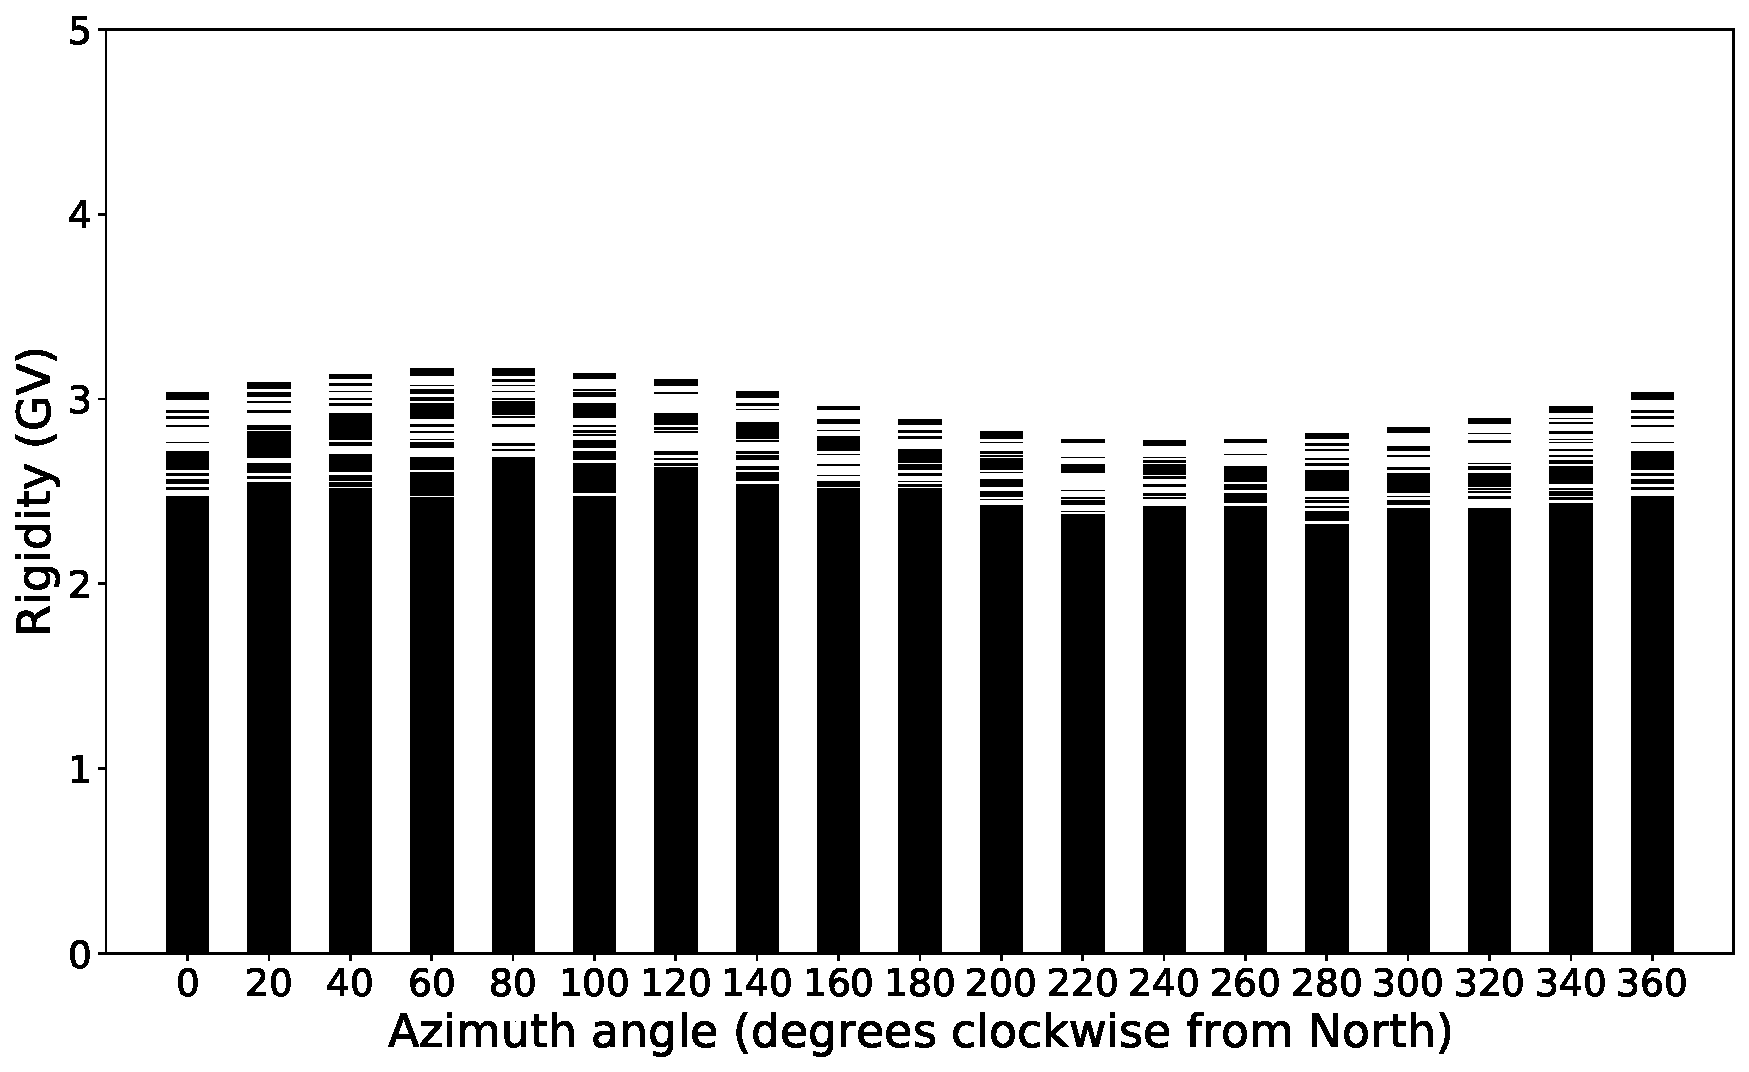
\includegraphics[width=0.48\columnwidth]{azm.pdf}
		\label{fig:azm1}}
	%\qquad
	\subfloat[Zenith variation (fixed azimuth = $0^\circ$)]{
		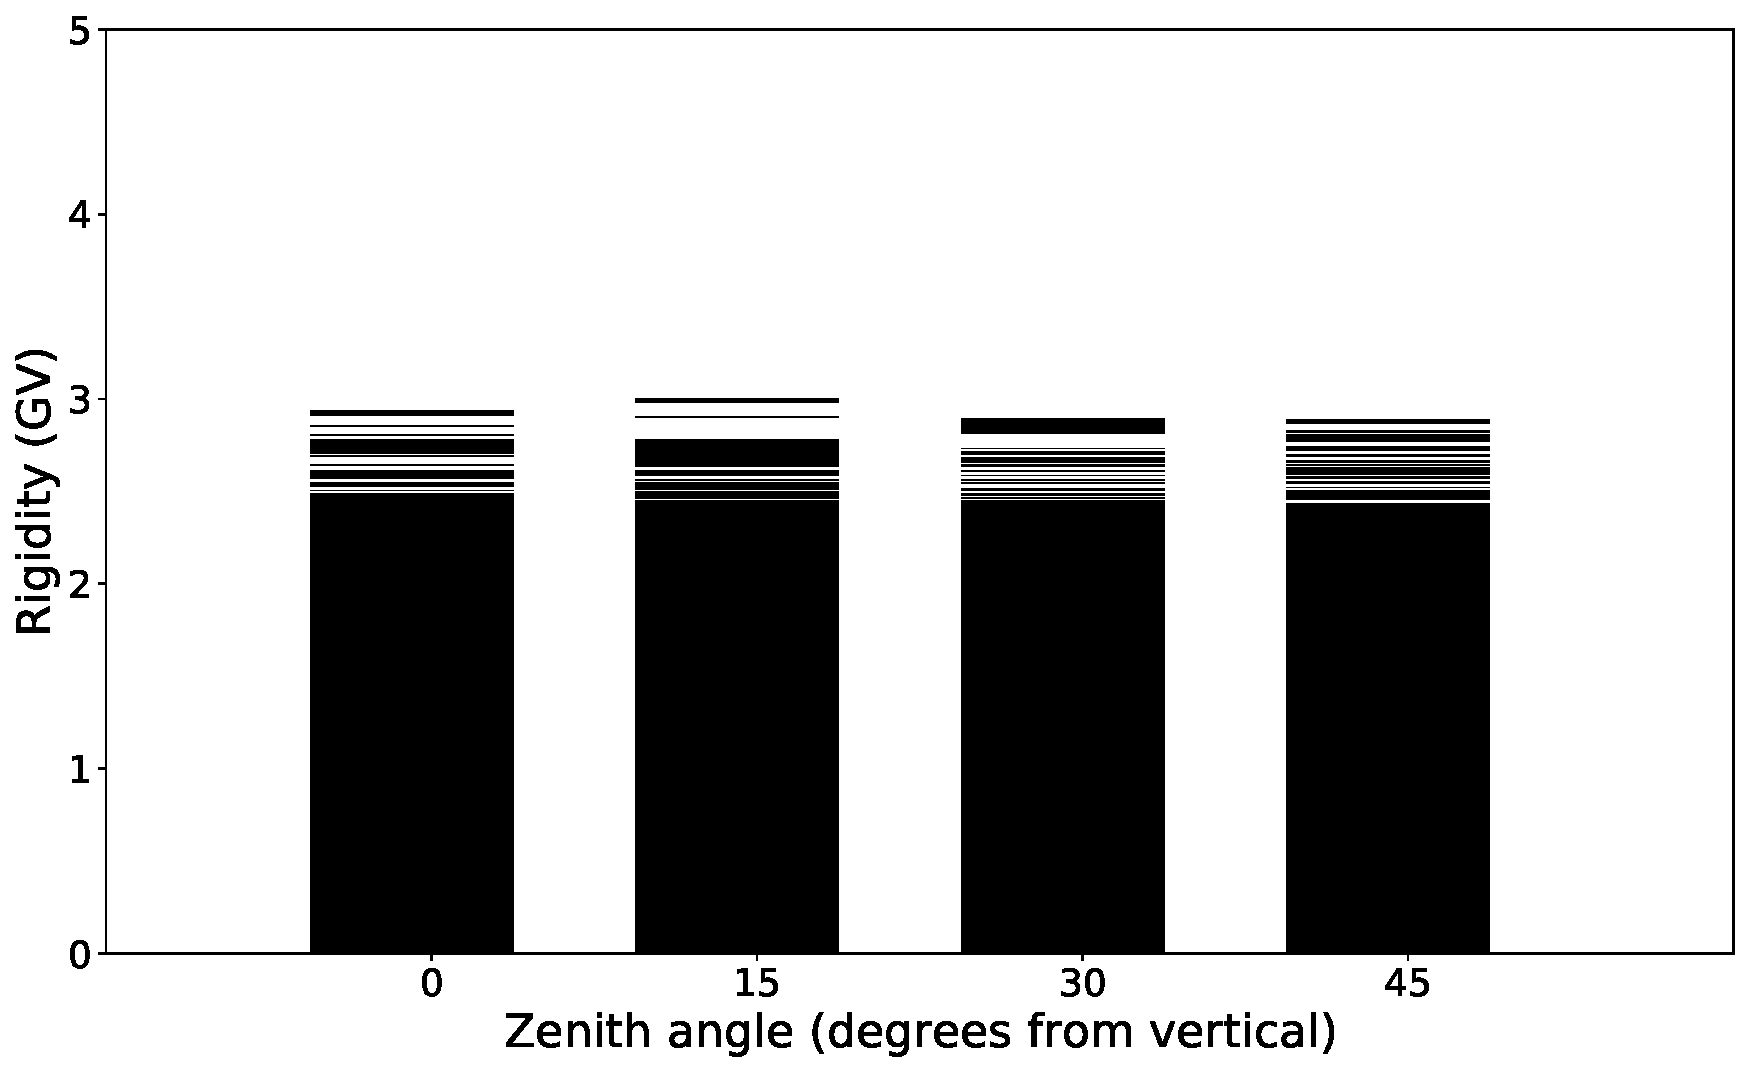
\includegraphics[width=0.48\columnwidth]{zen.pdf}
		\label{fig:zen1}}
	
	\caption{Azimuthal and zenith angle variations in the allowed and forbidden rigidity trajectories for HiSPARC station 501.}
	\label{fig:R_C2}
\end{figure}

The small variation between HiSPARC stations is due to their close proximity in geographic latitude and longitude. The values of $R_C$ calculated for the HiSPARC stations suggest that they should be able to observe higher energy SCRs, but may not be as susceptible as the higher latitude NMs where the effects of GLEs are highly observable.

As a results of the PLANETOCOSMICS simulations it is possible to understand the trajectories of particles that enter the Earth's magnetosphere prior to arrival at the muon detector.

Figre~\ref{fig:HS_AVD}...

\begin{figure}[ht]
	\centering
	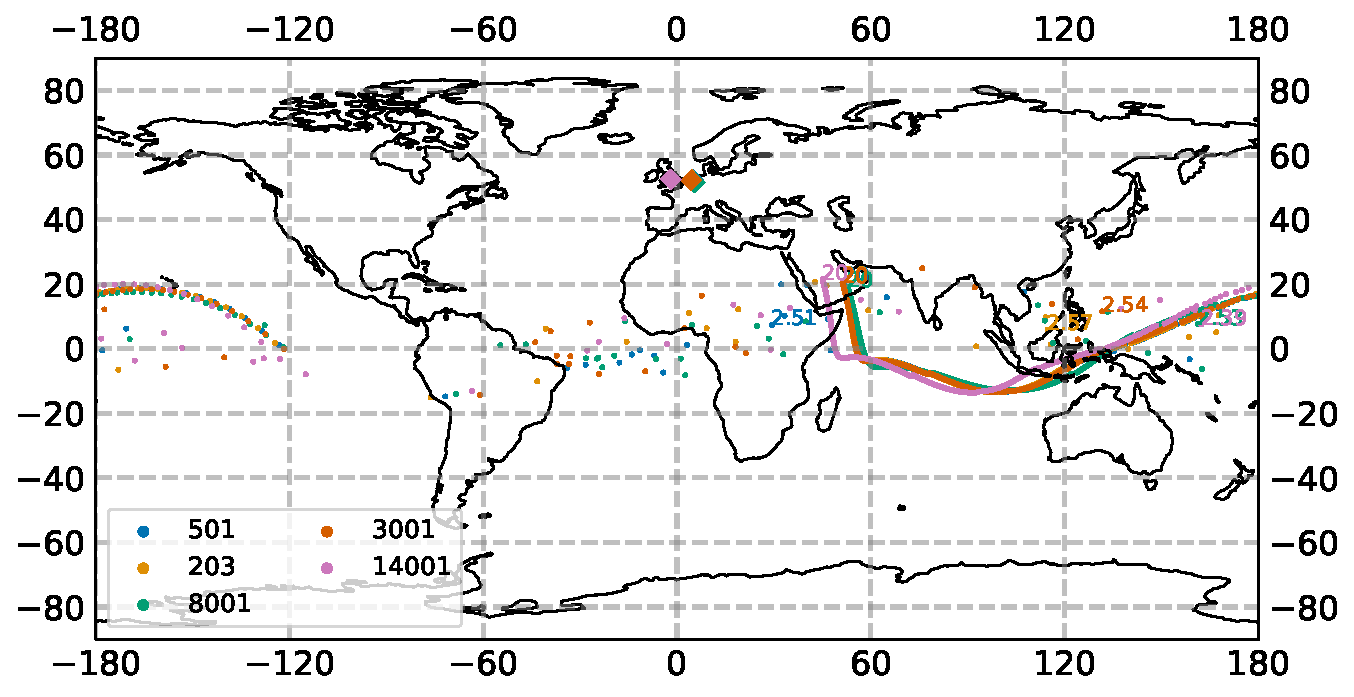
\includegraphics[scale=0.6]{HS_AVDs.pdf}
	\caption{The vertical asymptotic viewing directions of 5 HiSPARC stations. The rigidity range of the simulations were from $1.0$~GV $<$ R $<20.0$~GV, and the results are plotted in geographic coordinates on January 20th 2005. The diamonds correspond to the HS ground location and the circles correspond to the AVD for a specific rigidity value.}
	\label{fig:HS_AVD}
\end{figure}


 

%%%%%%%%%%%%%%%%%%%%%%%%%%%%%%%%%%%%%%%%%%%%%%%%%%%%%%%%%%%%%%%%%%%%%
%%%%%%%%%%%%%%%%%%%%%%%%%%%%%%%%%%%%%%%%%%%%%%%%%%%%%%%%%%%%%%%%%%%%%
\section{HiSPARC Observations}\label{sec:HS_obs}


[discuss preliminary observation of space weather FDs and GLEs for the events and singles data...]

[end with discussion on unknown PCRs observable and the effect of atmospheric weather conditions that need to be accounted for]

The effects of space weather on CRs has been outlined in [REF intro]. It was highlighted during communication with the UK Met Office that observations of GLEs are of more interest and importance to space weather forecasts and nowcasts. FDs are of lower interest and importance, however they were still searched for within the HiSPARC data. The events that were looked for within the HiSPARC data are outlined in Table~\ref{tab:space_weather_events}.

\begin{table}
	\begin{center}
		\caption{Space weather events investigated within the HiSPARC data. The percentage change column provides a reference of how much the CR counts observed by the NM station at Oulu (R$_c$=0.81~GV) increased of decreased by, due to the space weather event.}
		\label{tab:space_weather_events}
		\begin{tabular}{c c c | c c}
		\hline
		{\bf GLE Onset} & {\bf GLE} & {\bf \% Change (Oulu)} & {\bf FD Onset} & {\bf \% Change (Oulu)}\\
		\hline
		{13/12/2006} & {70} & {$\sim 100\%$} & {08/03/2012} & {$\sim 5\%$}  \\
		{17/05/2012} & {71} & {$\sim 15\%$} & {14/07/2012} & {$\sim 3\%$} \\
		{10/09/2017} & {72} & {$\sim 5\%$} & {21/12/2014} & {$\sim 5\%$} \\
		{} & {} & {} & {06/09/2017} & {$\sim 2\%$} \\
		{} & {} & {} & {07/09/2017} & {$\sim 8\%$} \\
		\hline
		\end{tabular}
	\end{center}
\end{table}



%%%%%%%%%%%%%%%%%%%%%%%%%%%%%%%%%%%%%%%%%%%%%%%%%%%%%%%%%%%%%%%%%%%%%
\subsection{HiSPARC Observations of Ground Level Enhancements}

Initial searches for evidence of GLEs within the HiSPARC data were conducted for GLE 70, 71, and 72, as they arethe only GLEs that span the operational epoch of the HiSPARC network.

Figure~\ref{fig:GLE_70}...

\begin{figure}[h]
	\centering
	\subfloat[HS 501 (Nikhef)]{
		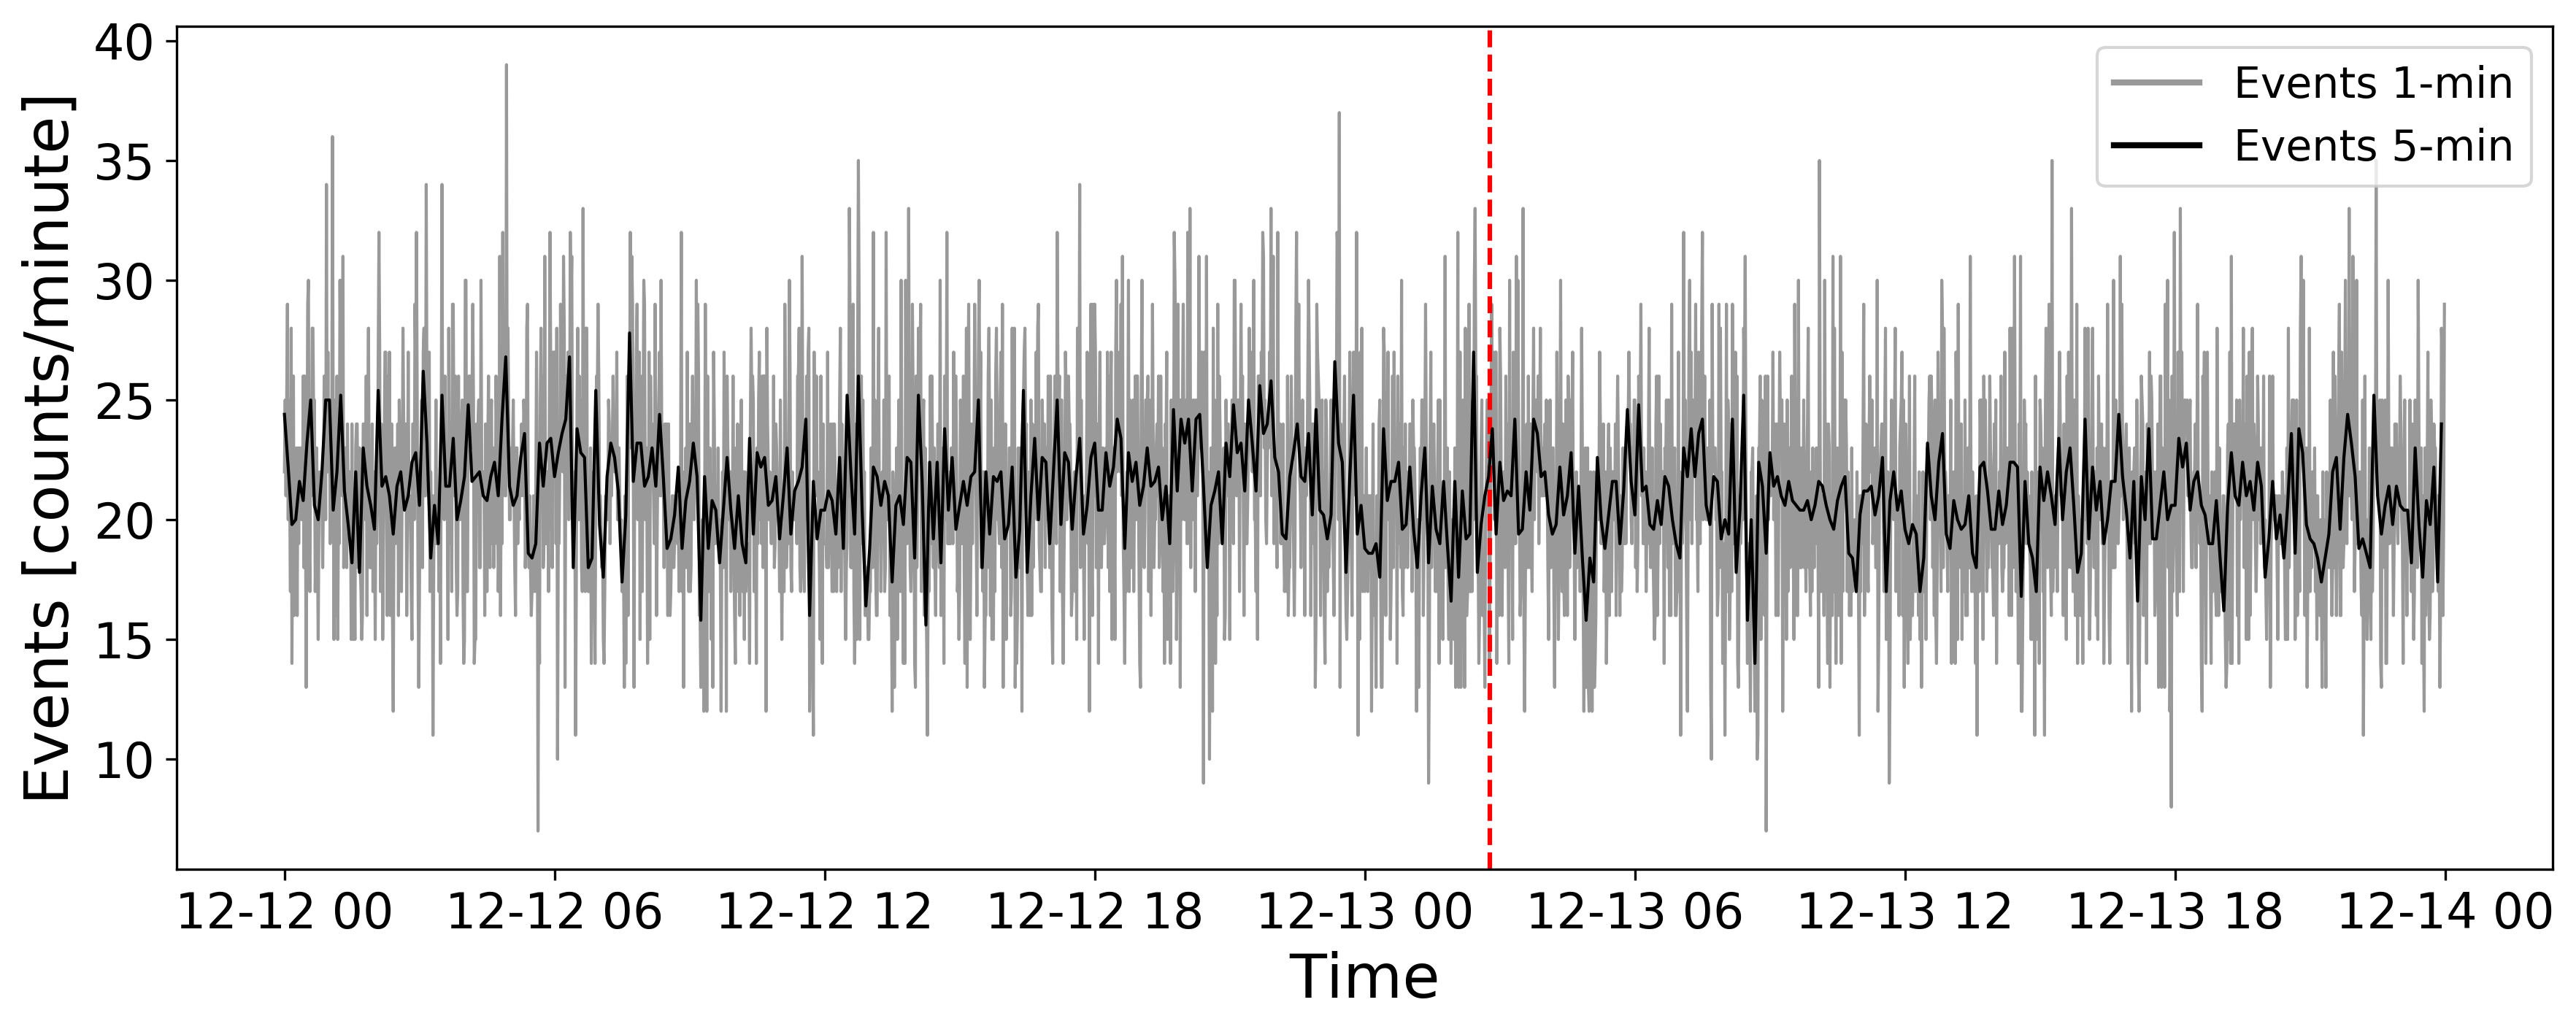
\includegraphics[width=0.48\columnwidth]{GLE70_501.png}
		\label{fig:GLE70_501}}
	%\qquad
	\subfloat[HS 3001 (Universiteit Leiden)]{
		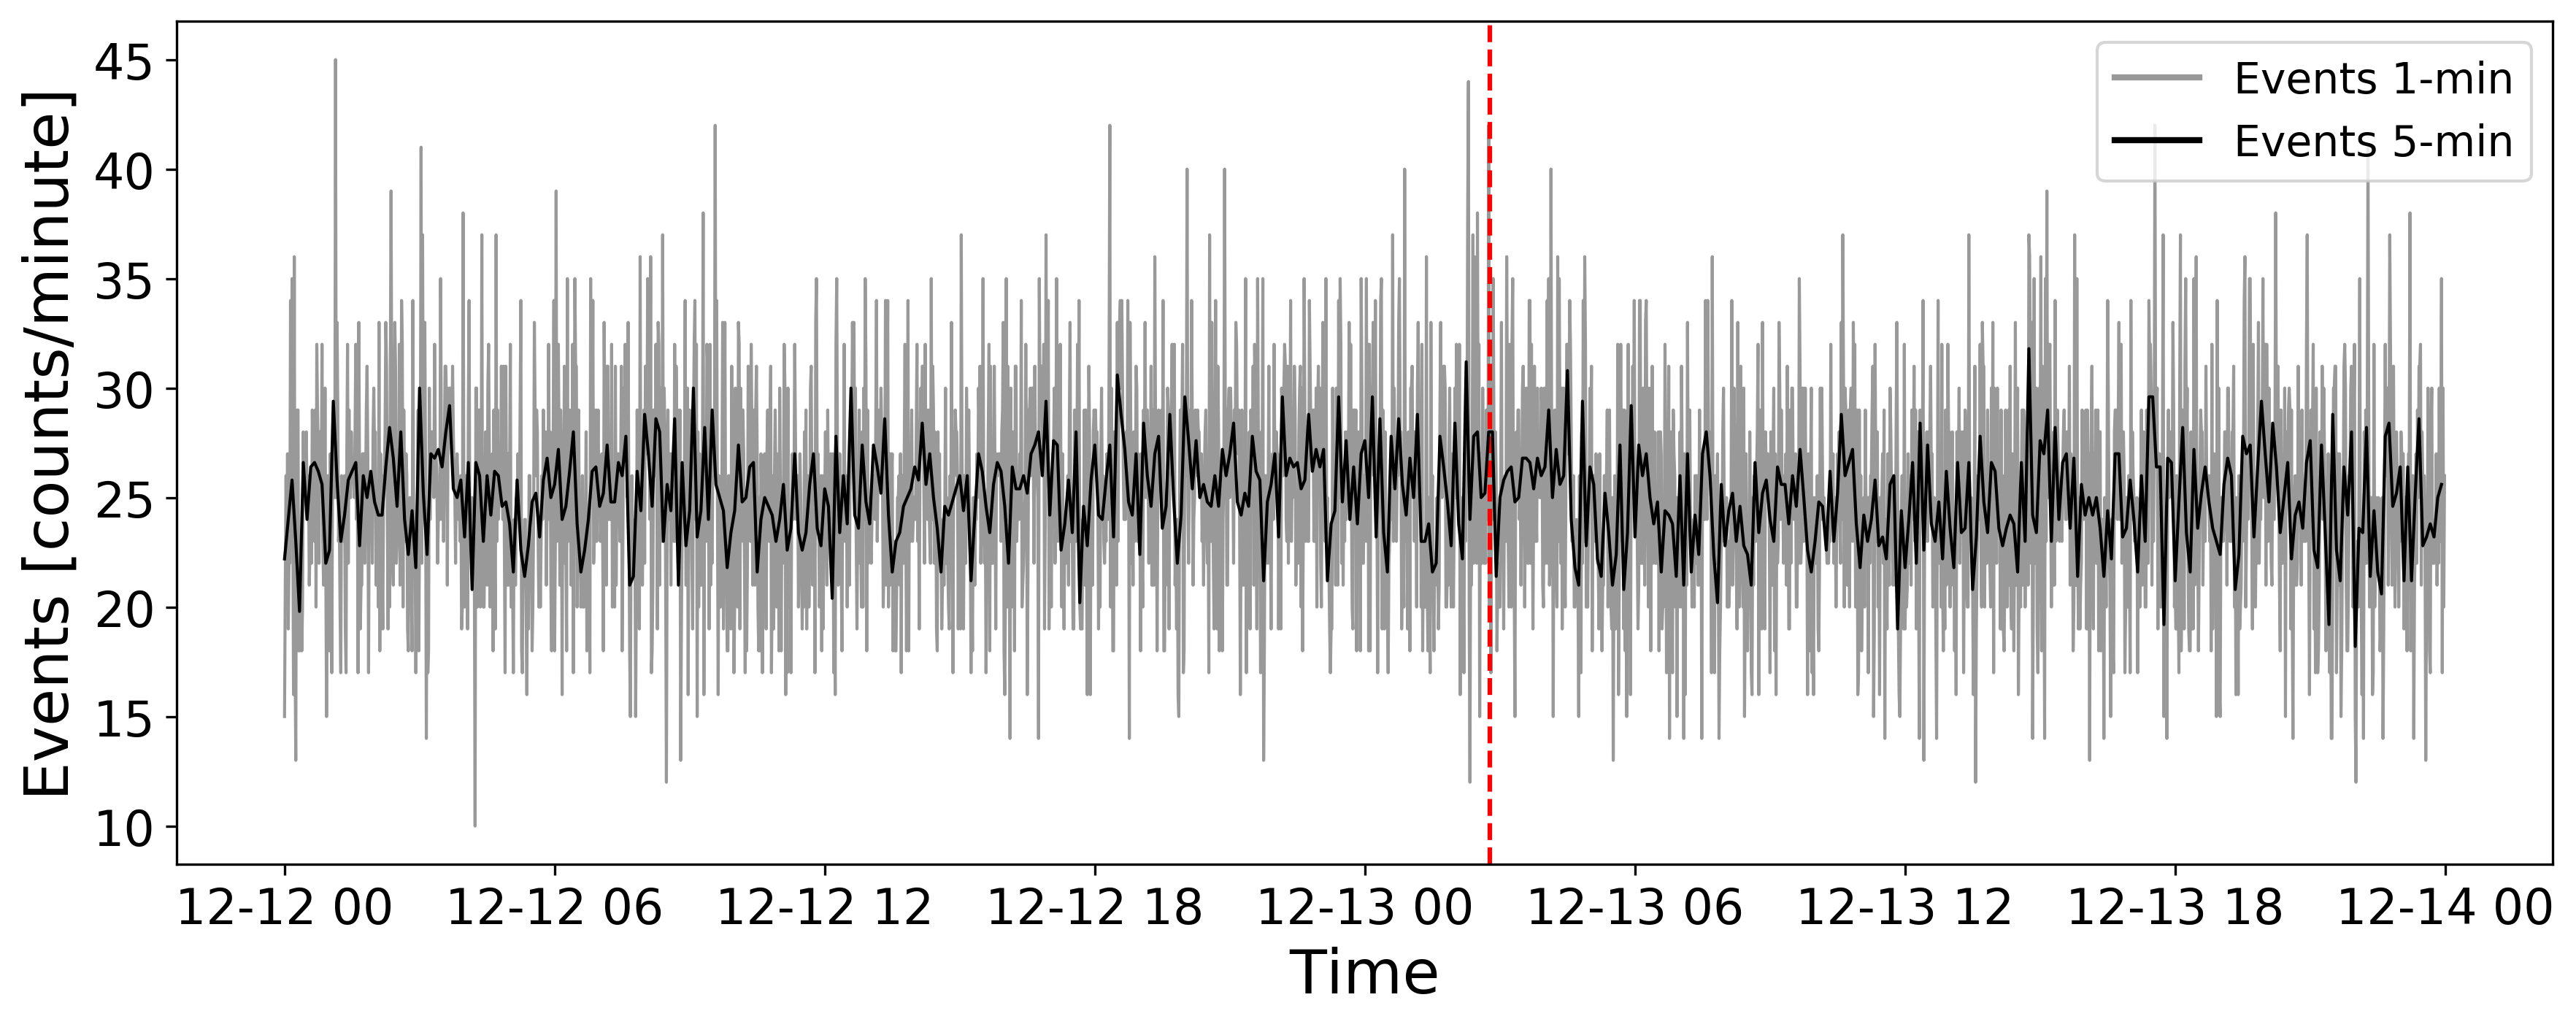
\includegraphics[width=0.48\columnwidth]{GLE70_3001.png}
		\label{fig:GLE70_3001}}
	
	\caption{HiSPARC data for stations 501 and 3001 around the epoch of GLE 70. The plot shows the minute-averaged and 5-minute-averaged trigger events between detectors within the station. The vertical red, dashed line depicts the approximate onset time of the GLE.}
	\label{fig:GLE_70}
\end{figure}


Figure~\ref{fig:GLE_71}...

\begin{figure}[h]
	\centering
	\subfloat[HS 8001 (Eindhoven)]{
		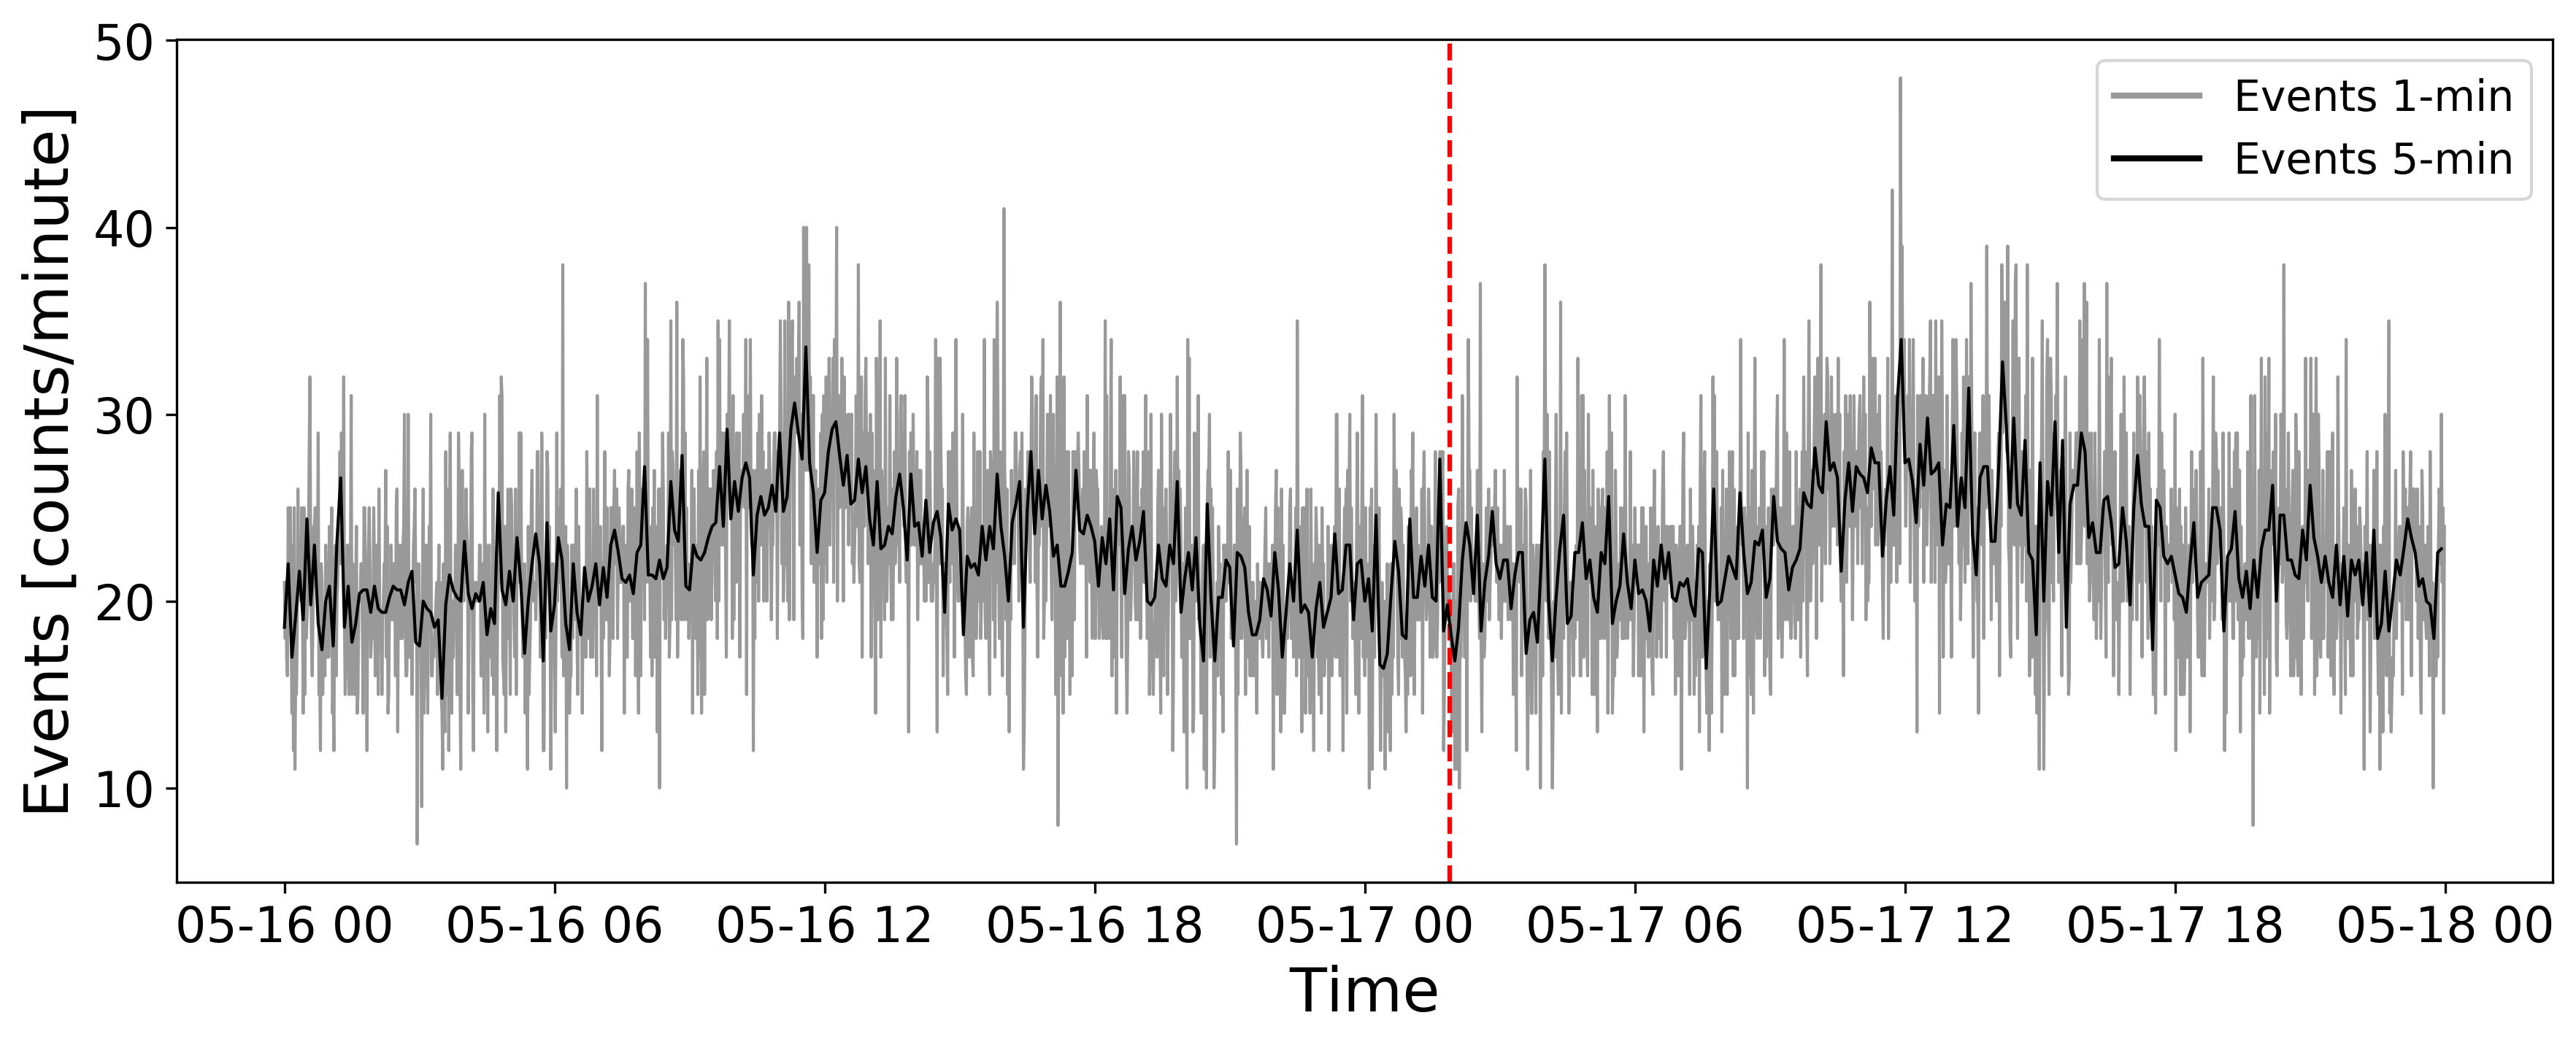
\includegraphics[width=0.48\columnwidth]{GLE71_8001.png}
		\label{fig:GLE71_8001}}
	%\qquad
	\subfloat[HS 3001 (Universiteit Leiden)]{
		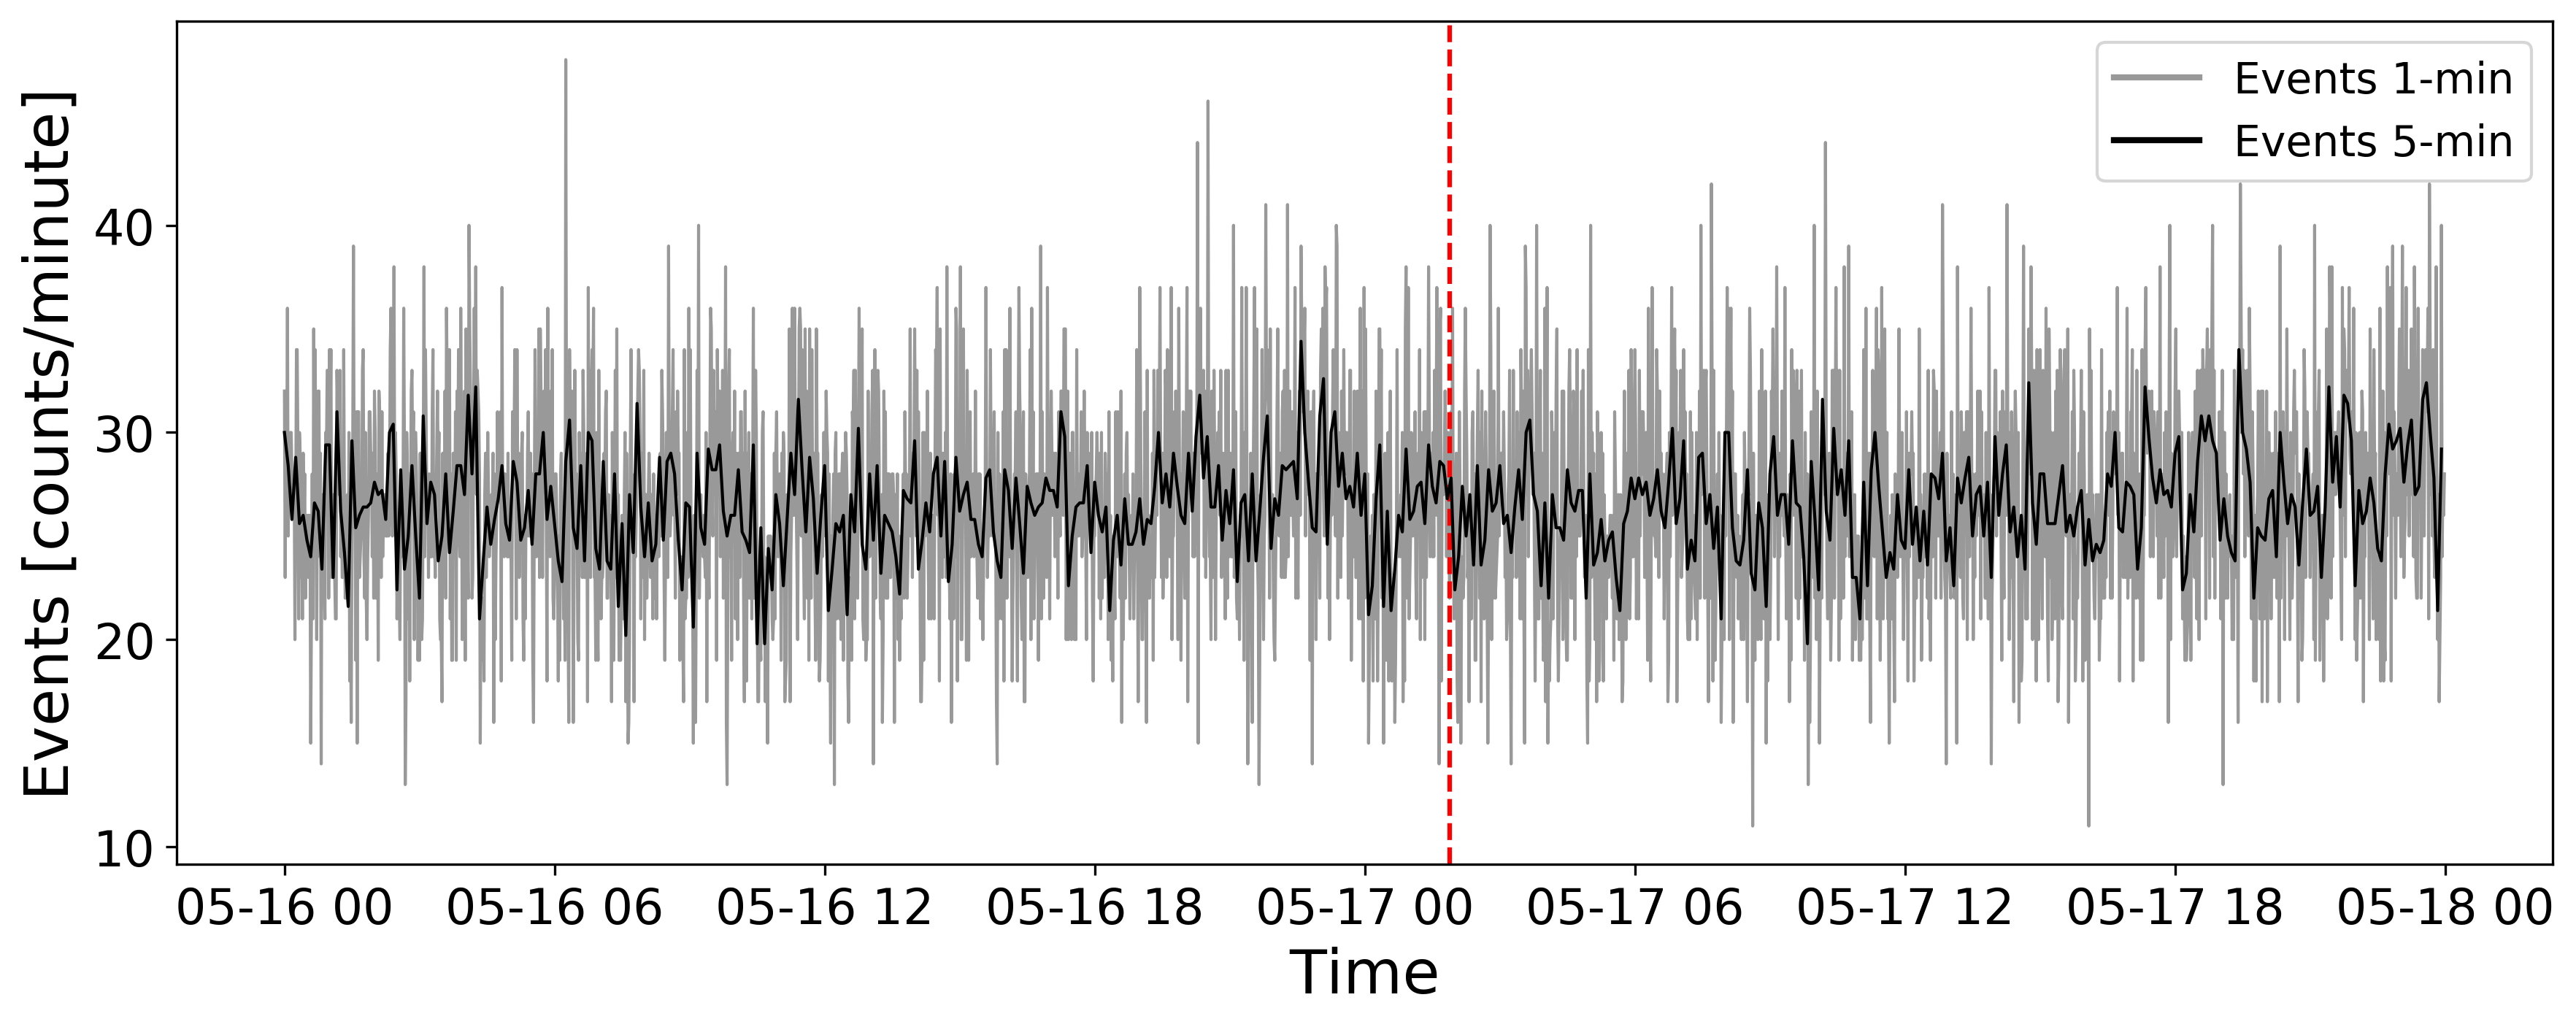
\includegraphics[width=0.48\columnwidth]{GLE71_3001.png}
		\label{fig:GLE71_3001}}
	
	\caption{HiSPARC data for stations 8001 and 3001 around the epoch of GLE 71. The plot shows the minute-averaged and 5-minute-averaged trigger events between detectors within the station. The vertical red, dashed line depicts the approximate onset time of the GLE.}
	\label{fig:GLE_71}
\end{figure}


Figure~\ref{fig:GLE_72}...

\begin{figure}[ht]
	\centering
	\subfloat[HS 501 (Nikhef)]{
		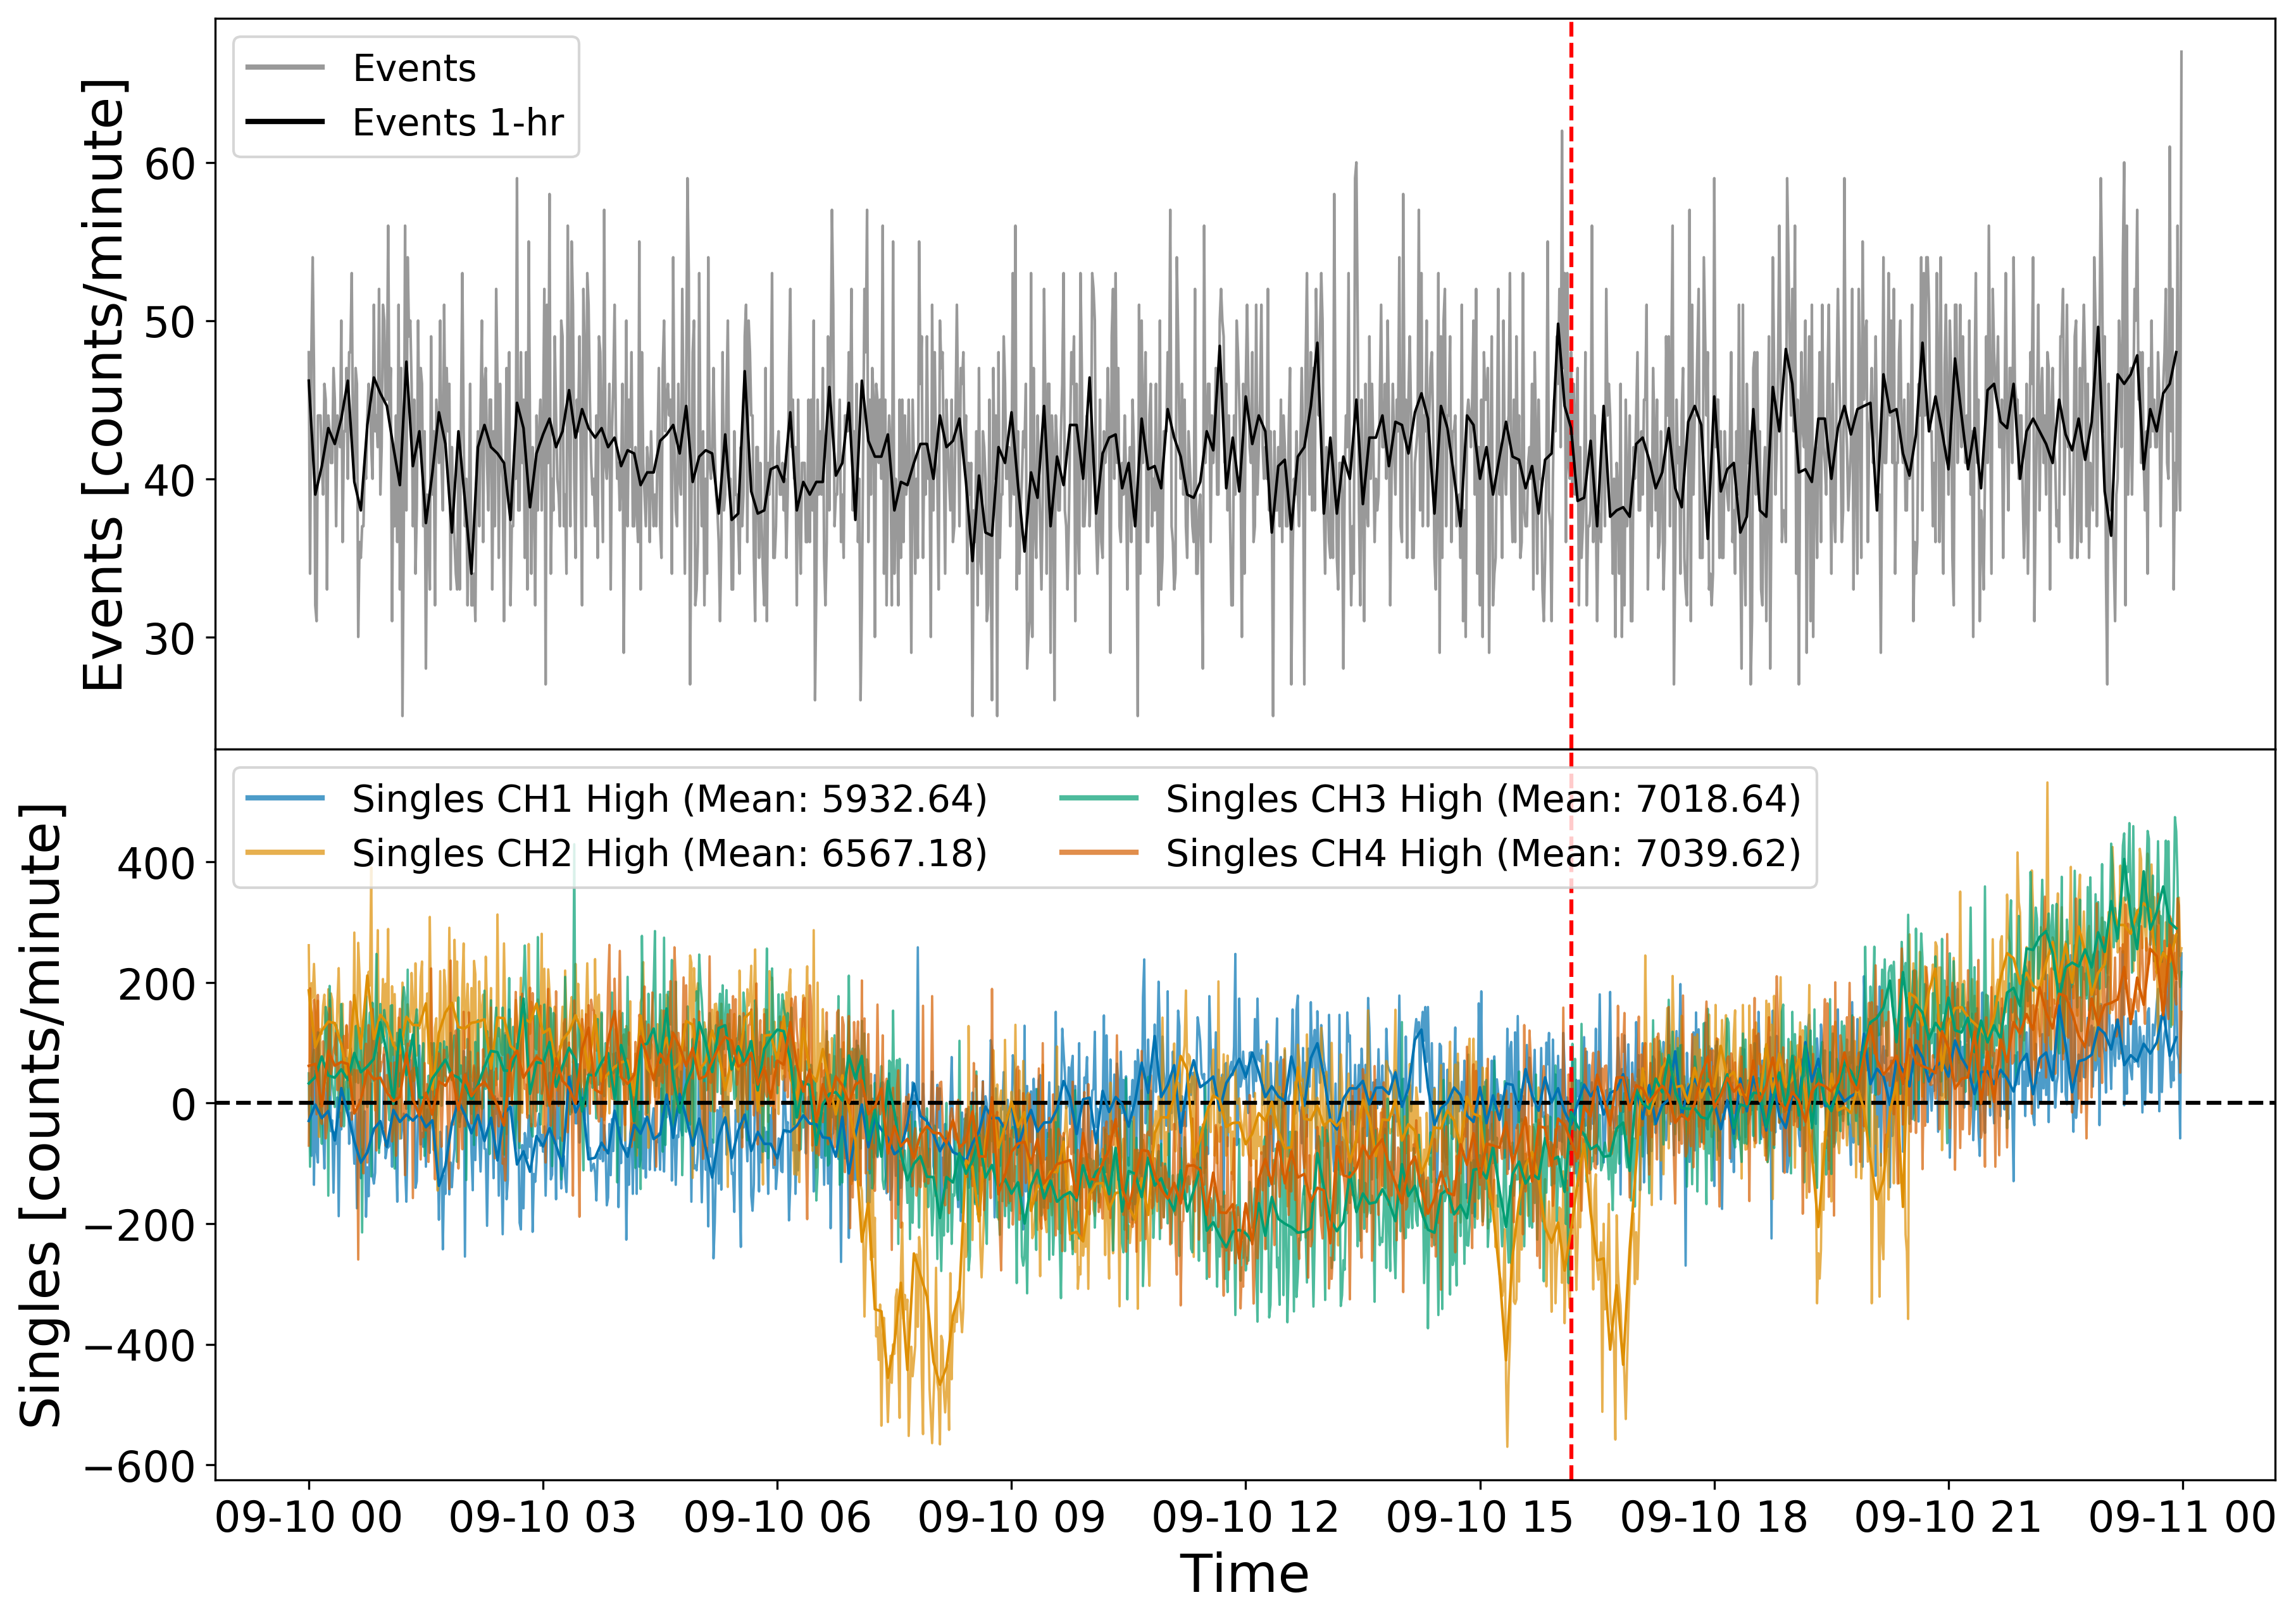
\includegraphics[width=0.48\columnwidth]{GLE72_501.png}
		\label{fig:GLE72_501}}
	%\qquad
	\subfloat[HS 203 (College Hageveld)]{
		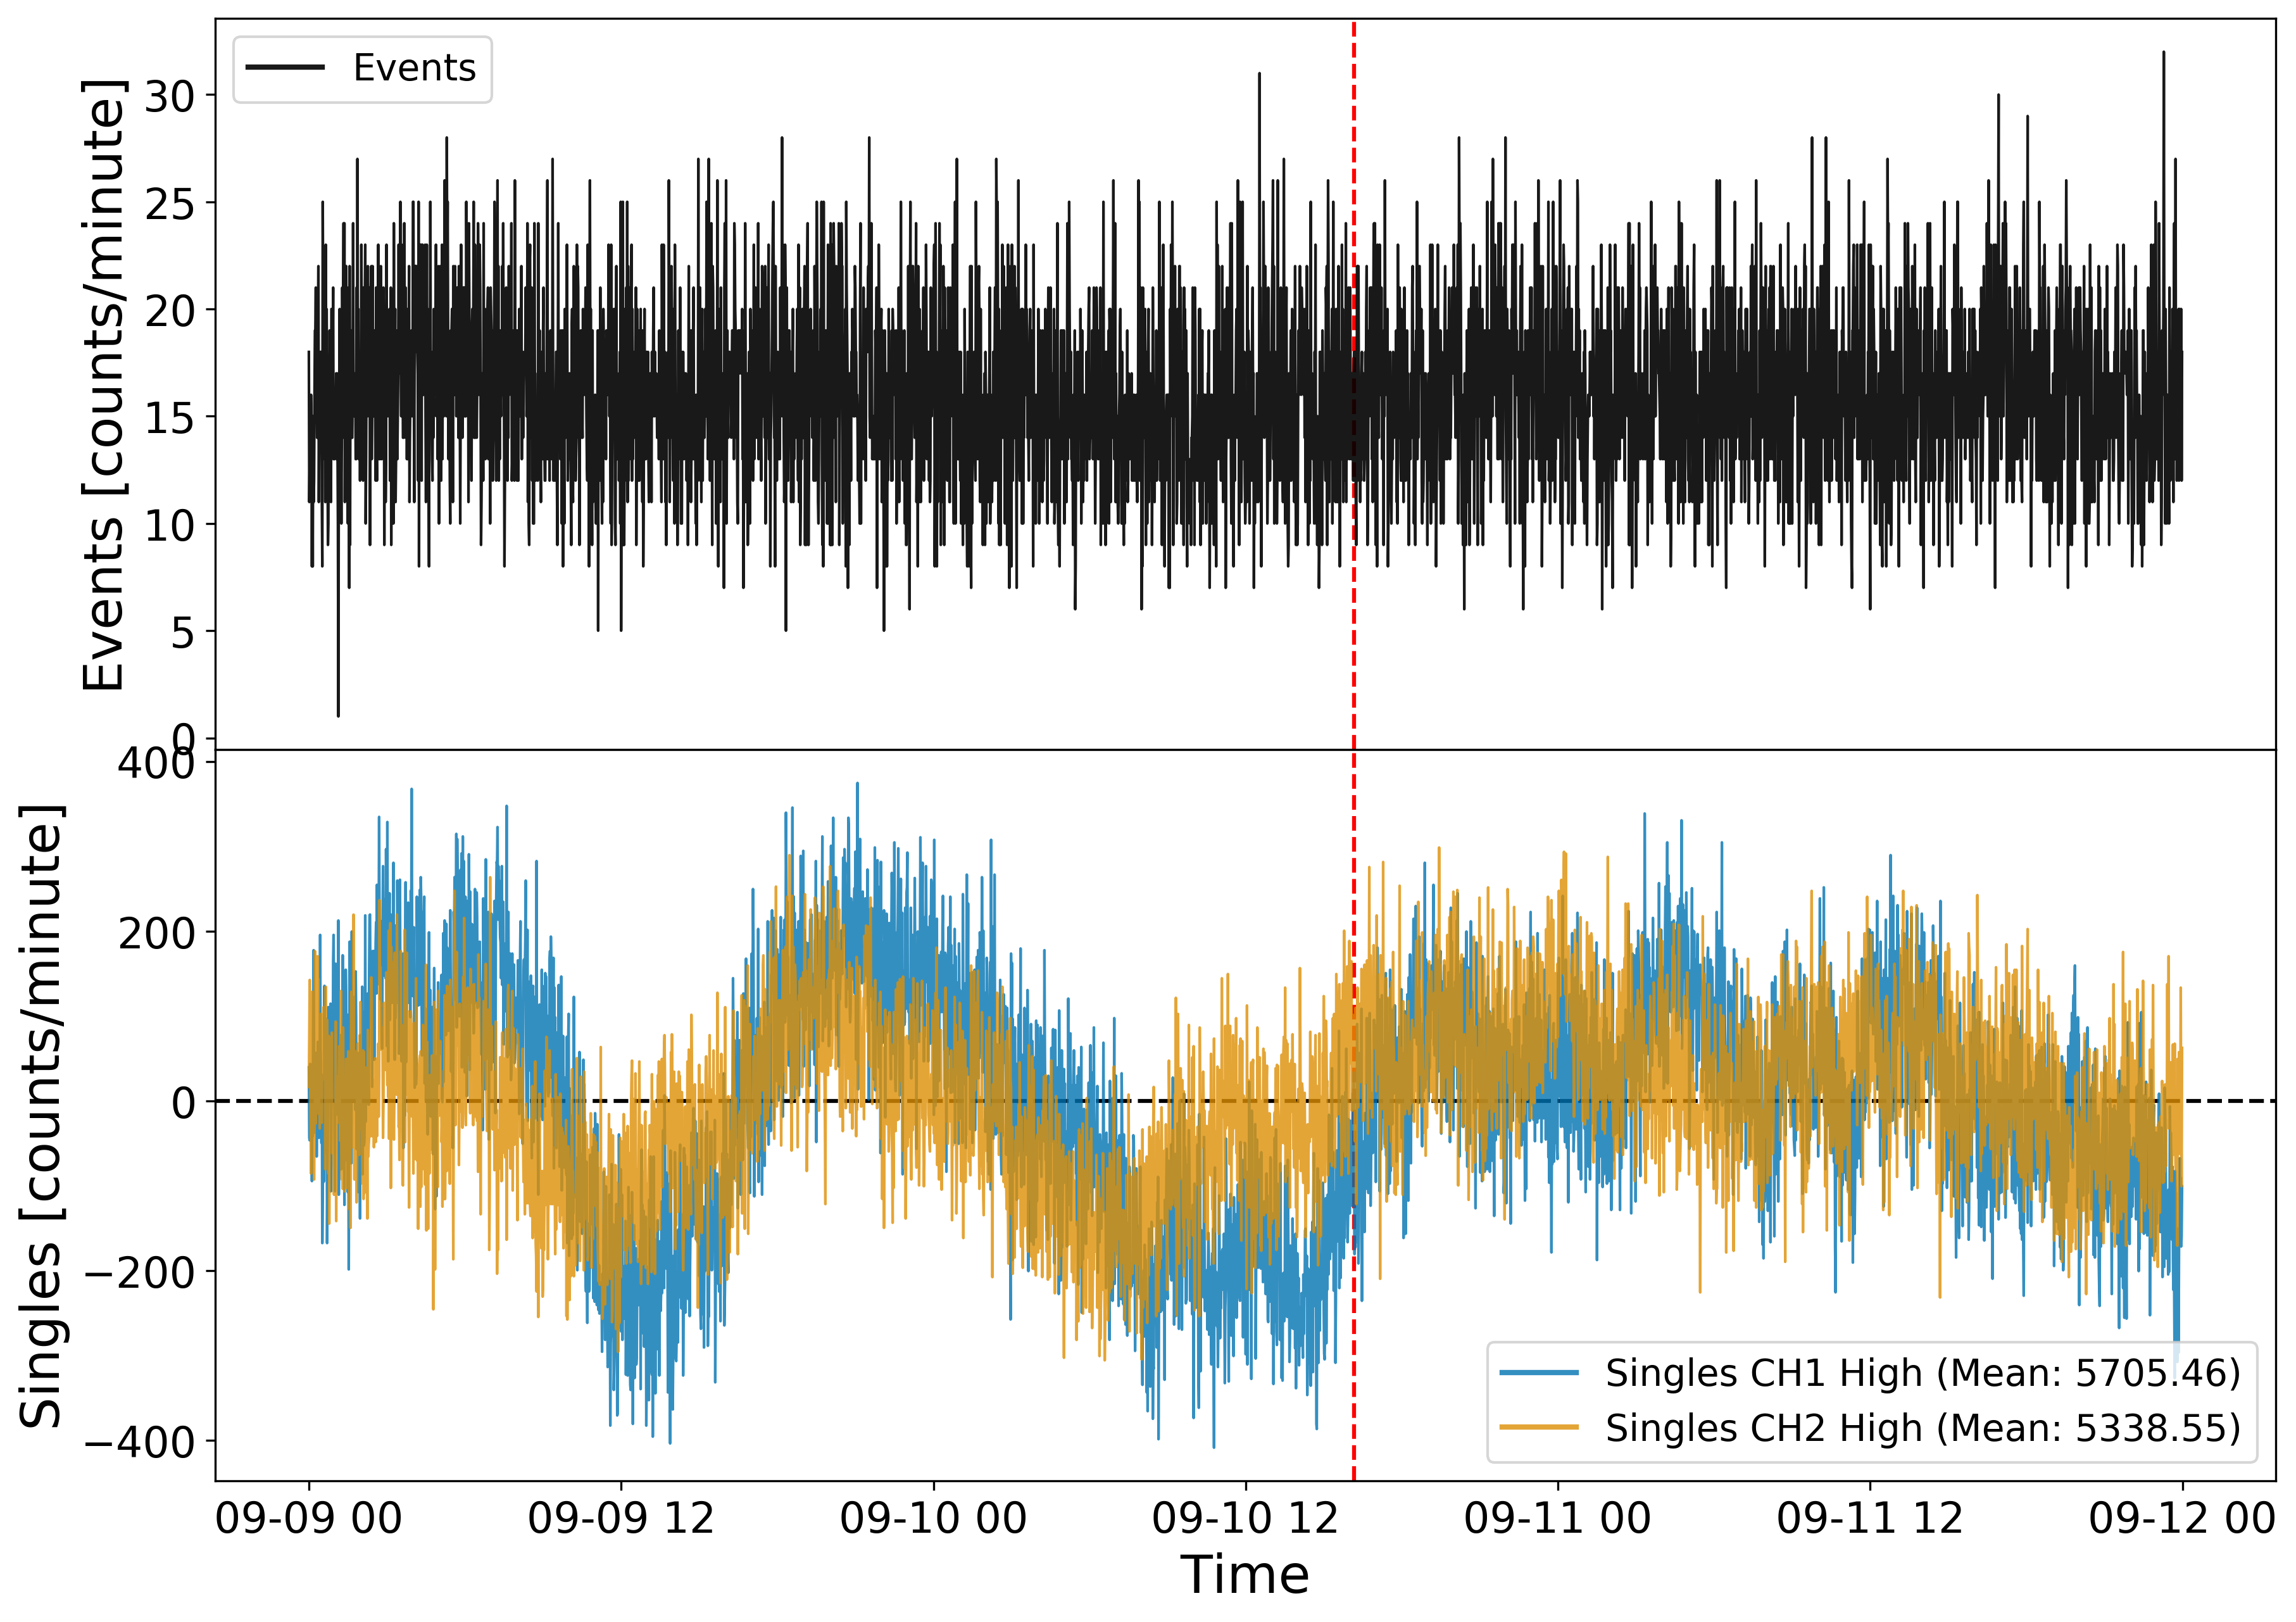
\includegraphics[width=0.48\columnwidth]{GLE72_203.png}
		\label{fig:GLE72_203}} \\
	
	\qquad
	
	\subfloat[HS 8001 (Eindhoven)]{
		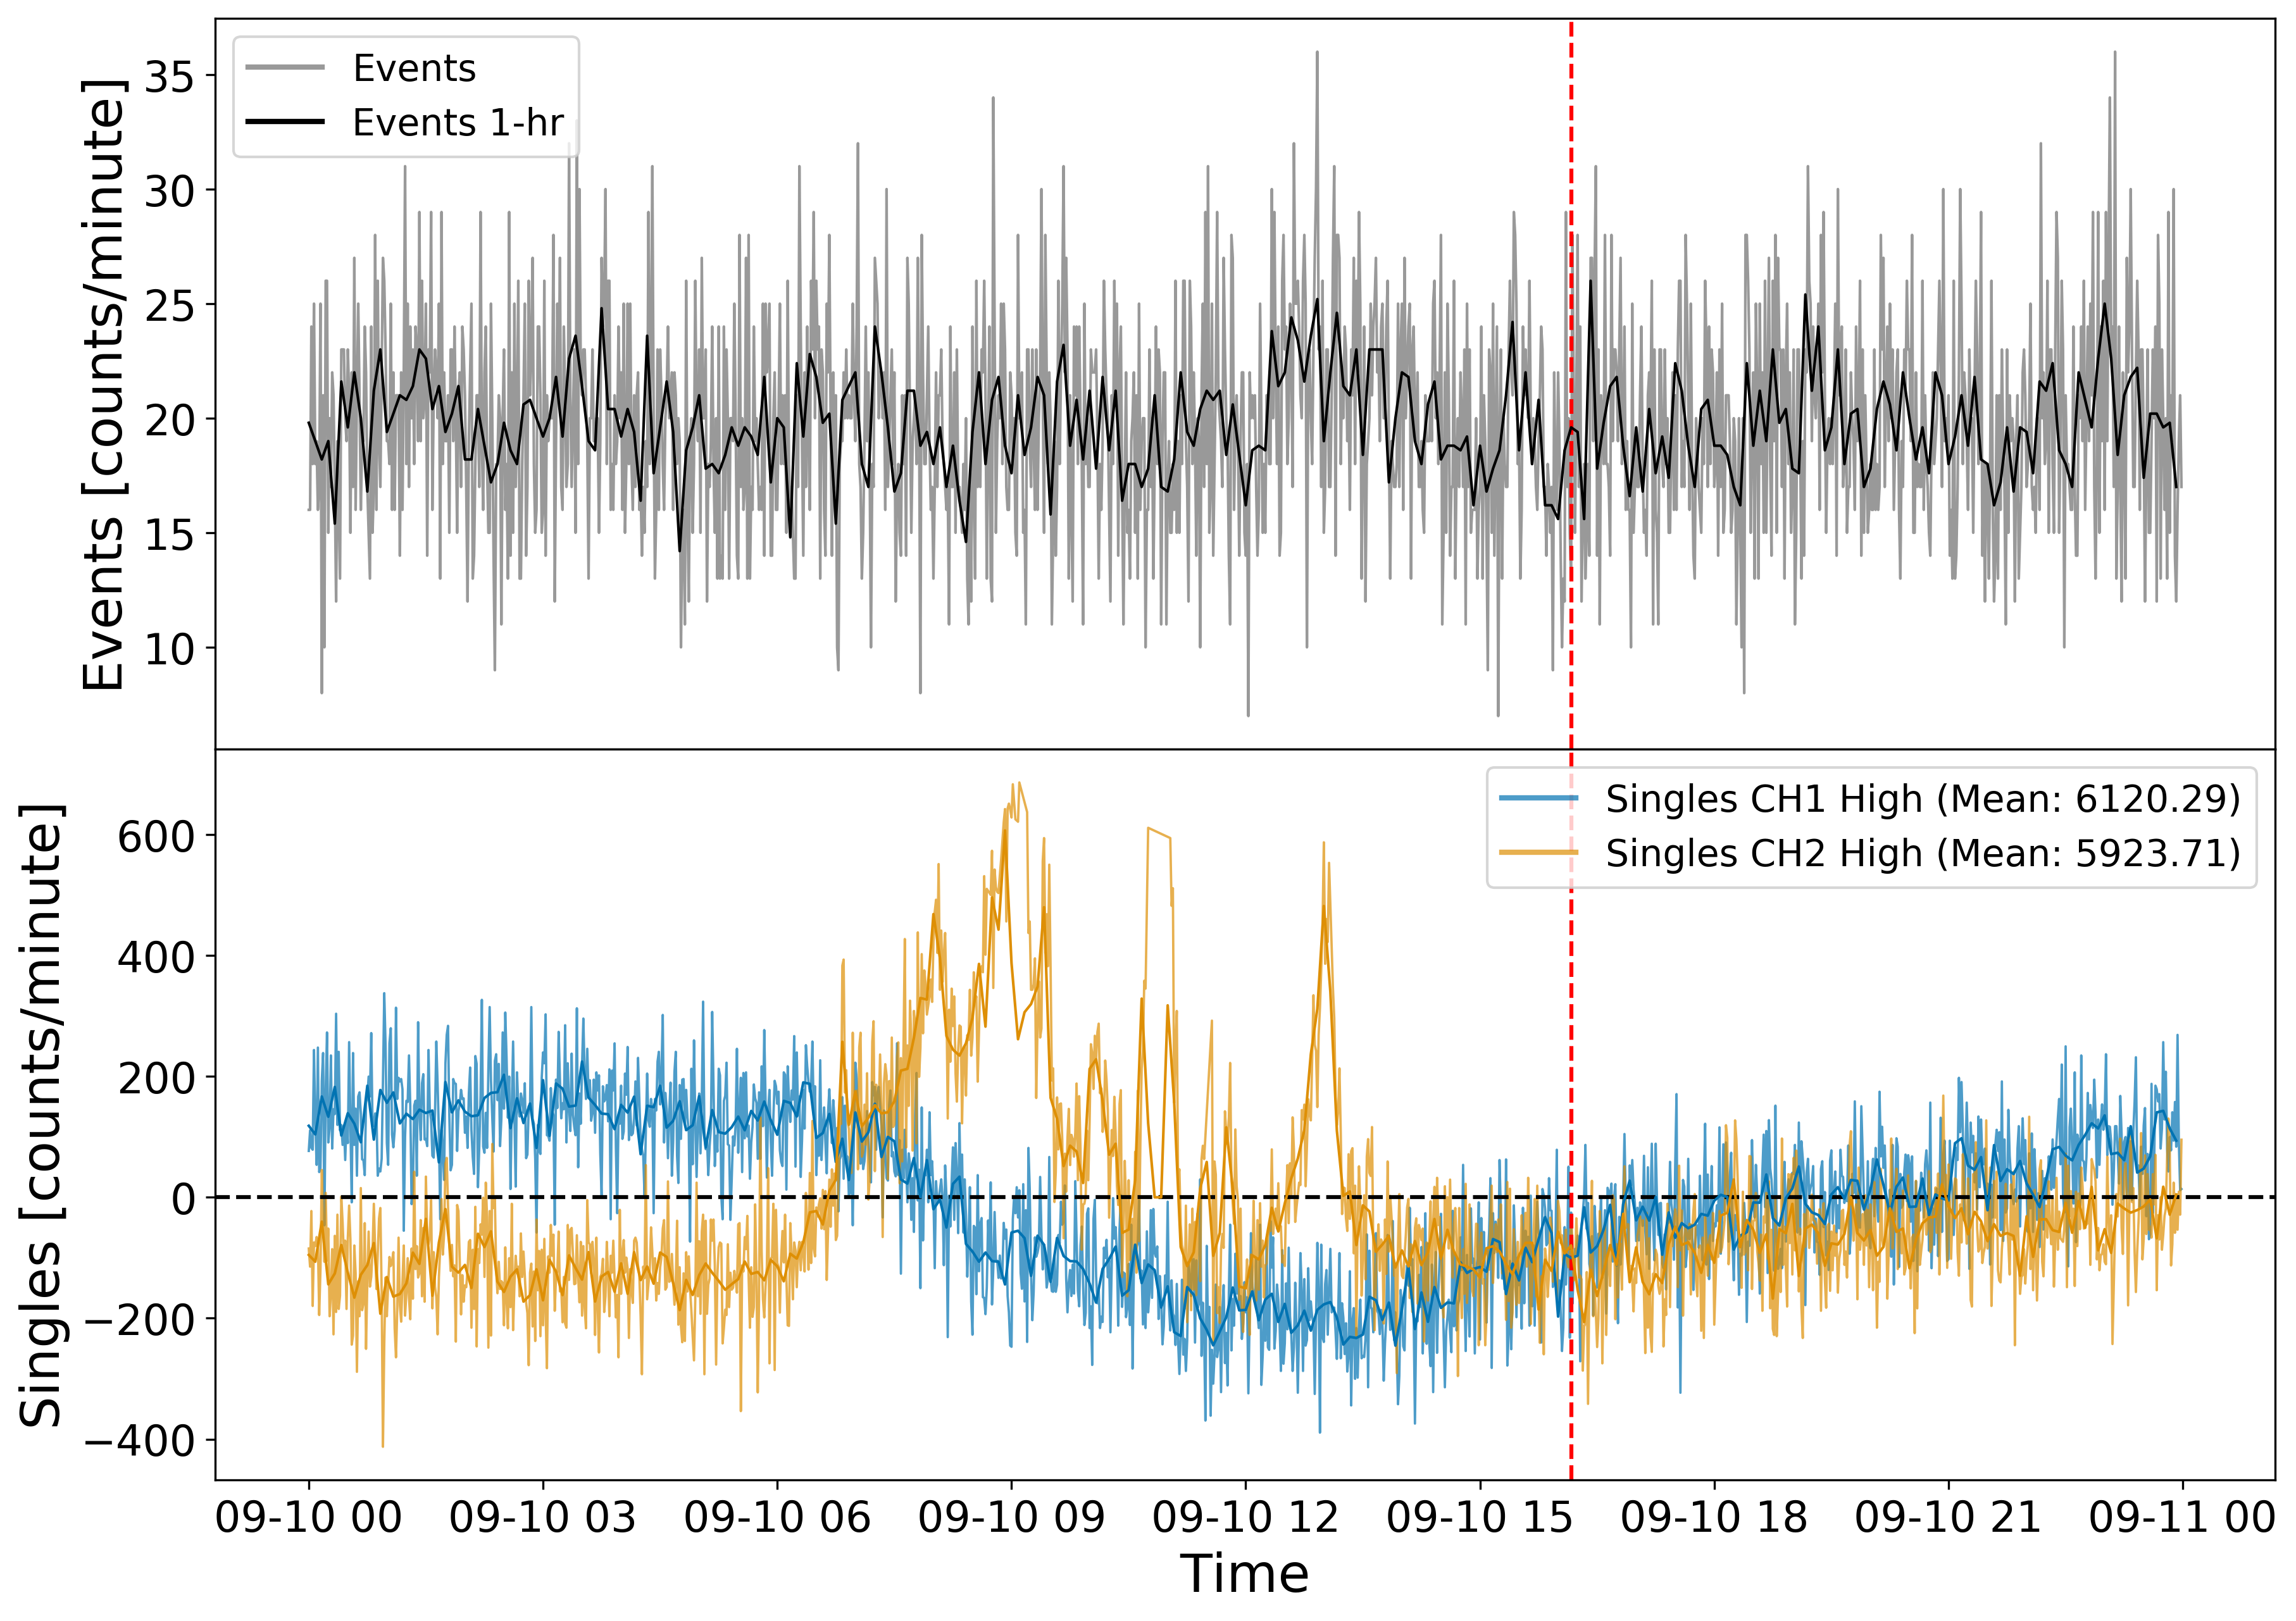
\includegraphics[width=0.48\columnwidth]{GLE72_8001.png}
		\label{fig:GLE72_8001}}
	%\qquad
	\subfloat[HS 14001 (Birmingham University)]{
		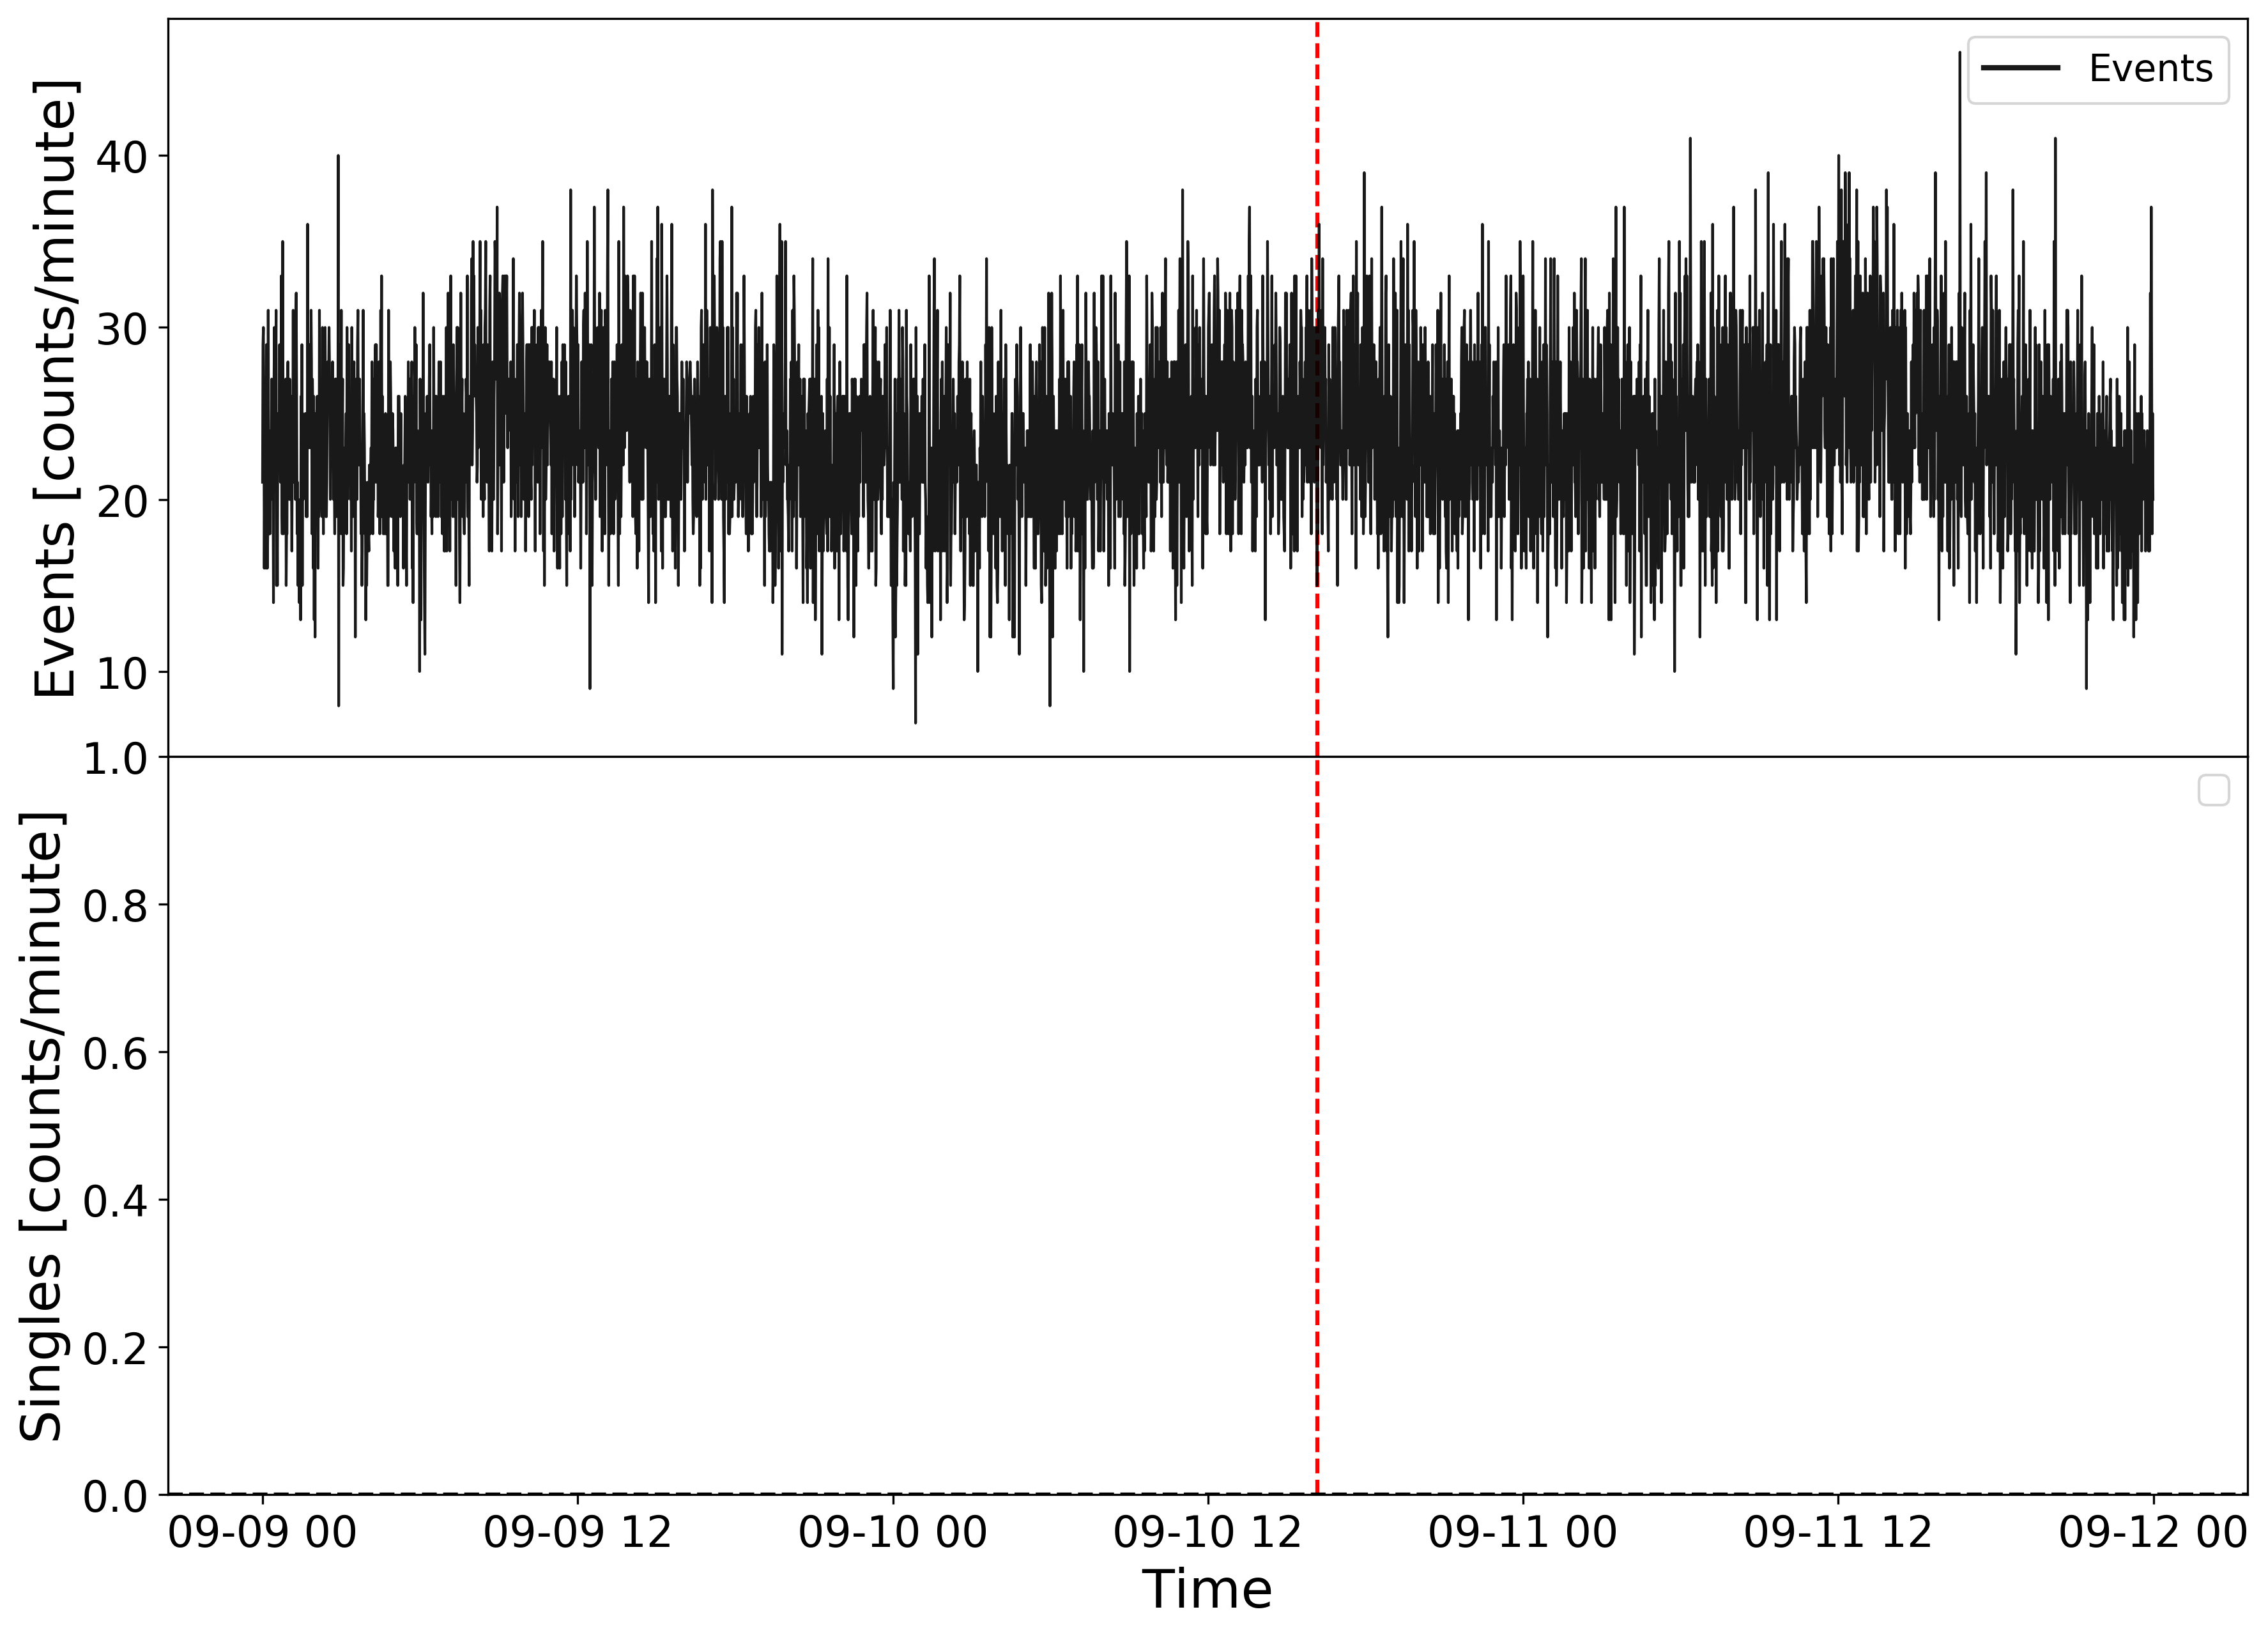
\includegraphics[width=0.48\columnwidth]{GLE72_14001.png}
		\label{fig:GLE72_14001}}
	
	\caption{HiSPARC data for 4 stations around the epoch of GLE 72. The top panel of each subplot shows the minute-averaged trigger events between detectors within the station, while the bottom panel shows the mean-shifted, minute-averaged counts by each individual detector in the station. The vertical red, dashed line depicts the approximate onset time of the GLE.}
	\label{fig:GLE_72}
\end{figure}

... no clear GLE seen...

%%%%%%%%%%%%%%%%%%%%%%%%%%%%%%%%%%%%%%%%%%%%%%%%%%%%%%%%%%%%%%%%%%%%%
\subsection{HiSPARC Observations of Forbush Decreases}

Figure~\ref{fig:FD_201203}...

\begin{figure}[ht]
	\centering
	\subfloat[HS 501 (Nikhef)]{
		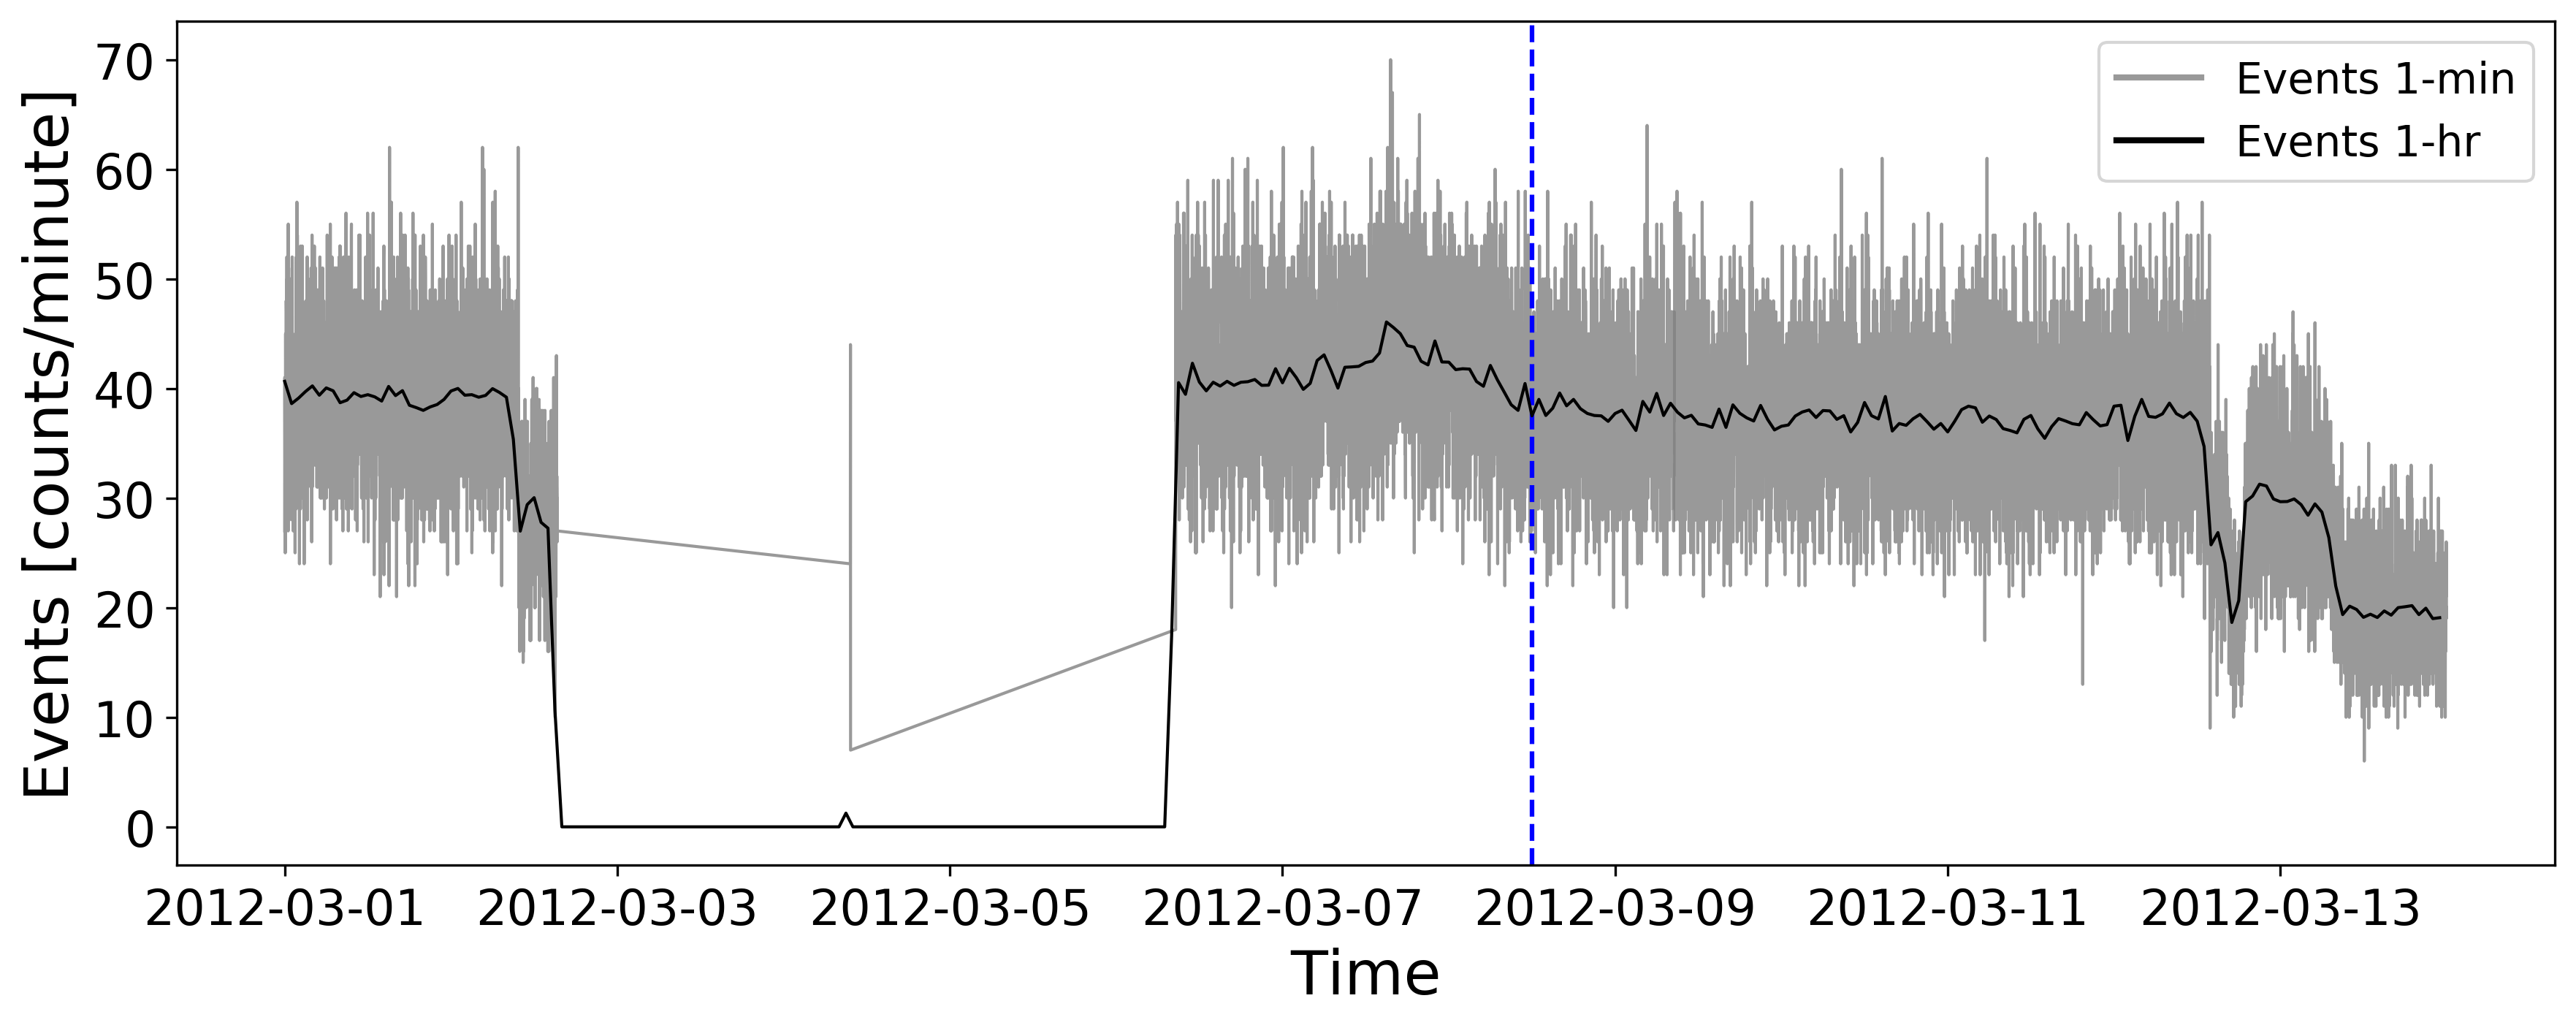
\includegraphics[width=0.48\columnwidth]{FD_201203_501.png}
		\label{fig:FD_201203_501}}
	%\qquad
	\subfloat[HS 8001 (Eindhoven)]{
		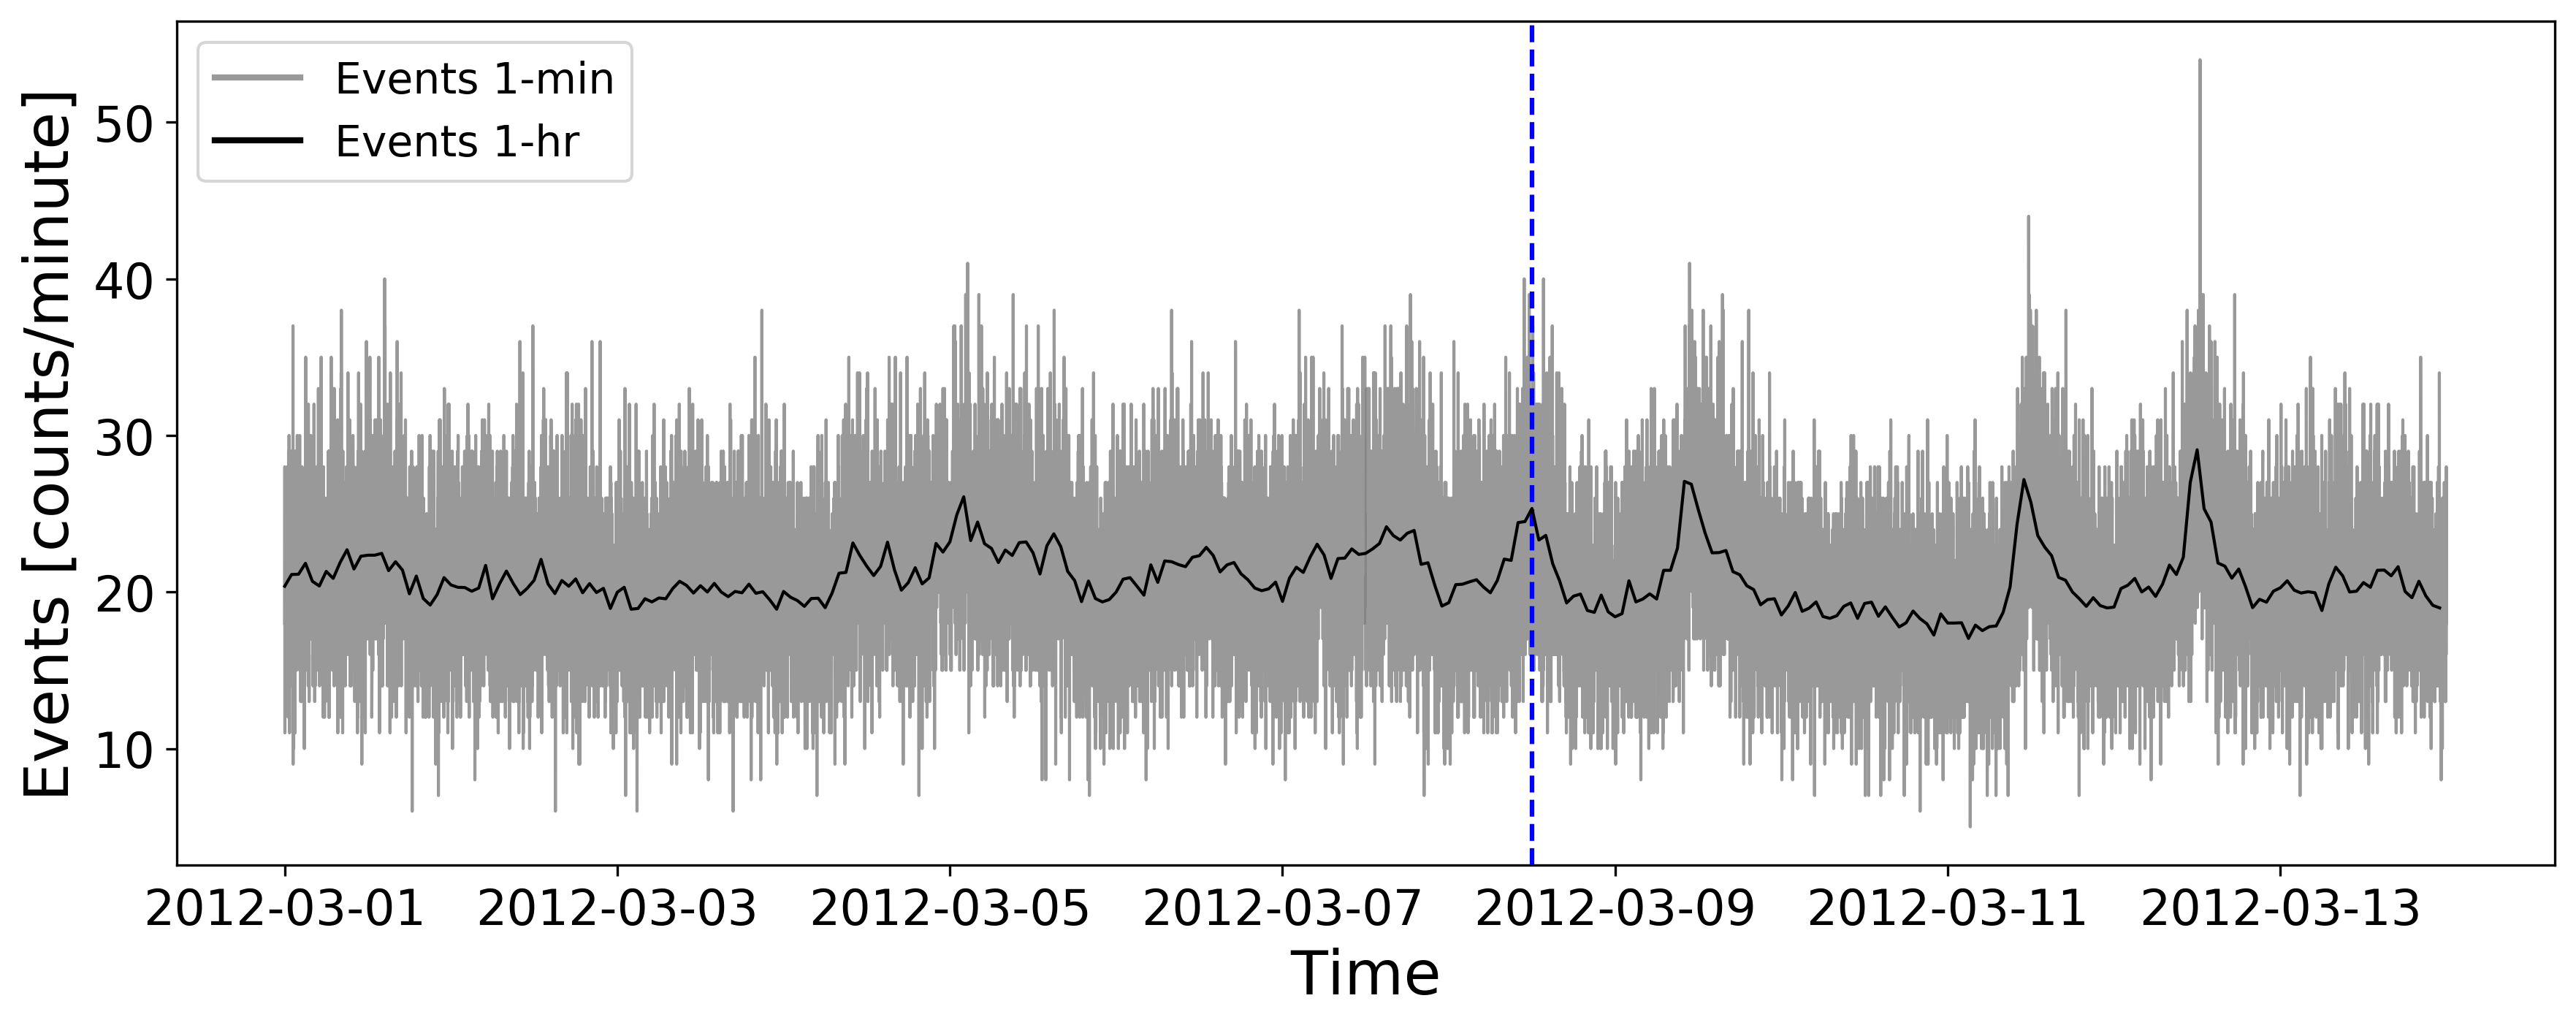
\includegraphics[width=0.48\columnwidth]{FD_201203_8001.png}
		\label{fig:FD_201203_8001}}
	
	\caption{HiSPARC data for stations 501 and 8001 around the epoch of the FD in March 2012. The plot shows the minute-averaged and hourly-averaged trigger events between detectors within the station. The vertical blue-dashed line shows the approximate onset-time of the FD.}
	\label{fig:FD_201203}
\end{figure}


Figure~\ref{fig:FD_201207}...

\begin{figure}[ht]
	\centering
	\subfloat[HS 501 (Nikhef)]{
		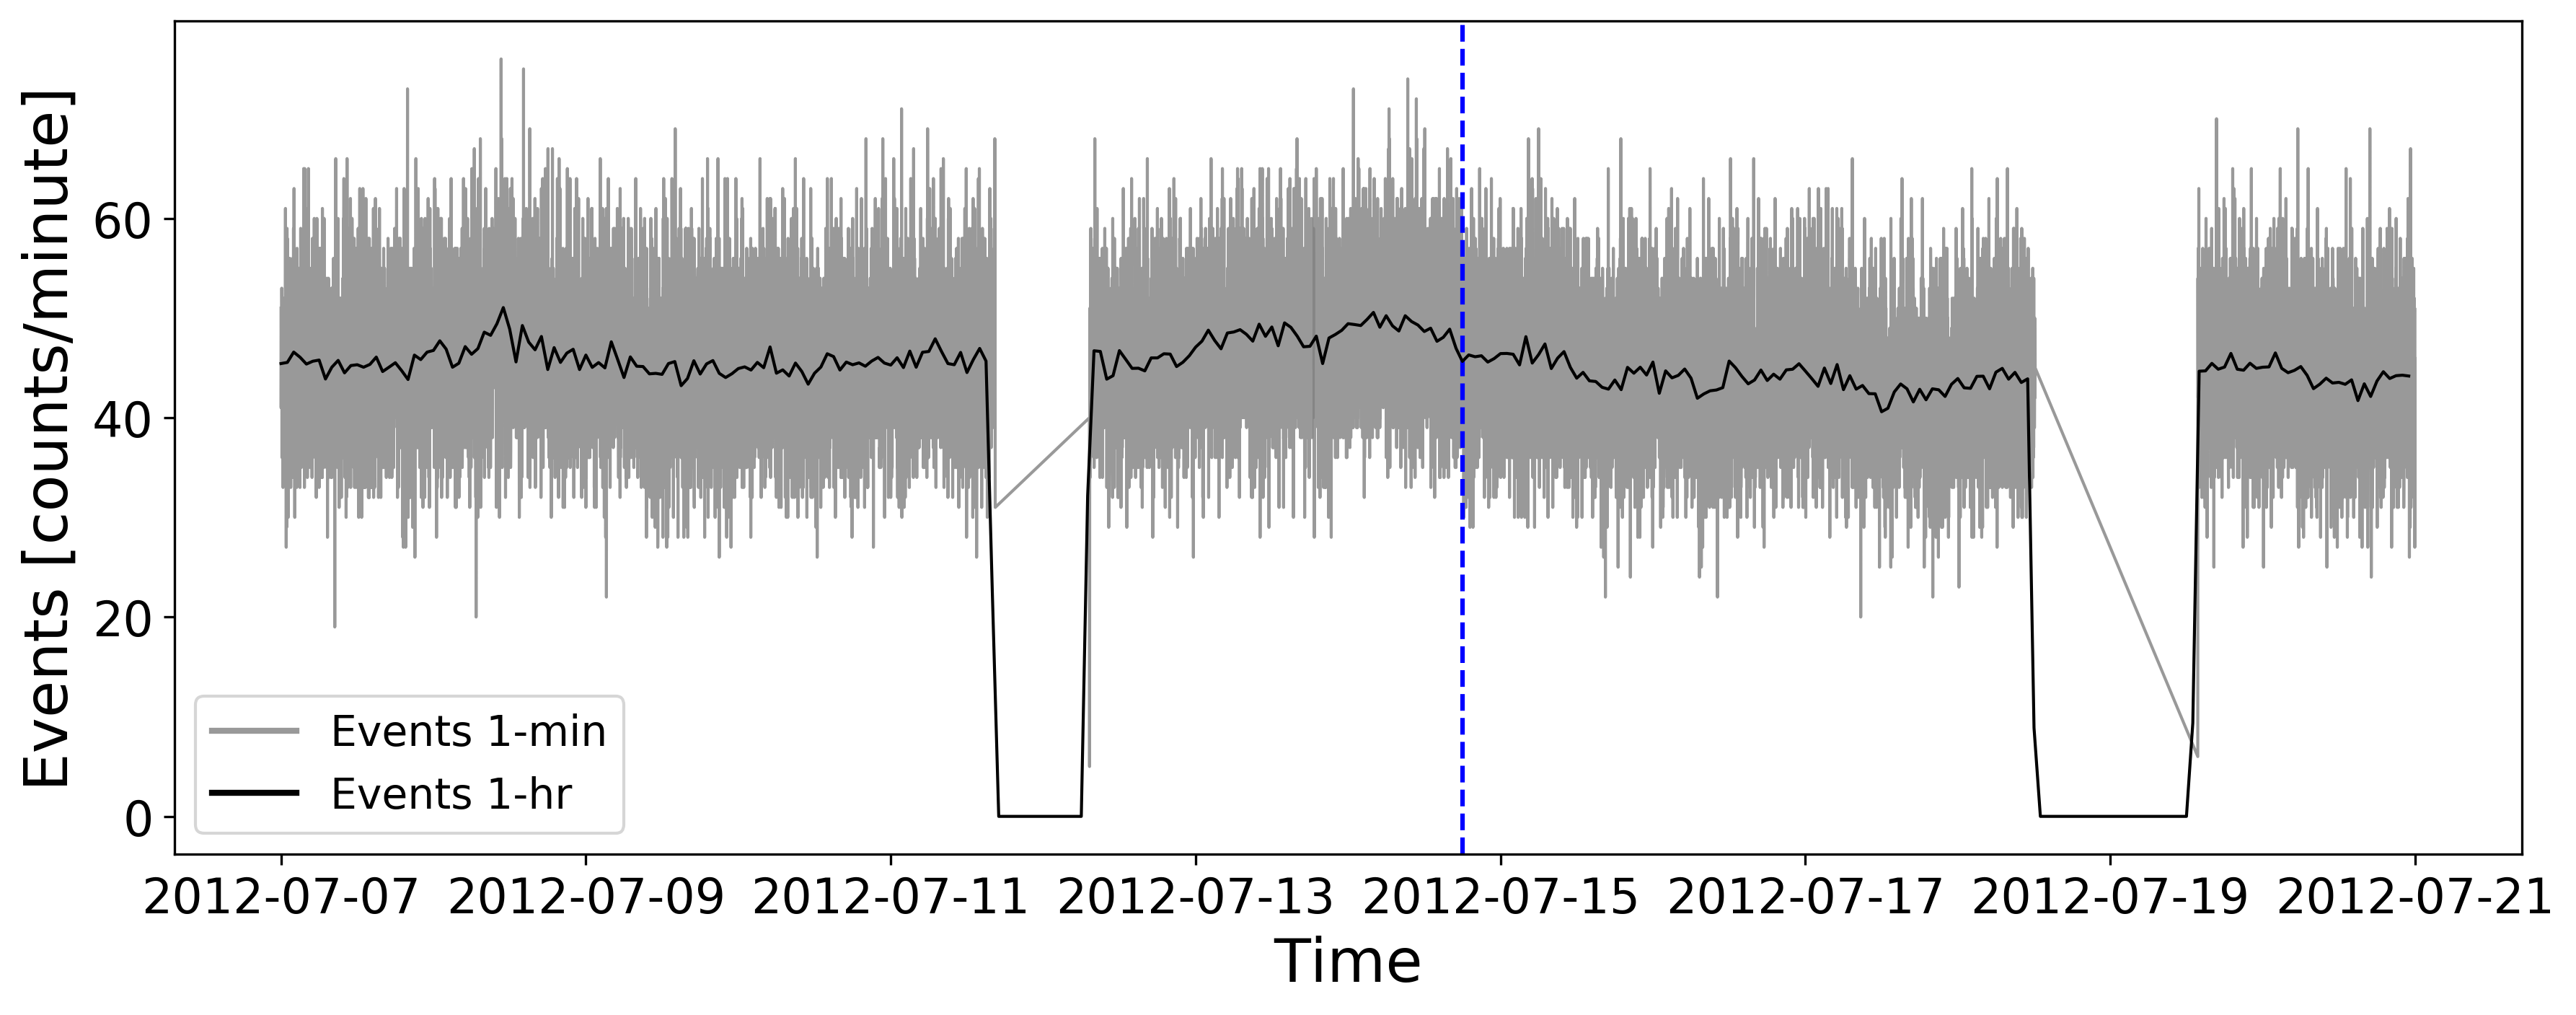
\includegraphics[width=0.48\columnwidth]{FD_201207_501.png}
		\label{fig:FD_201207_501}}
	%\qquad
	\subfloat[HS 8001 (Eindhoven)]{
		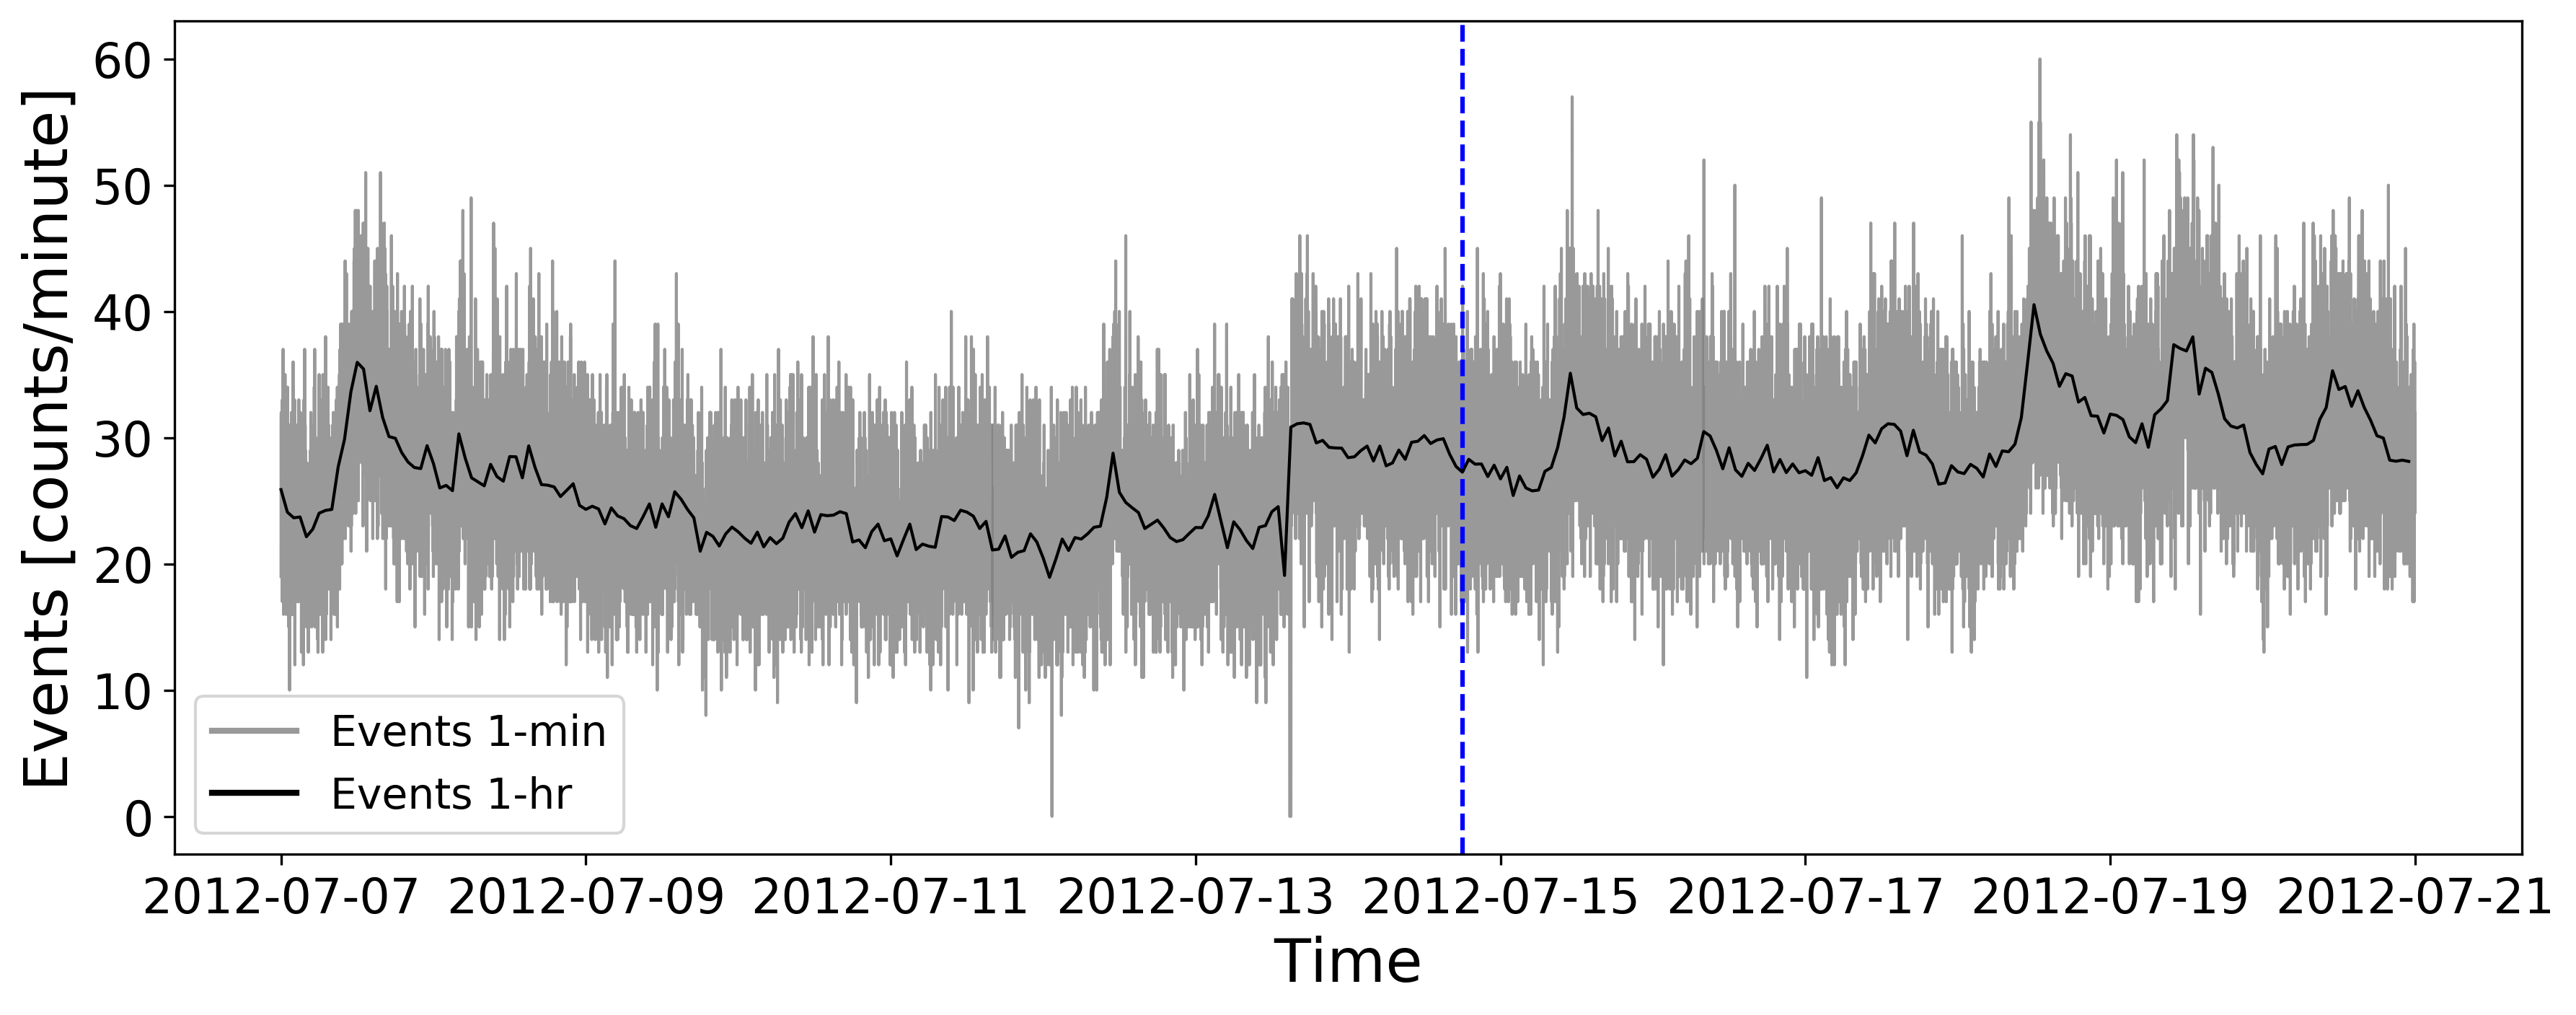
\includegraphics[width=0.48\columnwidth]{FD_201207_8001.png}
		\label{fig:FD_201207_8001}}
	
	\caption{HiSPARC data for stations 501 and 8001 around the epoch of the FD in July 2012. The plot shows the minute-averaged and hourly-averaged trigger events between detectors within the station. The vertical blue-dashed line shows the approximate onset-time of the FD.}
	\label{fig:FD_201207}
\end{figure}



Figure~\ref{fig:FD_201412}...

\begin{figure}[ht]
	\centering
	\subfloat[HS 501 (Nikhef)]{
		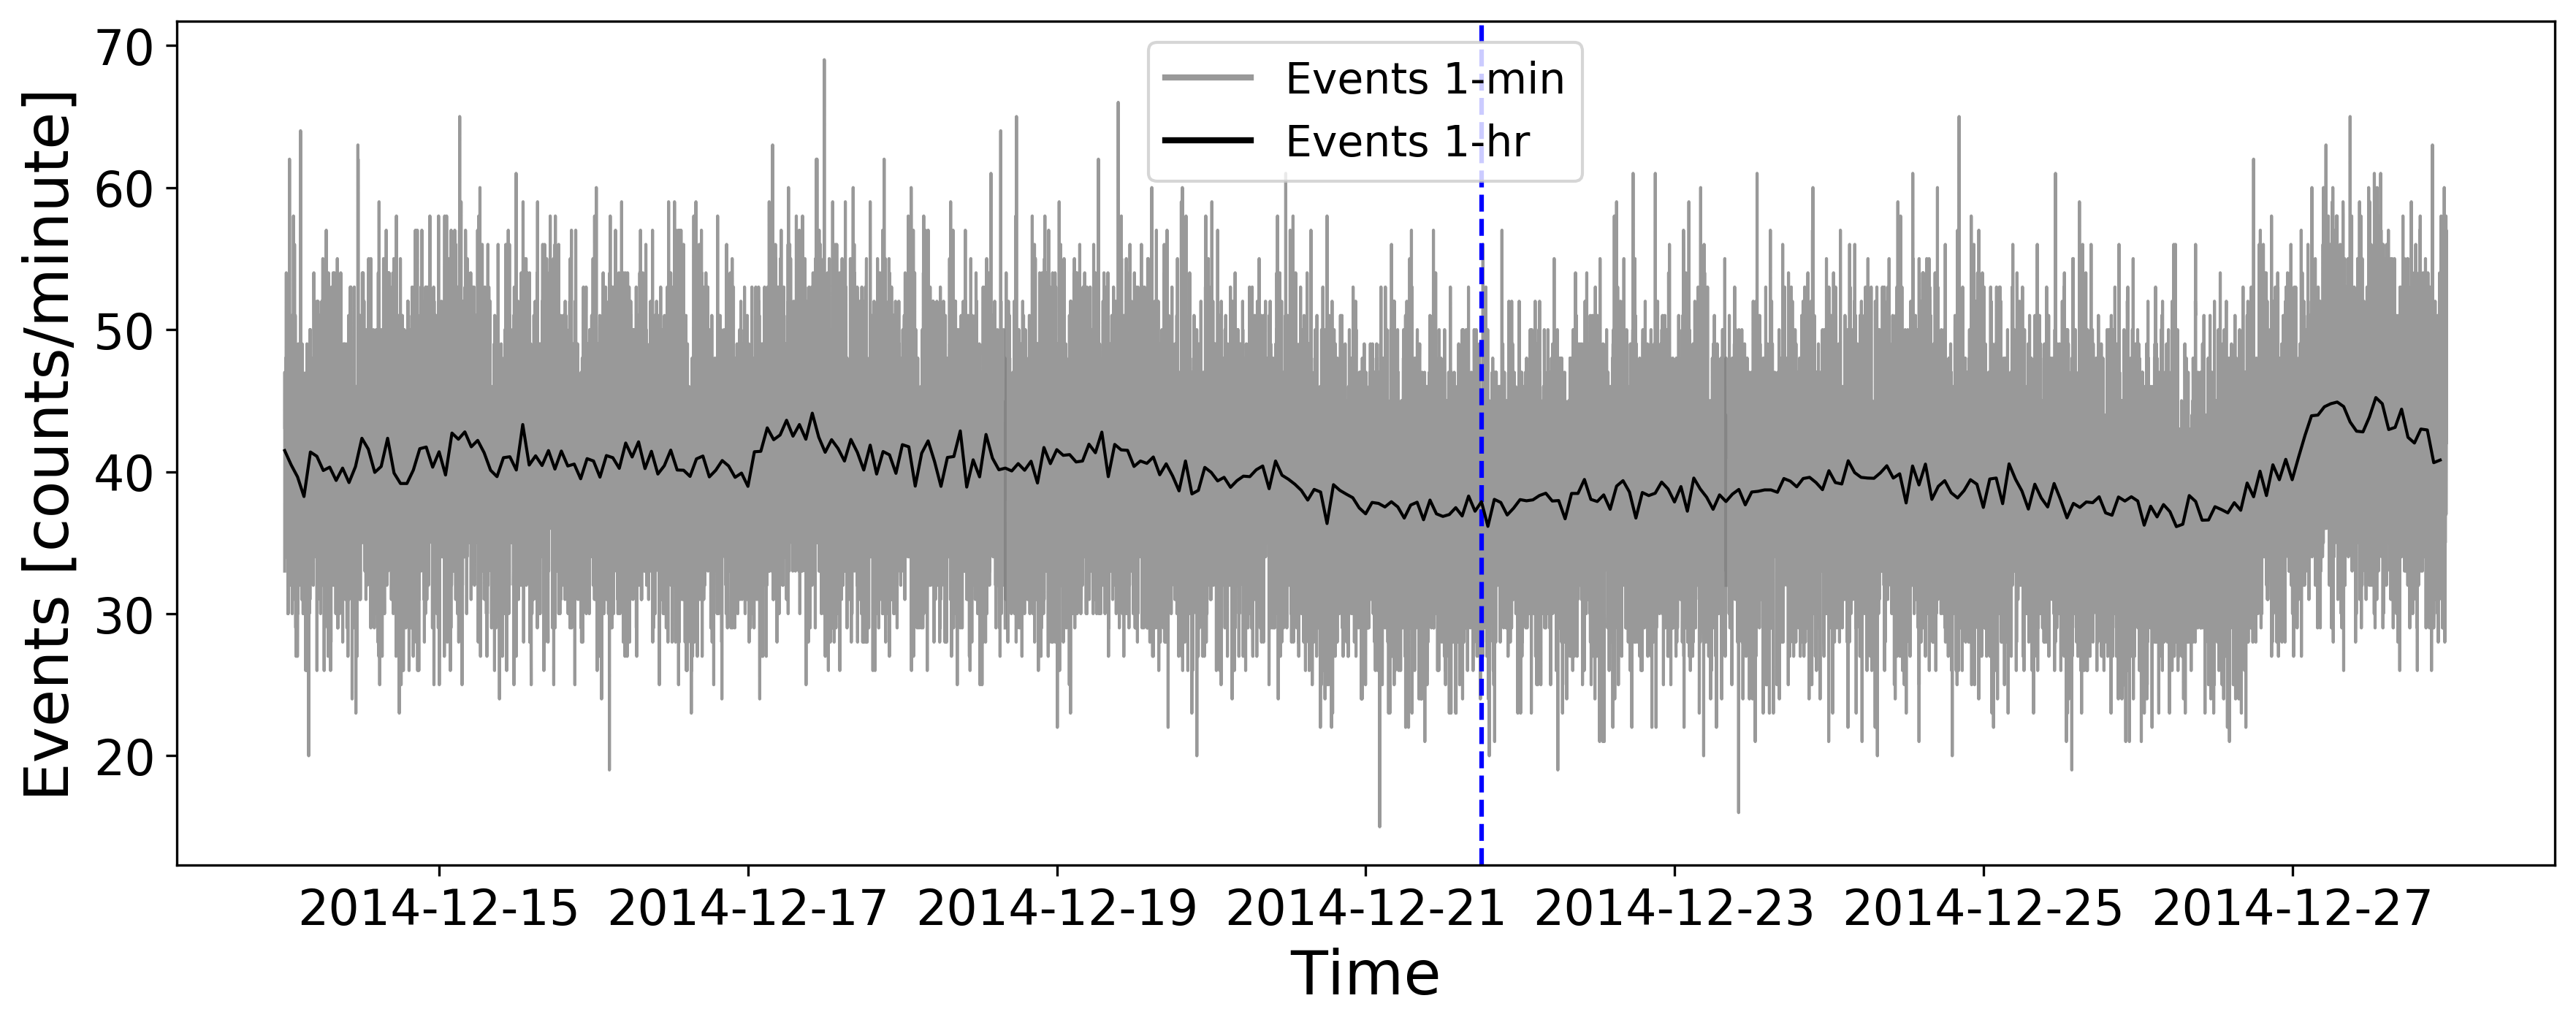
\includegraphics[width=0.48\columnwidth]{FD_201412_501.png}
		\label{fig:FD_201412_501}}
	%\qquad
	\subfloat[HS 203 (College Hageveld)]{
		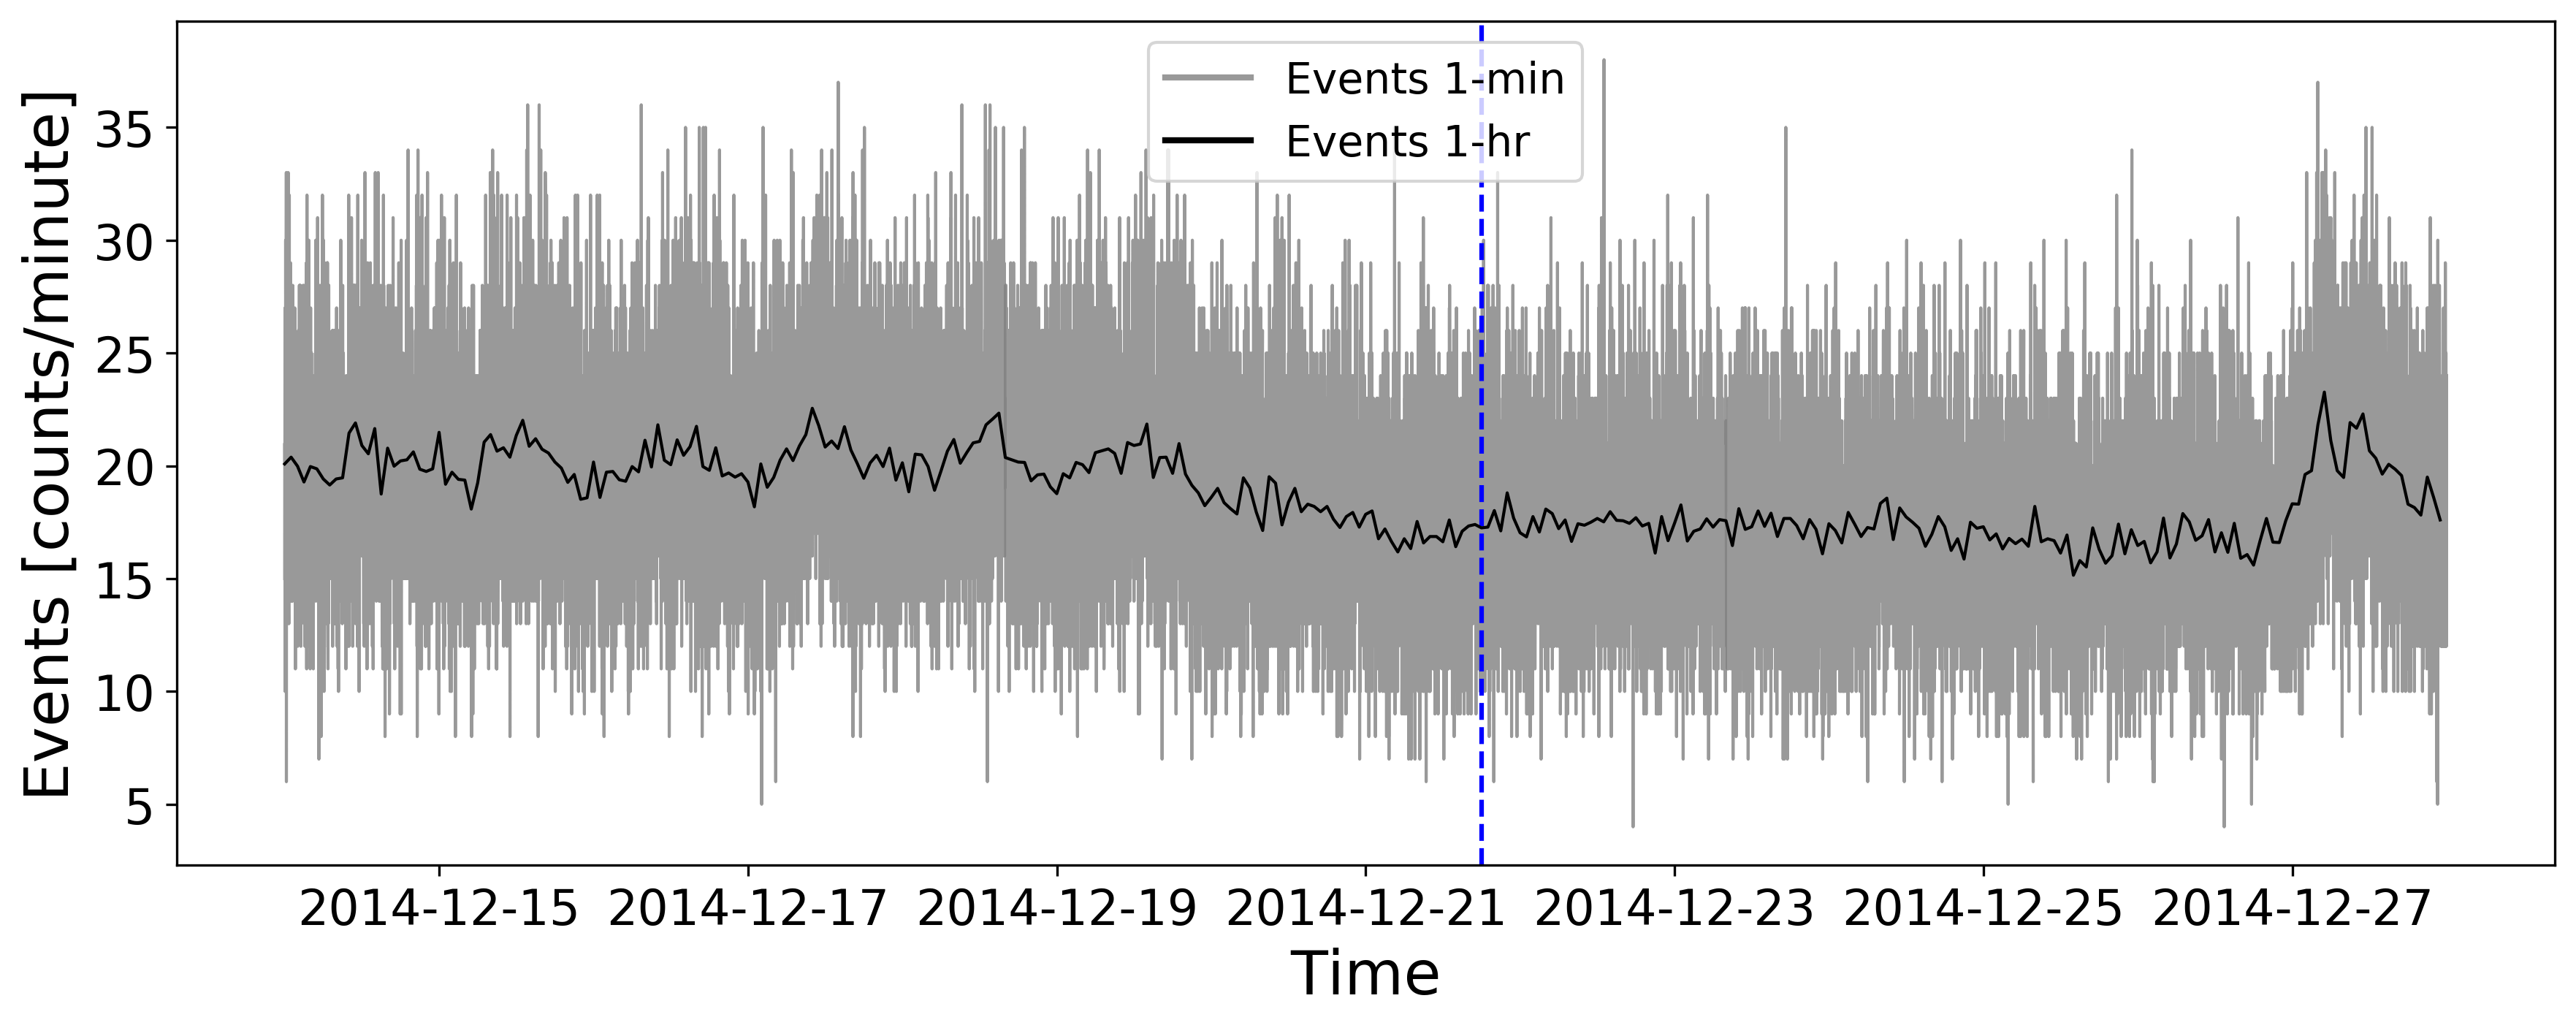
\includegraphics[width=0.48\columnwidth]{FD_201412_203.png}
		\label{fig:FD_201412_203}} \\
	
	\qquad
	
	\subfloat[HS 3001 (Leiden)]{
		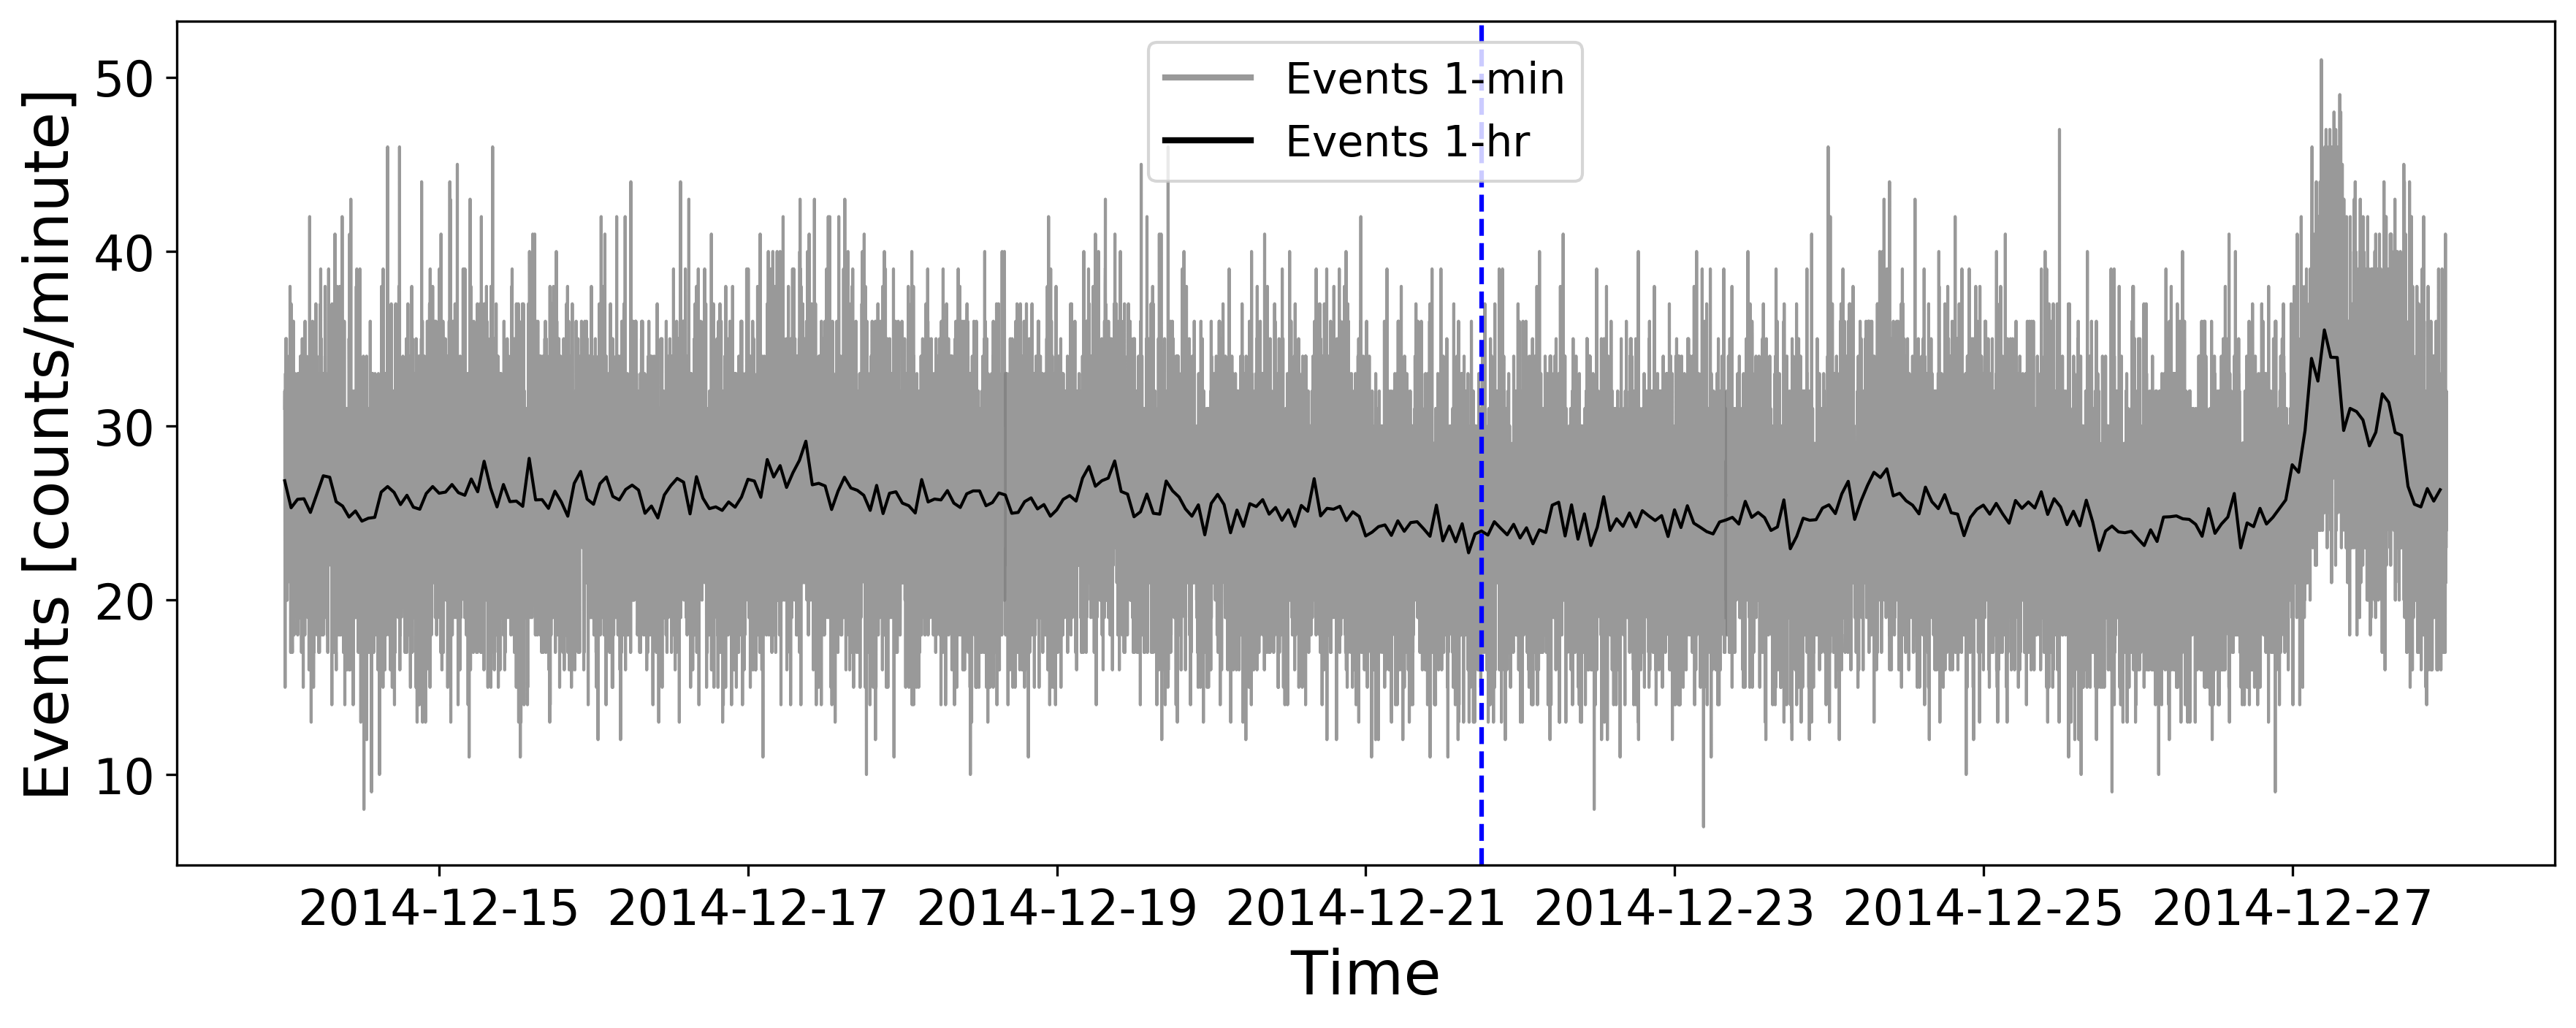
\includegraphics[width=0.48\columnwidth]{FD_201412_3001.png}
		\label{fig:FD_201412_3001}}
	%\qquad
	\subfloat[HS 14001 (Birmingham University)]{
		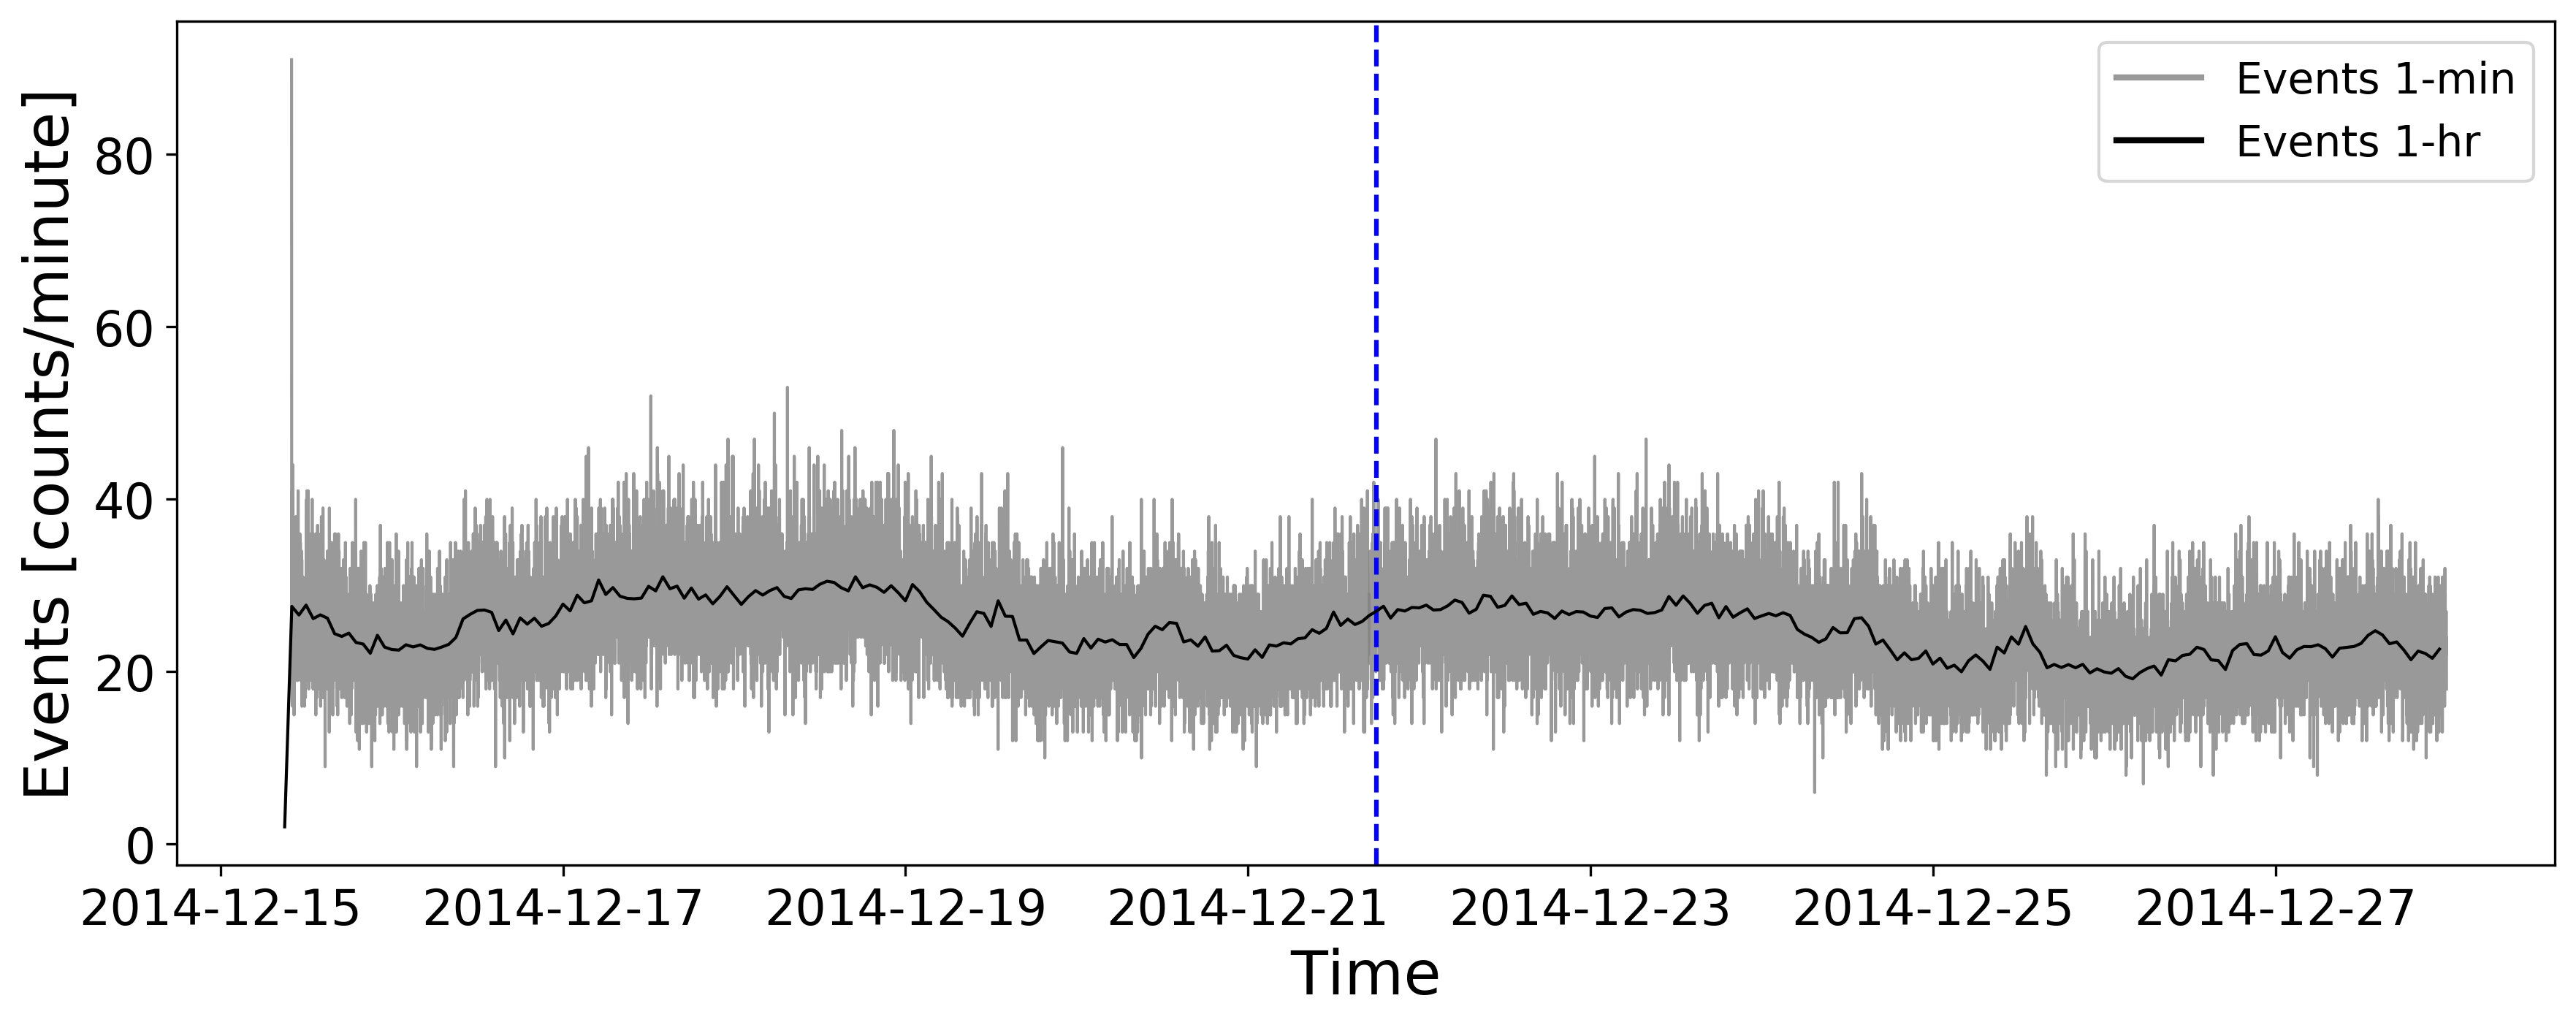
\includegraphics[width=0.48\columnwidth]{FD_201412_14001.png}
		\label{fig:FD_201412_14001}}
	
	\caption{HiSPARC data for 4 stations around the epoch of the FD in December 2014. The plot shows the minute-averaged and hourly-averaged trigger events between detectors within the station. The vertical blue-dashed line shows the approximate onset-time of the FD.}
	\label{fig:FD_201412}
\end{figure}



Figure~\ref{fig:FD_GLE72}...

\begin{figure}[ht]
	\centering
	\subfloat[HS 501 (Nikhef)]{
		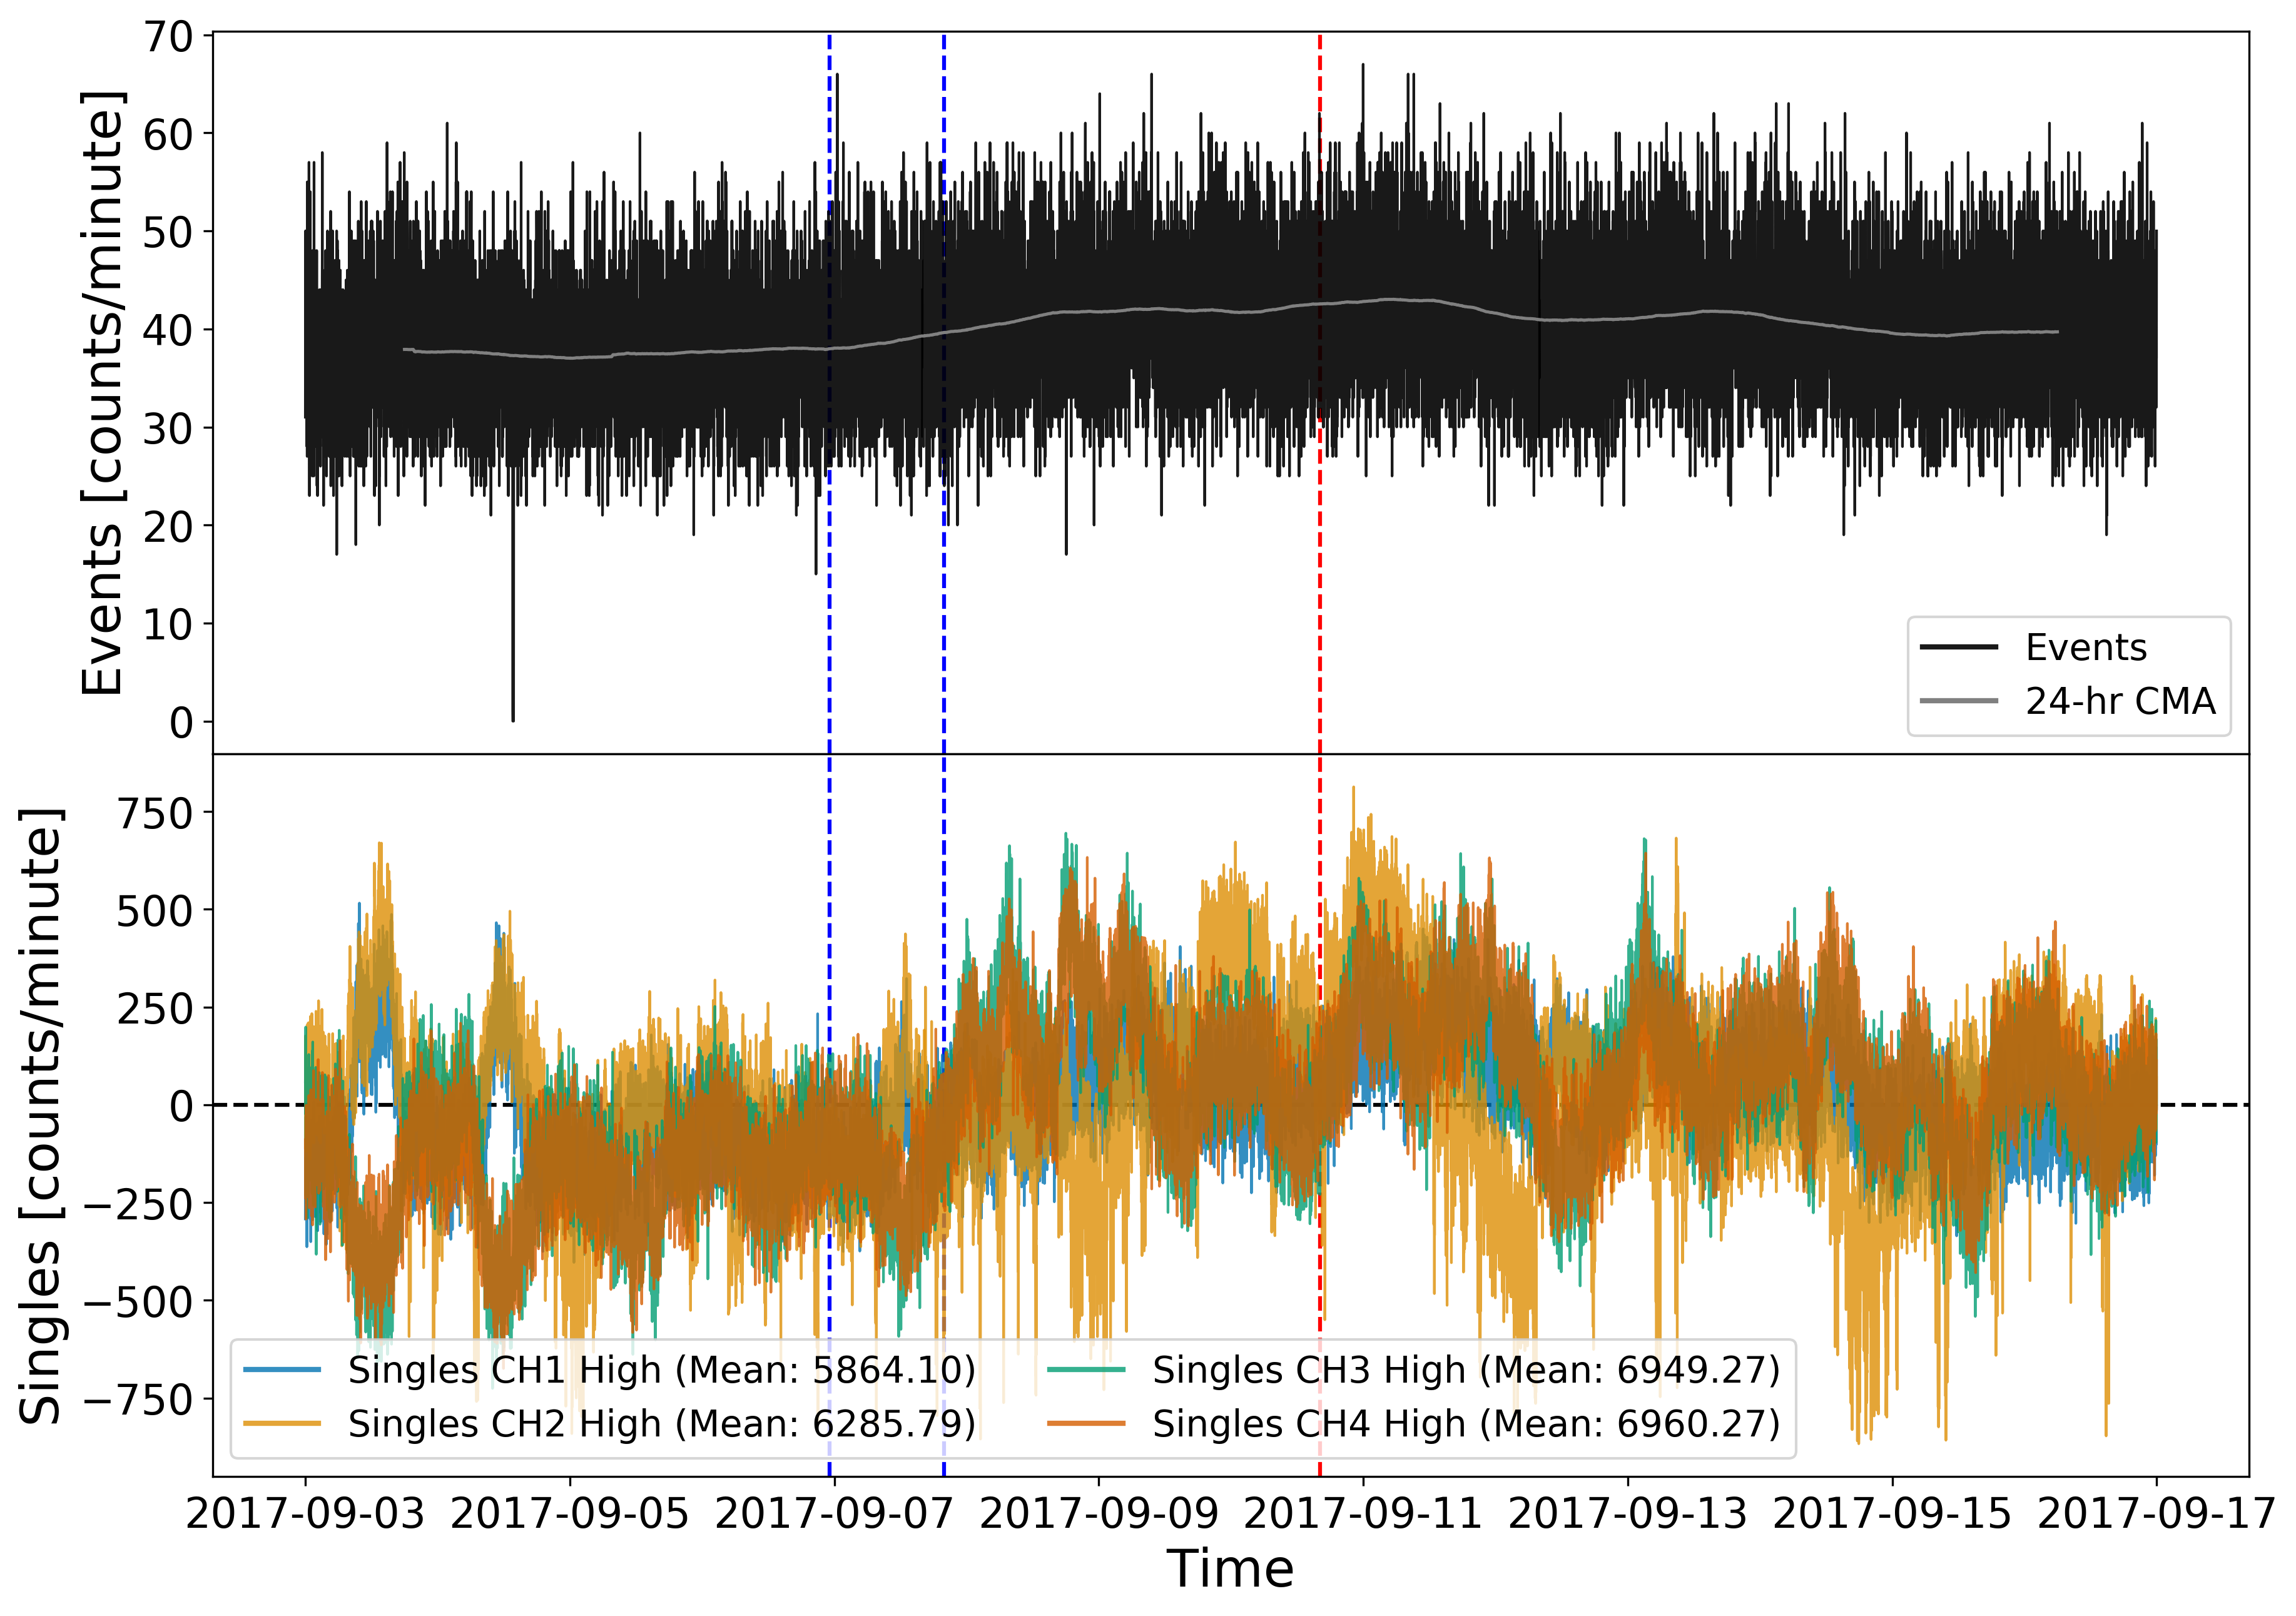
\includegraphics[width=0.48\columnwidth]{FD_GLE72_501.png}
		\label{fig:FD_GLE72_501}}
	%\qquad
	\subfloat[HS 203 (College Hageveld)]{
		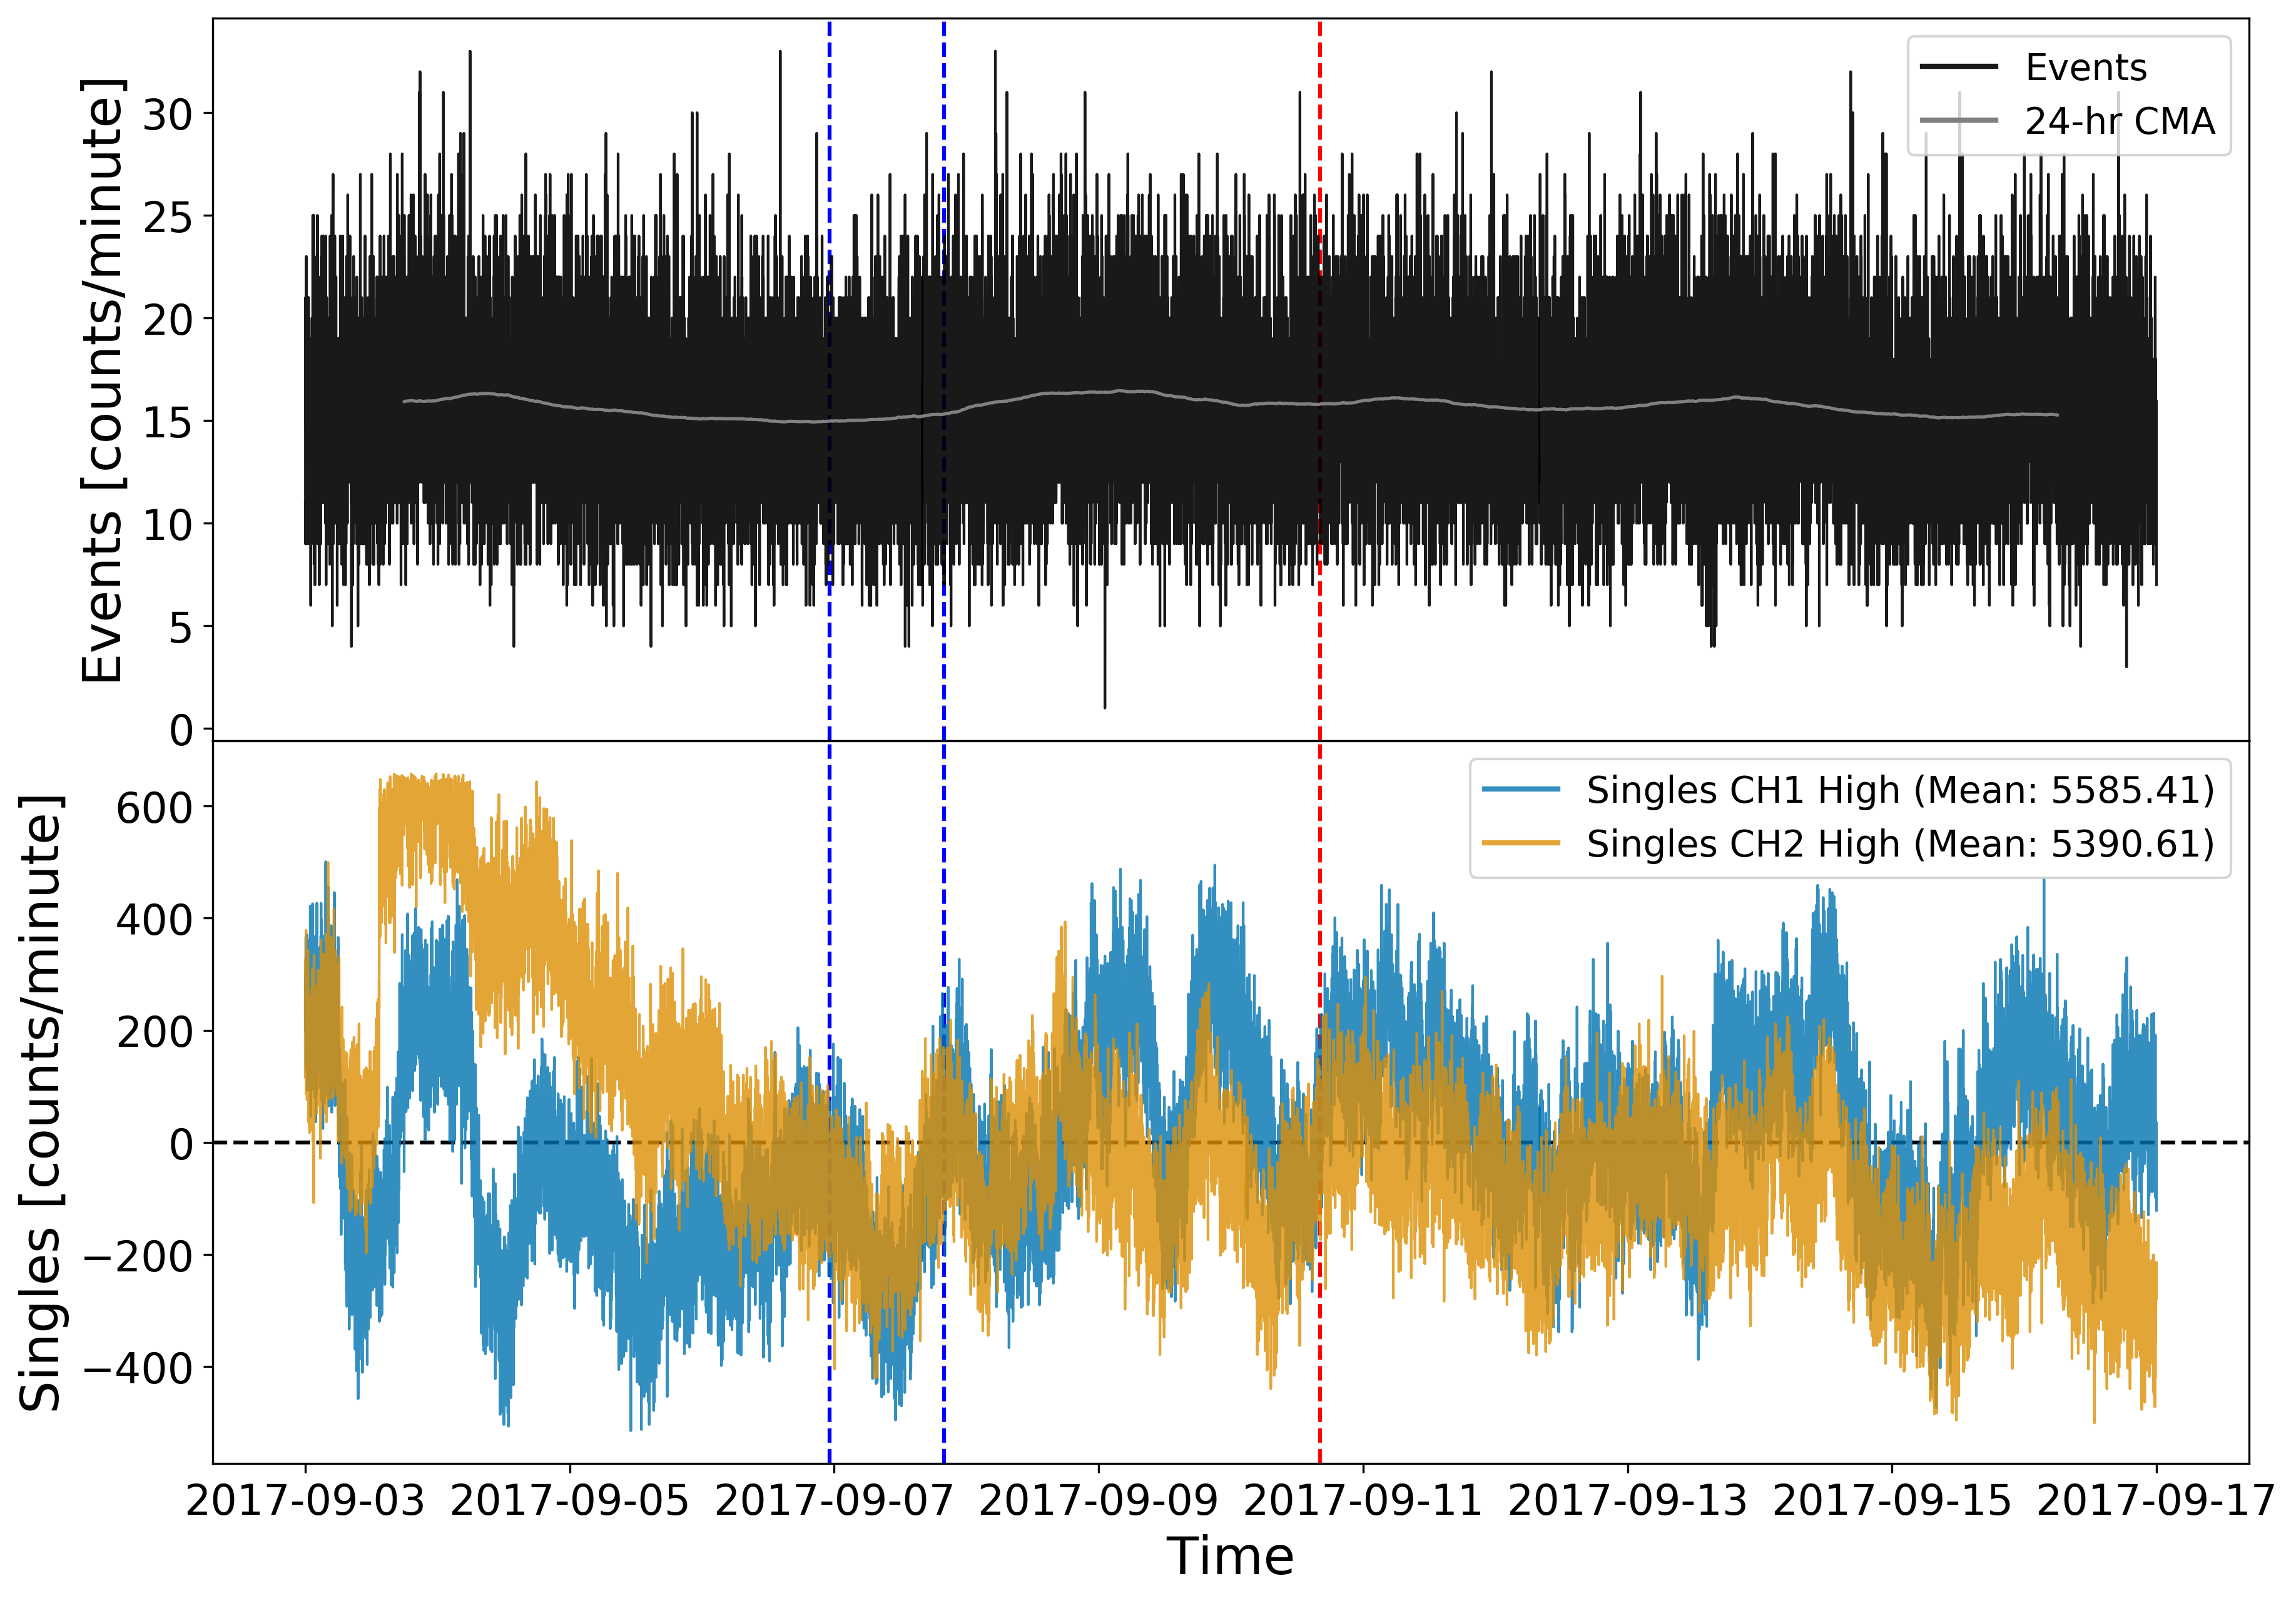
\includegraphics[width=0.48\columnwidth]{FD_GLE72_203.png}
		\label{fig:FD_GLE72_203}} \\
	
	\qquad
	
	\subfloat[HS 8001 (Eindhoven)]{
		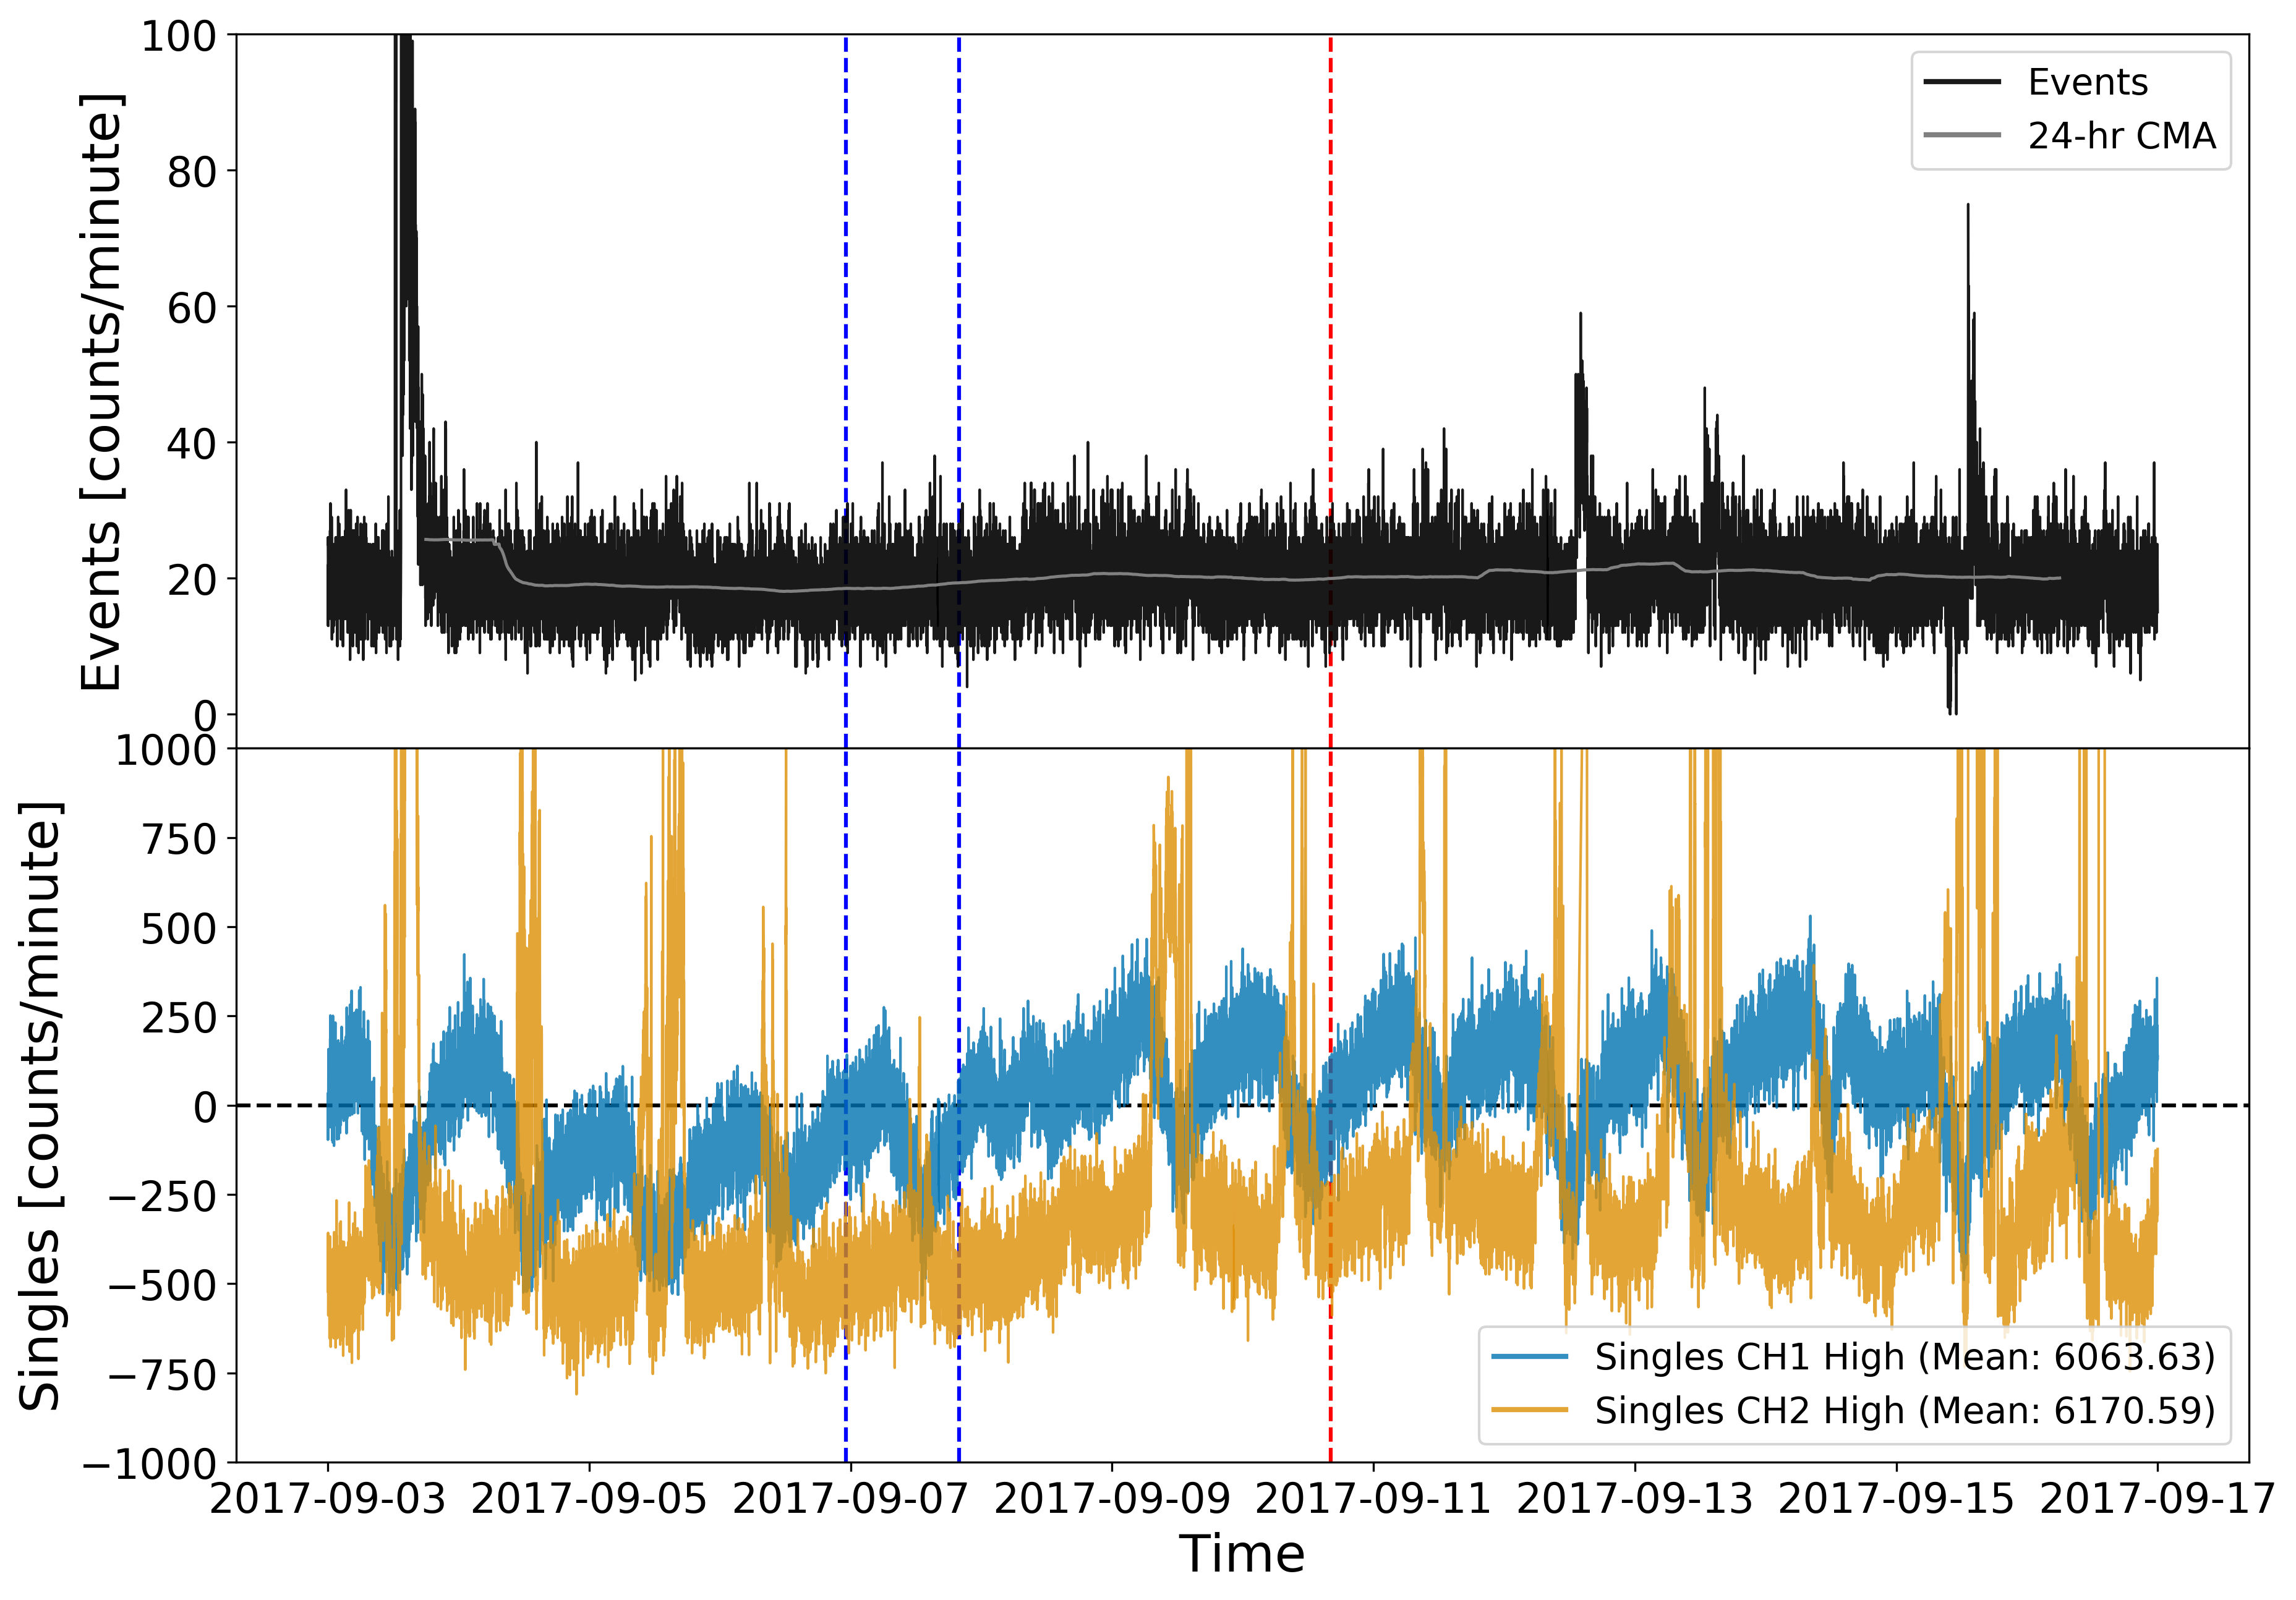
\includegraphics[width=0.48\columnwidth]{FD_GLE72_8001.png}
		\label{fig:FD_GLE72_8001}}
	%\qquad
	\subfloat[HS 14001 (Birmingham University)]{
		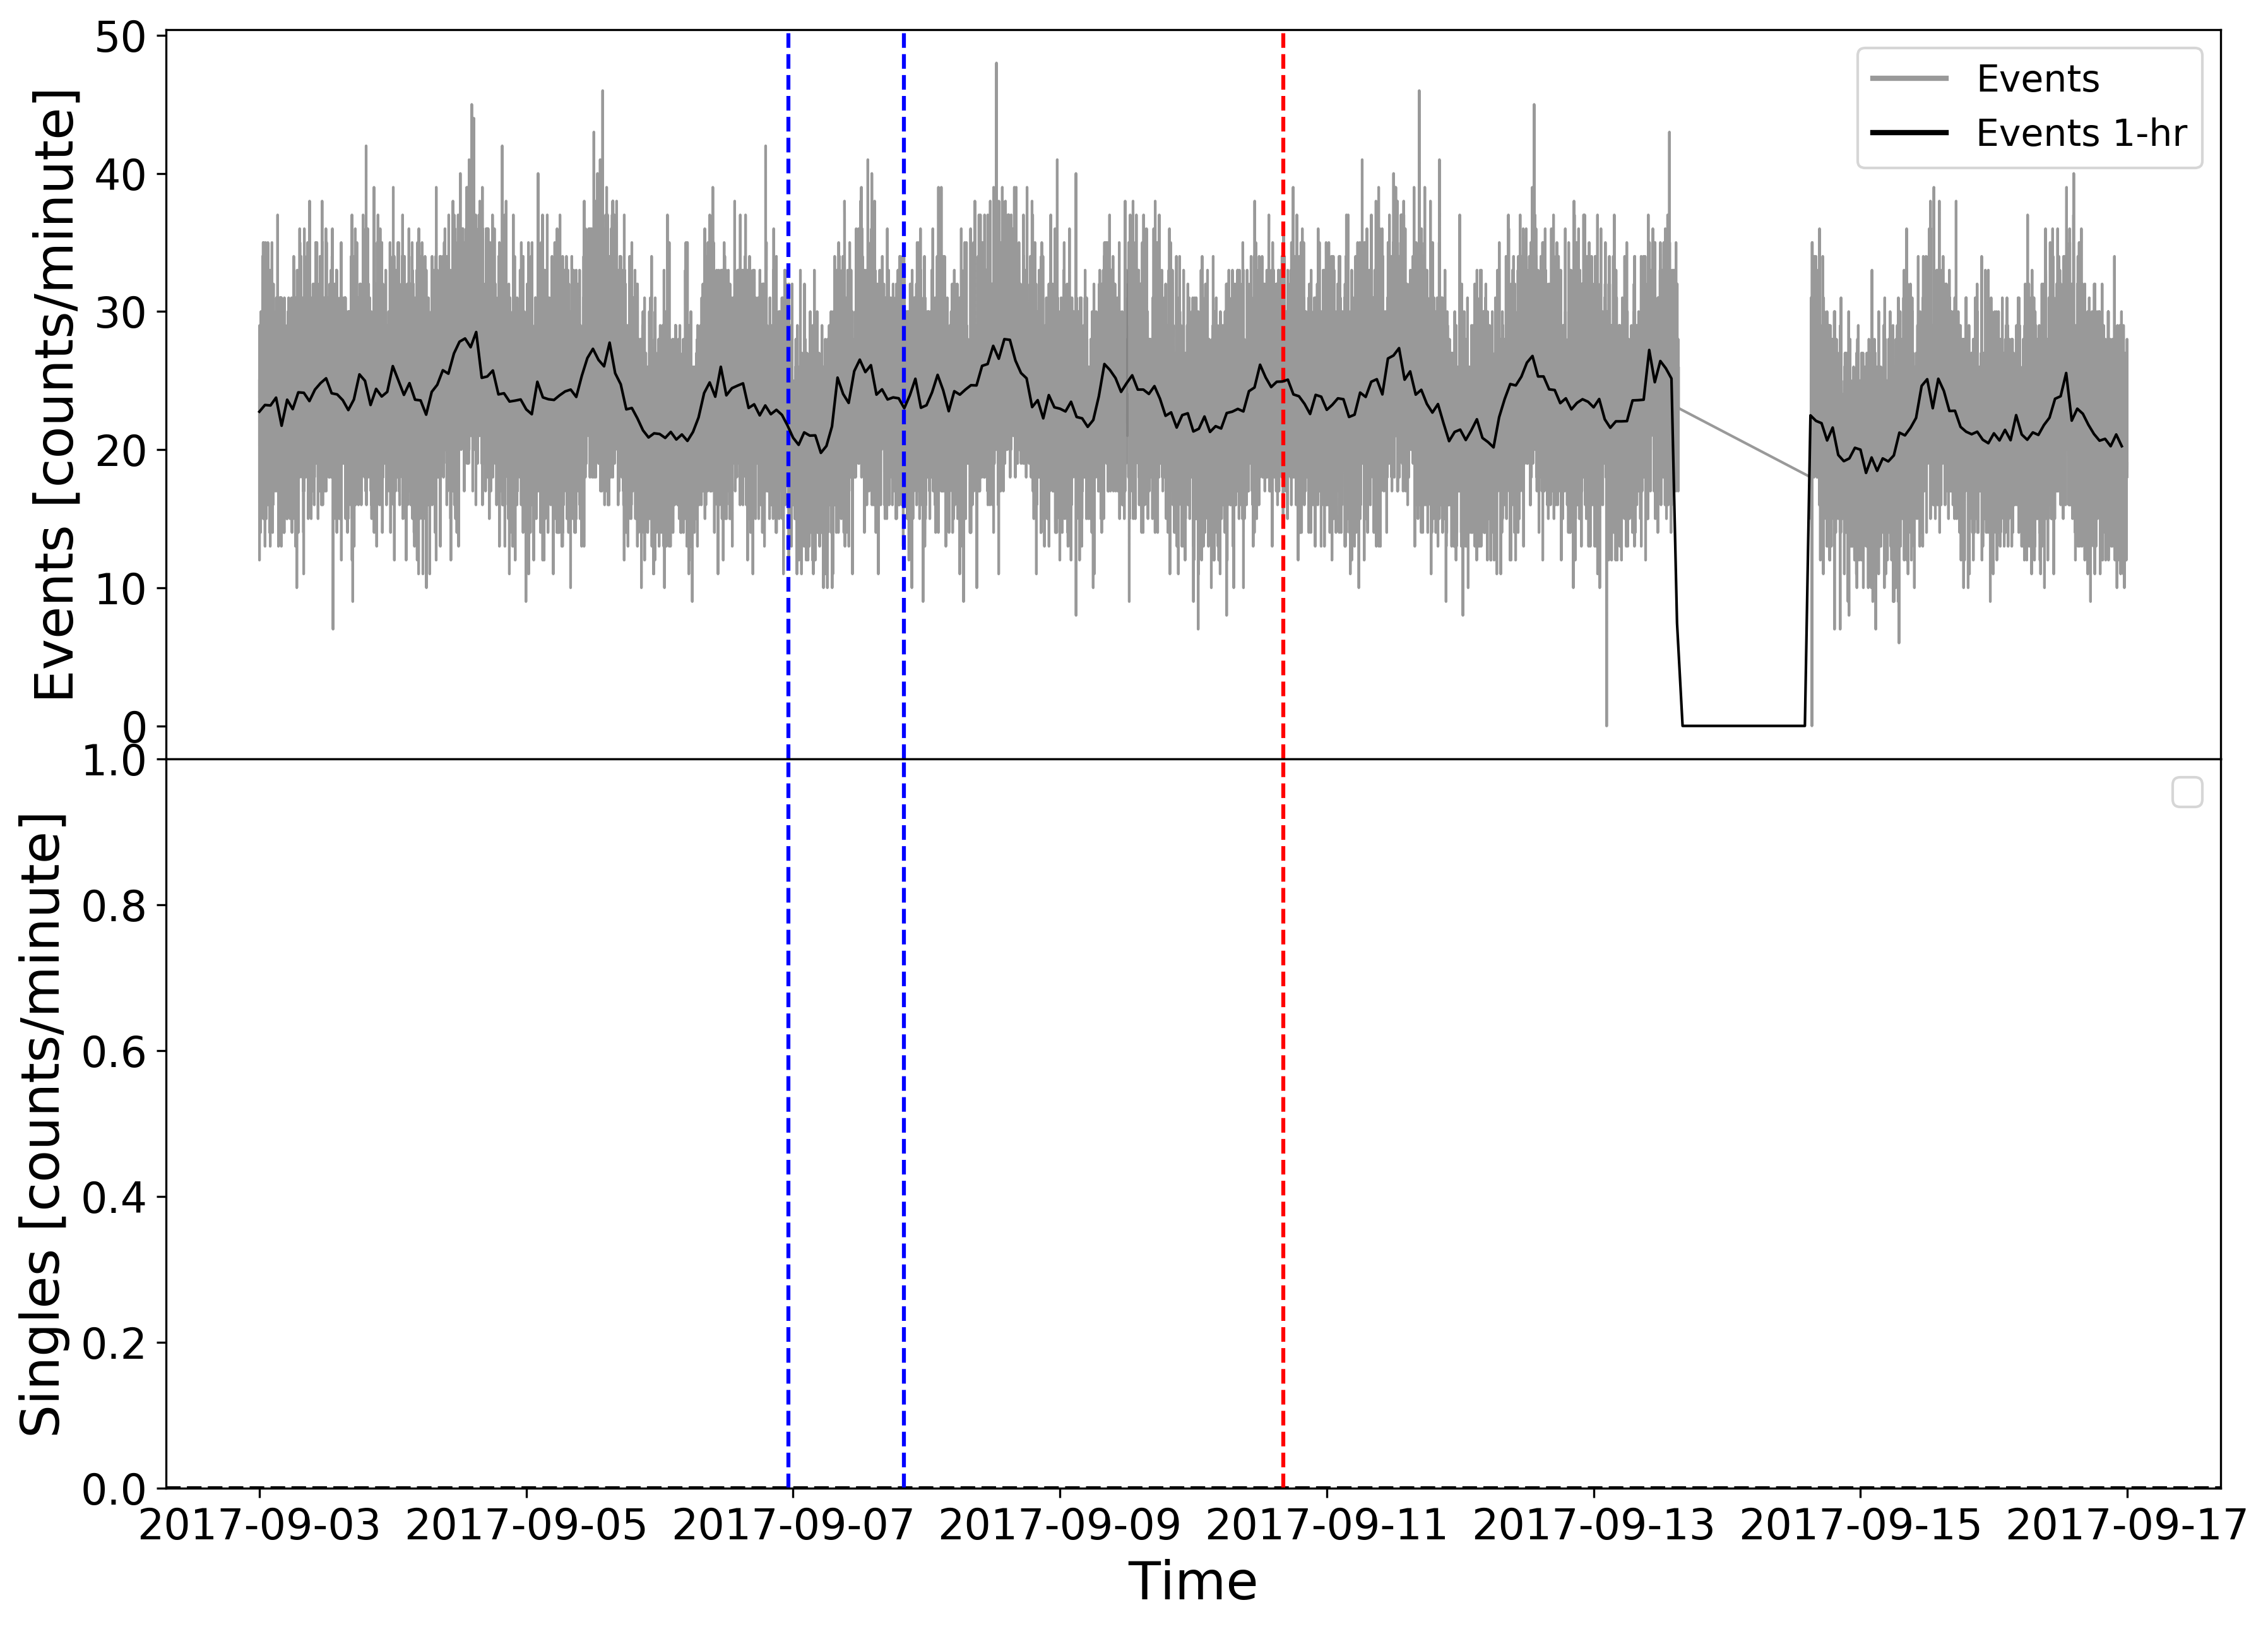
\includegraphics[width=0.48\columnwidth]{FD_GLE72_14001.png}
		\label{fig:FD_GLE72_14001}}
	
	\caption{HiSPARC data for [n] stations around the epoch in which there were several FDs close to the onset of GLE 72. The top panel of each subplot shows the minute-averaged trigger events between detectors within the station, while the bottom panel shows the mean-shifted, minute-averaged counts by each individual detector in the station. The vertical blue-dashed lines show the approximate onset-times of the two FDs observed around this epoch and the red-dashed line depicts the approximate onset time of the GLE.}
	\label{fig:FD_GLE72}
\end{figure}

... no clear FDs seen...



%%%%%%%%%%%%%%%%%%%%%%%%%%%%%%%%%%%%%%%%%%%%%%%%%%%%%%%%%%%%%%%%%%%%%
%%%%%%%%%%%%%%%%%%%%%%%%%%%%%%%%%%%%%%%%%%%%%%%%%%%%%%%%%%%%%%%%%%%%%
\section{Air Shower Simulations}\label{sec:CORSIKA}

In order to understand the footprint of air showers produced by PCRs, simulations of air showers were performed for a range of primary proton and $\alpha$-particle energies.

To simulate the CR air shower development, we employ CORSIKA ({\bf CO}smic {\bf R}ay {\bf SI}mulations for {\bf KA}scade), a Monte Carlo programme providing detailed simulations of the evolution of air showers initiated by cosmic rays particles through the atmosphere \citep{heck_extensive_2017}. The particles in the CORSIKA simulations are tracked through the atmosphere until they undergo interactions with atmospheric nuclei, decay due to their instability, or reach the ground level defined as the end of the simulation.

Proton and $\alpha$-particle initiated air showers were generated with energies ranging from $10^{9}$ to $10^{20}$~eV, and $4\times10^{9}$ to $10^{20}$~eV, respectively. In total $\sim 230000$ proton-initiated showers were simulated and $\sim 180000$ $\alpha$-particle-initiated air showers were simulated. The list of simulated air shower PCRs is shown in Table~\ref{tab:CORSIKA_sims}. For high energy, inelastic hadronic interactions within CORSIKA the QGSJET-II [REF] model was selected. Interactions of hadrons with energies below 80 GeV are simulated using GHEISHA [REF], which allowed for the simulation of PCRs in the regime of SCRs. In addition to these hadronic interactions, electromagnetic interactions within the CORSIKA simulations were described by the EGS4 [REF] model. Furthermore CORSIKA has a minimum muon energy limit that can be simulated of 10 MeV.

\begin{table}
	\begin{center}
	\caption{PCRs simulated using CORSIKA.}
	\label{tab:CORSIKA_sims}
	\begin{tabular}{l r l r | l r l r}
		\hline
		\multicolumn{4}{c}{\bf Protons}  & \multicolumn{4}{c}{\textbf{ $\bm{\alpha}$-Particles}}         \\
		    &    &    &    &    &    &    &    \\
		{\bf E$\bm{_{\mathrm{PCR}}}$ (eV)} & {\bf N$\bm{_{\mathrm{sims}}}$} & {\bf E$\bm{_{\mathrm{PCR}}}$ (eV)} & {\bf N$\bm{_{\mathrm{sims}}}$} & {\bf E$\bm{_{\mathrm{PCR}}}$ (eV)} & {\bf N$\bm{_{\mathrm{sims}}}$} & {\bf E$\bm{_{\mathrm{PCR}}}$ (eV)} & {\bf N$\bm{_{\mathrm{sims}}}$} \\
		\hline
		1.00E+09    & 10000   & 2.98E+12    & 1000    & 4.00E+09    & 10000   & 1.00E+13    & 1000    \\
		1.27E+09    & 10000   & 3.79E+12    & 1000    & 4.28E+09    & 10000   & 1.78E+13    & 100     \\
		1.62E+09    & 10000   & 4.83E+12    & 1000    & 5.46E+09    & 10000   & 3.16E+13    & 100     \\
		2.07E+09    & 10000   & 6.16E+12    & 1000    & 6.95E+09    & 10000   & 5.62E+13    & 100     \\
		2.64E+09    & 10000   & 7.85E+12    & 1000    & 8.86E+09    & 10000   & 1.00E+14    & 100     \\
		3.36E+09    & 10000   & 1.00E+13    & 1000    & 1.00E+10    & 10000   & 1.78E+14    & 50      \\
		4.28E+09    & 10000   & 1.78E+13    & 100     & 1.13E+10    & 10000   & 3.16E+14    & 50      \\
		5.46E+09    & 10000   & 3.16E+13    & 100     & 1.44E+10    & 10000   & 5.62E+14    & 50      \\
		6.95E+09    & 10000   & 5.62E+13    & 100     & 1.83E+10    & 10000   & 1.00E+15    & 10      \\
		8.86E+09    & 10000   & 1.00E+14    & 100     & 2.34E+10    & 10000   & 1.78E+15    & 10      \\
		1.00E+10    & 10000   & 1.78E+14    & 50      & 2.98E+10    & 10000   & 3.16E+15    & 10      \\
		1.13E+10    & 10000   & 3.16E+14    & 50      & 3.79E+10    & 10000   & 5.62E+15    & 10      \\
		1.44E+10    & 10000   & 5.62E+14    & 50      & 4.83E+10    & 10000   & 1.00E+16    & 10      \\
		1.83E+10    & 10000   & 1.00E+15    & 10      & 6.16E+10    & 10000   & 1.78E+16    & 10      \\
		2.34E+10    & 10000   & 1.78E+15    & 10      & 7.85E+10    & 10000   & 3.16E+16    & 10      \\
		2.98E+10    & 10000   & 3.16E+15    & 10      & 1.00E+11    & 10000   & 5.62E+16    & 10      \\
		3.79E+10    & 10000   & 5.62E+15    & 10      & 1.27E+11    & 1000    & 1.00E+17    & 10      \\
		4.83E+10    & 10000   & 1.00E+16    & 10      & 1.62E+11    & 1000    & 1.78E+17    & 10      \\
		6.16E+10    & 10000   & 1.78E+16    & 10      & 2.07E+11    & 1000    & 3.16E+17    & 10      \\
		7.85E+10    & 10000   & 3.16E+16    & 10      & 2.64E+11    & 1000    & 5.62E+17    & 10      \\
		1.00E+11    & 10000   & 5.62E+16    & 10      & 3.36E+11    & 1000    & 1.00E+18    & 10      \\
		1.27E+11    & 1000    & 1.00E+17    & 10      & 4.28E+11    & 1000    & 1.78E+18    & 10      \\
		1.62E+11    & 1000    & 1.78E+17    & 10      & 5.46E+11    & 1000    & 3.16E+18    & 10      \\
		2.07E+11    & 1000    & 3.16E+17    & 10      & 6.95E+11    & 1000    & 5.62E+18    & 10      \\
		2.64E+11    & 1000    & 5.62E+17    & 10      & 8.86E+11    & 1000    & 1.00E+19    & 10      \\
		3.36E+11    & 1000    & 1.00E+18    & 10      & 1.13E+12    & 1000    & 1.78E+19    & 10      \\
		4.28E+11    & 1000    & 1.78E+18    & 10      & 1.44E+12    & 1000    & 3.16E+19    & 10      \\
		5.46E+11    & 1000    & 3.16E+18    & 10      & 1.83E+12    & 1000    & 5.62E+19    & 10      \\
		6.95E+11    & 1000    & 5.62E+18    & 10      & 2.34E+12    & 1000    & 1.00E+20    & 10      \\
		8.86E+11    & 1000    & 1.00E+19    & 10      & 2.98E+12    & 1000    &             &         \\
		1.13E+12    & 1000    & 1.78E+19    & 10      & 3.79E+12    & 1000    &             &         \\
		1.44E+12    & 1000    & 3.16E+19    & 10      & 4.83E+12    & 1000    &             &         \\
		1.83E+12    & 1000    & 5.62E+19    & 10      & 6.16E+12    & 1000    &             &         \\
		2.34E+12    & 1000    & 1.00E+20    & 10      & 7.85E+12    & 1000    &             &         \\   
		\hline
	\end{tabular}
	\end{center}
\end{table}

There are several other user-definable setting within CORSIKA which are explained in-depth in the CORSIKA user's guide \citep{heck_extensive_2017}. The settings chosen within these simulation are breifly discussed below. Simulation thinning was enable in CORSIKA to reduce computation time and reduce the output file size. The observation level at which point the simulation cease was set at 100 m above sea level (compared to the $\sim 50$ m typical of the stations, however this difference is negligible for the air shower development.) The pre-defined central European atmosphere in October was used for all simulations, and western-European magnetic field was used as calculated with the \textit{Geomag} programme [REF]: B$_{\mathrm{x}}=18.799$~$\mu$T and B$_{\mathrm{z}}=44.980$~$\mu$T.


%%%%%%%%%%%%%%%%%%%%%%%%%%%%%%%%%%%%%%%%%%%%%%%%%%%%%%%%%%%%%%%%%%%%%
\subsection{Air Shower Footprints}\label{sec:CORSIKA_footprint}

The average footprint of muons at ground level was acquired from the output CORSIKA simulations. This was achieved by simply taking the distributino of the muons at ground level at the end of the simulation as a function of their distance from the shower core for each individual simulation realisation. For a given PCR energy the average air shower footprint distribution is calculated by combining the individual simulation realisations.

%[Discuss how distance between the HiSPARC station 2d/4d detectors will impact the ability to view certain PCR energies, and sets an lower limit on the energies observable in the standard trigger mode]

\begin{figure}
	\centering
	\subfloat[Proton initiated air shower. \label{fig:p_footprint}]{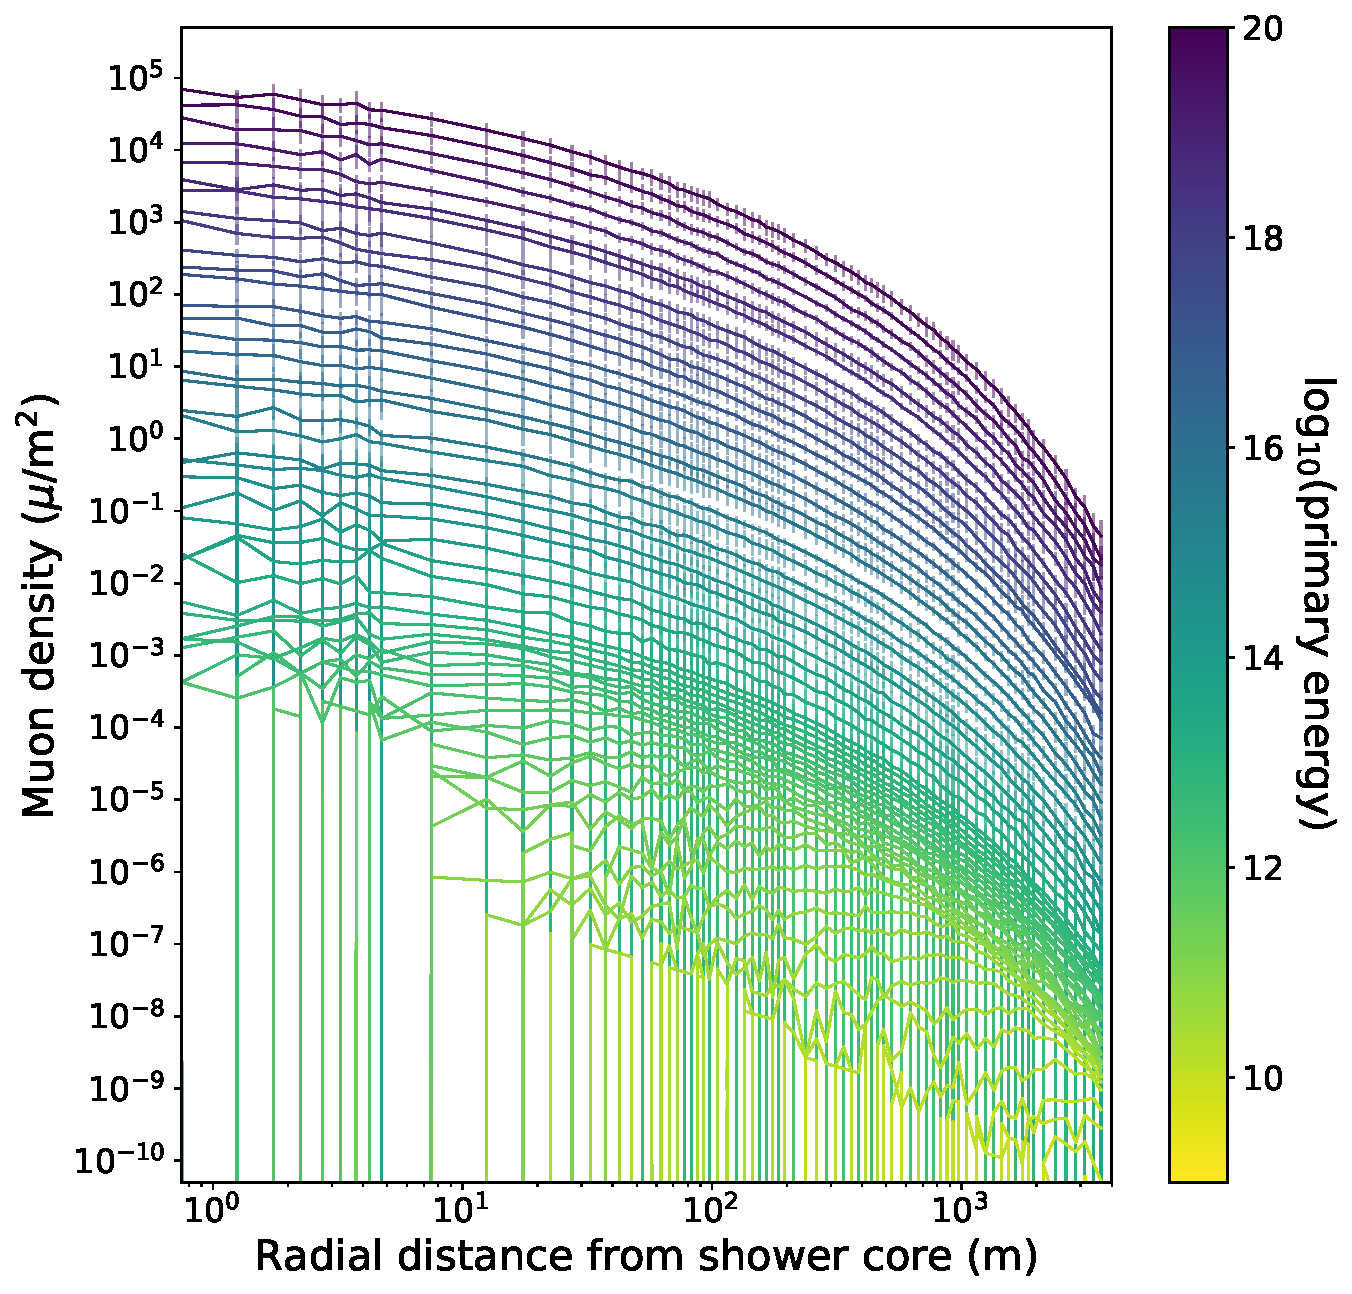
\includegraphics[width=0.47\columnwidth]{proton_footprint.pdf}} 
	\qquad
	\subfloat[$\alpha$-particle initiated air shower. \label{fig:a_footprint}]{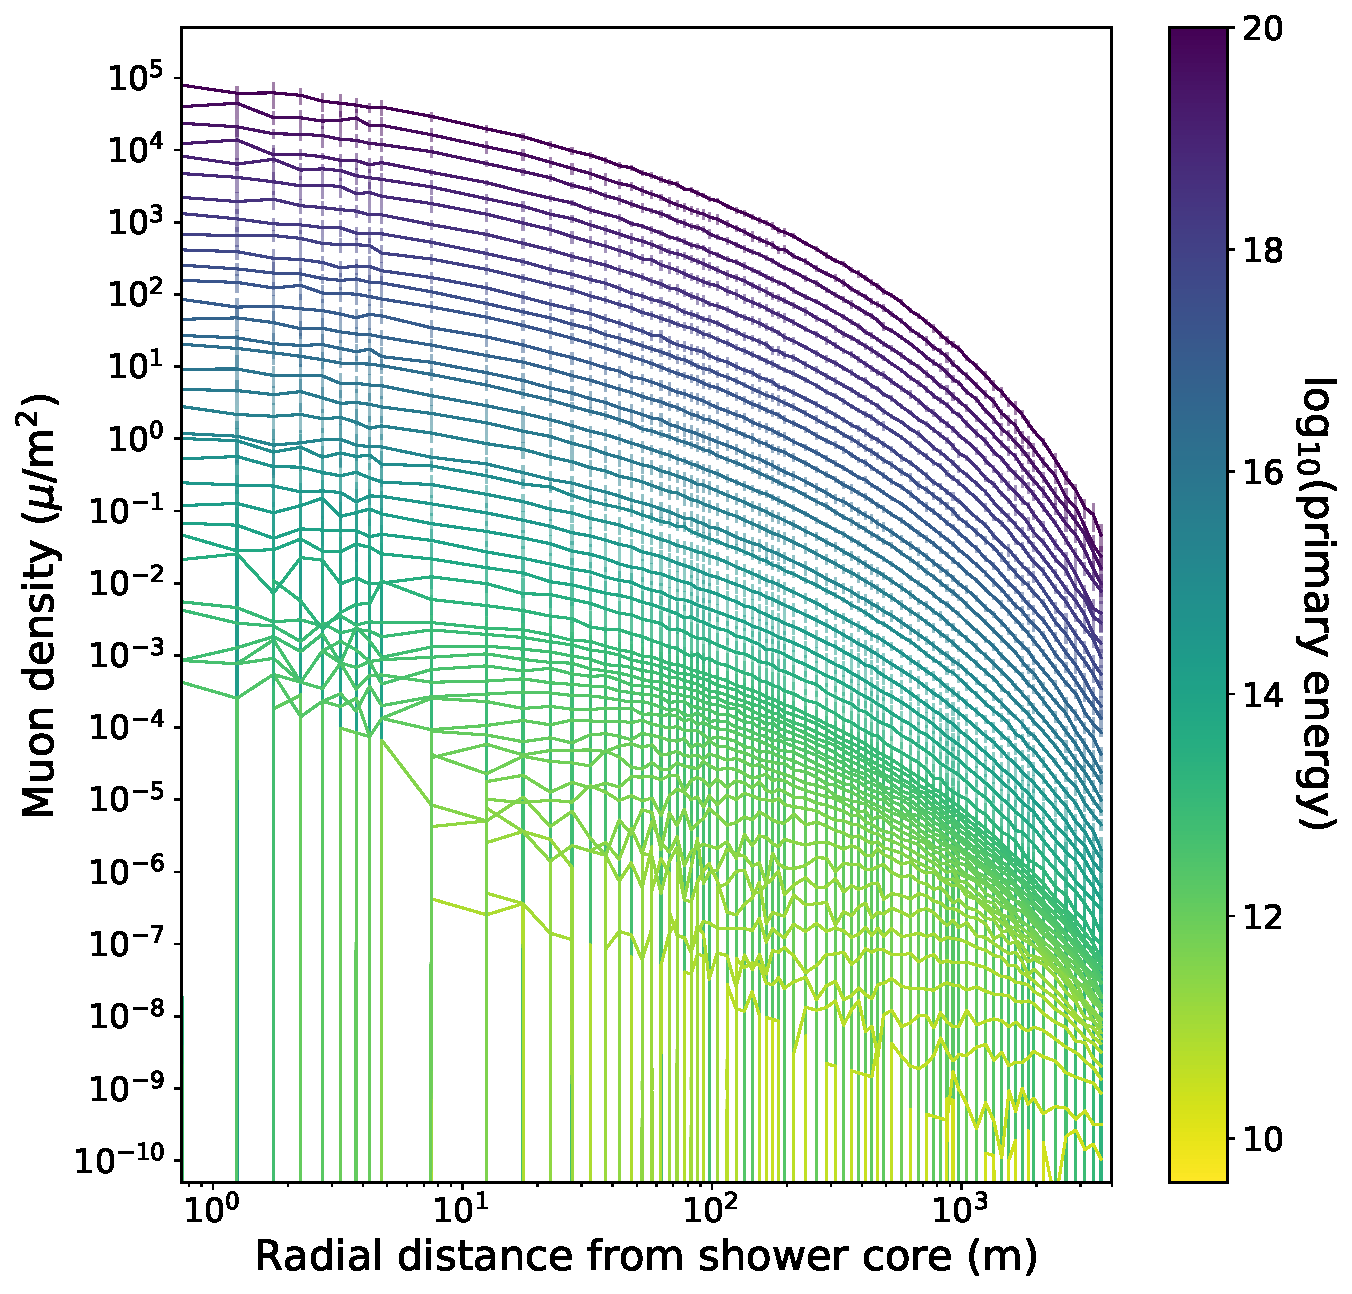
\includegraphics[width=0.47\columnwidth]{alpha_footprint.pdf}}
	\caption{Mean muon density footprints for (a) proton-initiated air showers and (b) $\alpha$-particle-initiated air showers with intial PCR trajectories with zenith angles $\theta=0^{\circ}$ and various PCR energies. The error bars given represent 1$\sigma$.} \label{fig:shower_footprints}
\end{figure}

The interpretation of Figure~\ref{fig:shower_footprints} can provide an understanding of the minimum energy of PCRs observable by the different stations within the HiSPARC network. The typical separation between the detectors in a HiSPARC station is $\sim 10$~m, however the separation between detectors can be up to as much as 20~m or as low as a couple of metres. This analysis of the air shower footprint shows the variation in PCR energy sampled varies marginally over this range of distances and suggests that HiSPARC stations will typical observe PCR with an energy of $\sim 10^{14}-10^{15}$~eV to meet the required trigger conditions.

%\begin{table}
%	\begin{center}
%		\caption{HS station minimum observable PCR energy}
%		\label{tab:footprints}
%		\begin{tabular}{l c c c}
%		\hline
%		{Station ID} & {Average separation (m)} & {Proton E$_{\mathrm{min}}$} & {$\alpha$-particle E$_{\mathrm{min}}$} \\
%		\hline
%		{501} & {11.2} & {} & {} \\
%		{14001} & {9.1} & {} & {} \\
%		{} & {} & {} & {} \\
%		\hline
%\end{tabular}
%\end{center}
%\end{table}


\subsection{Muon Flux}\label{sec:CORSIKA_flux}

From the air shower simulations it is possible to gain an estimate of the muon flux at groud-level based on the number of 

\begin{figure}
	\centering
	\subfloat[Proton initiated air shower. \label{fig:p_muons}]{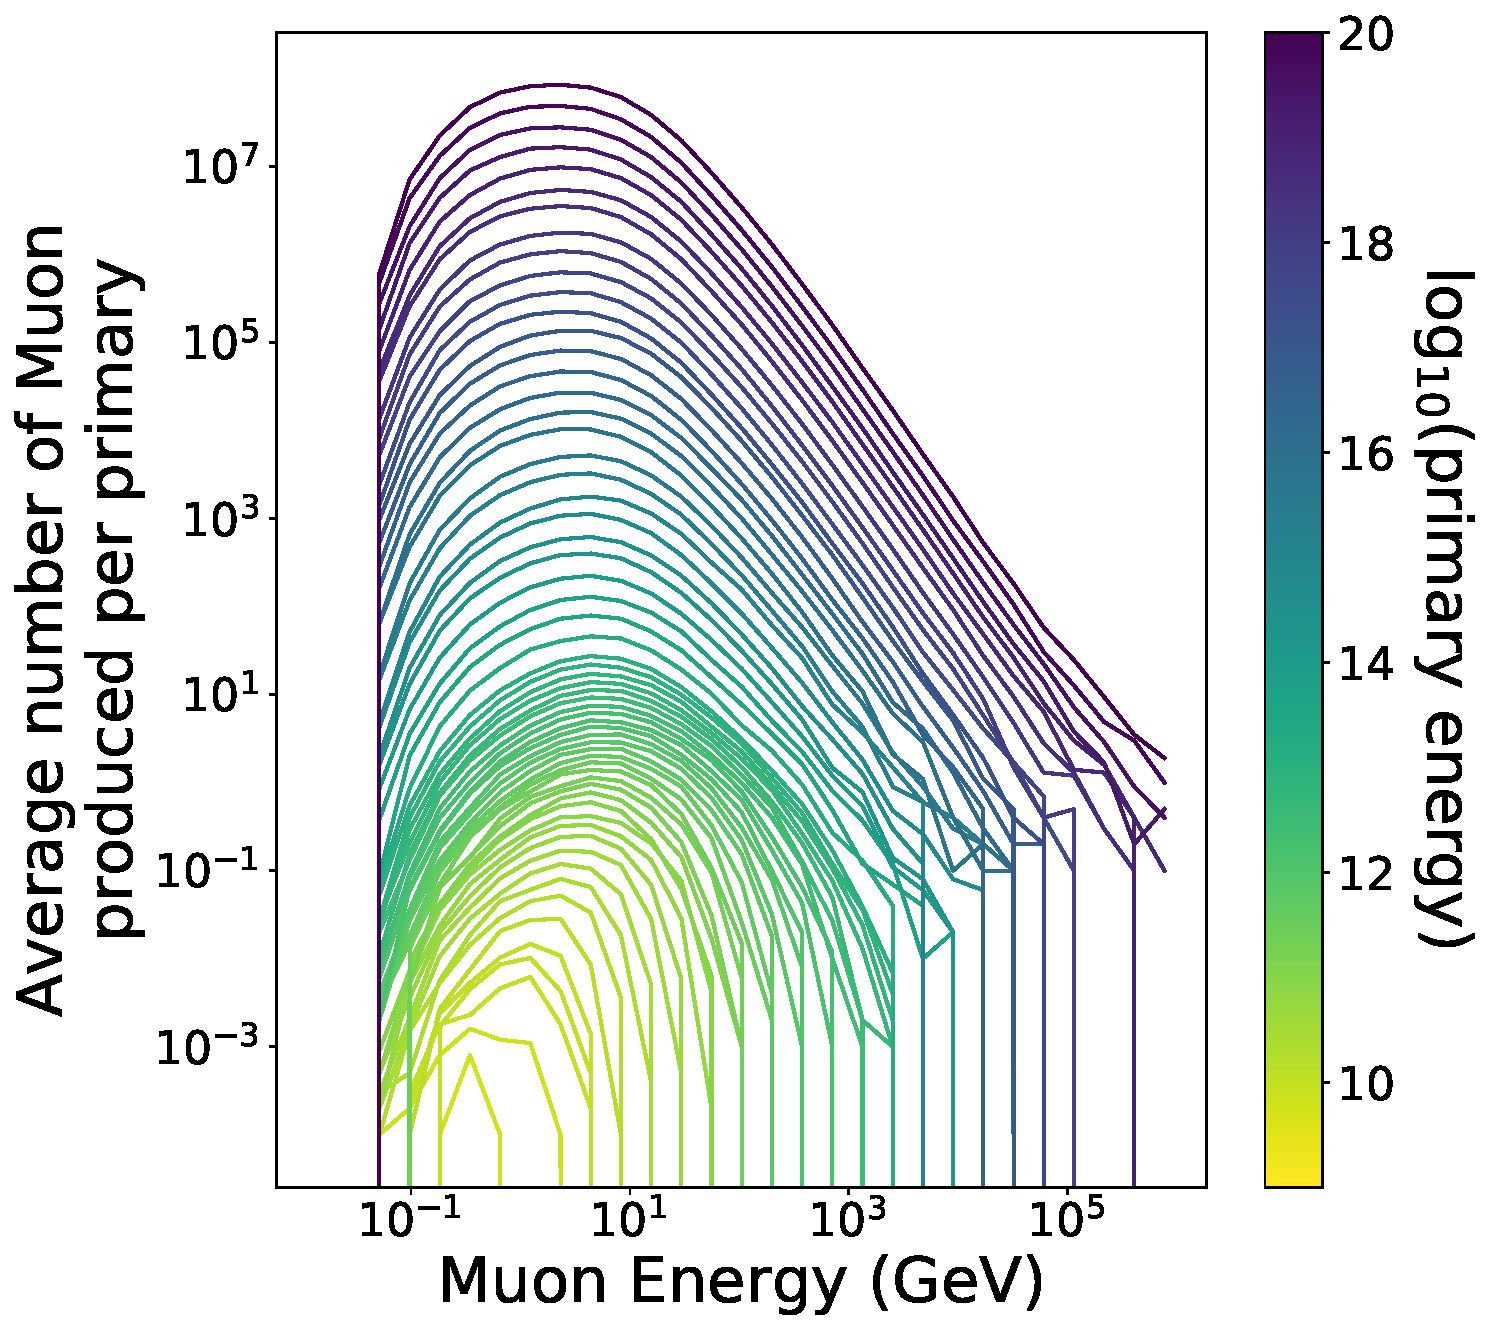
\includegraphics[width=0.47\columnwidth]{proton_muon_number.pdf}} 
	\qquad
	\subfloat[$\alpha$-particle initiated air shower. \label{fig:a_muons}]{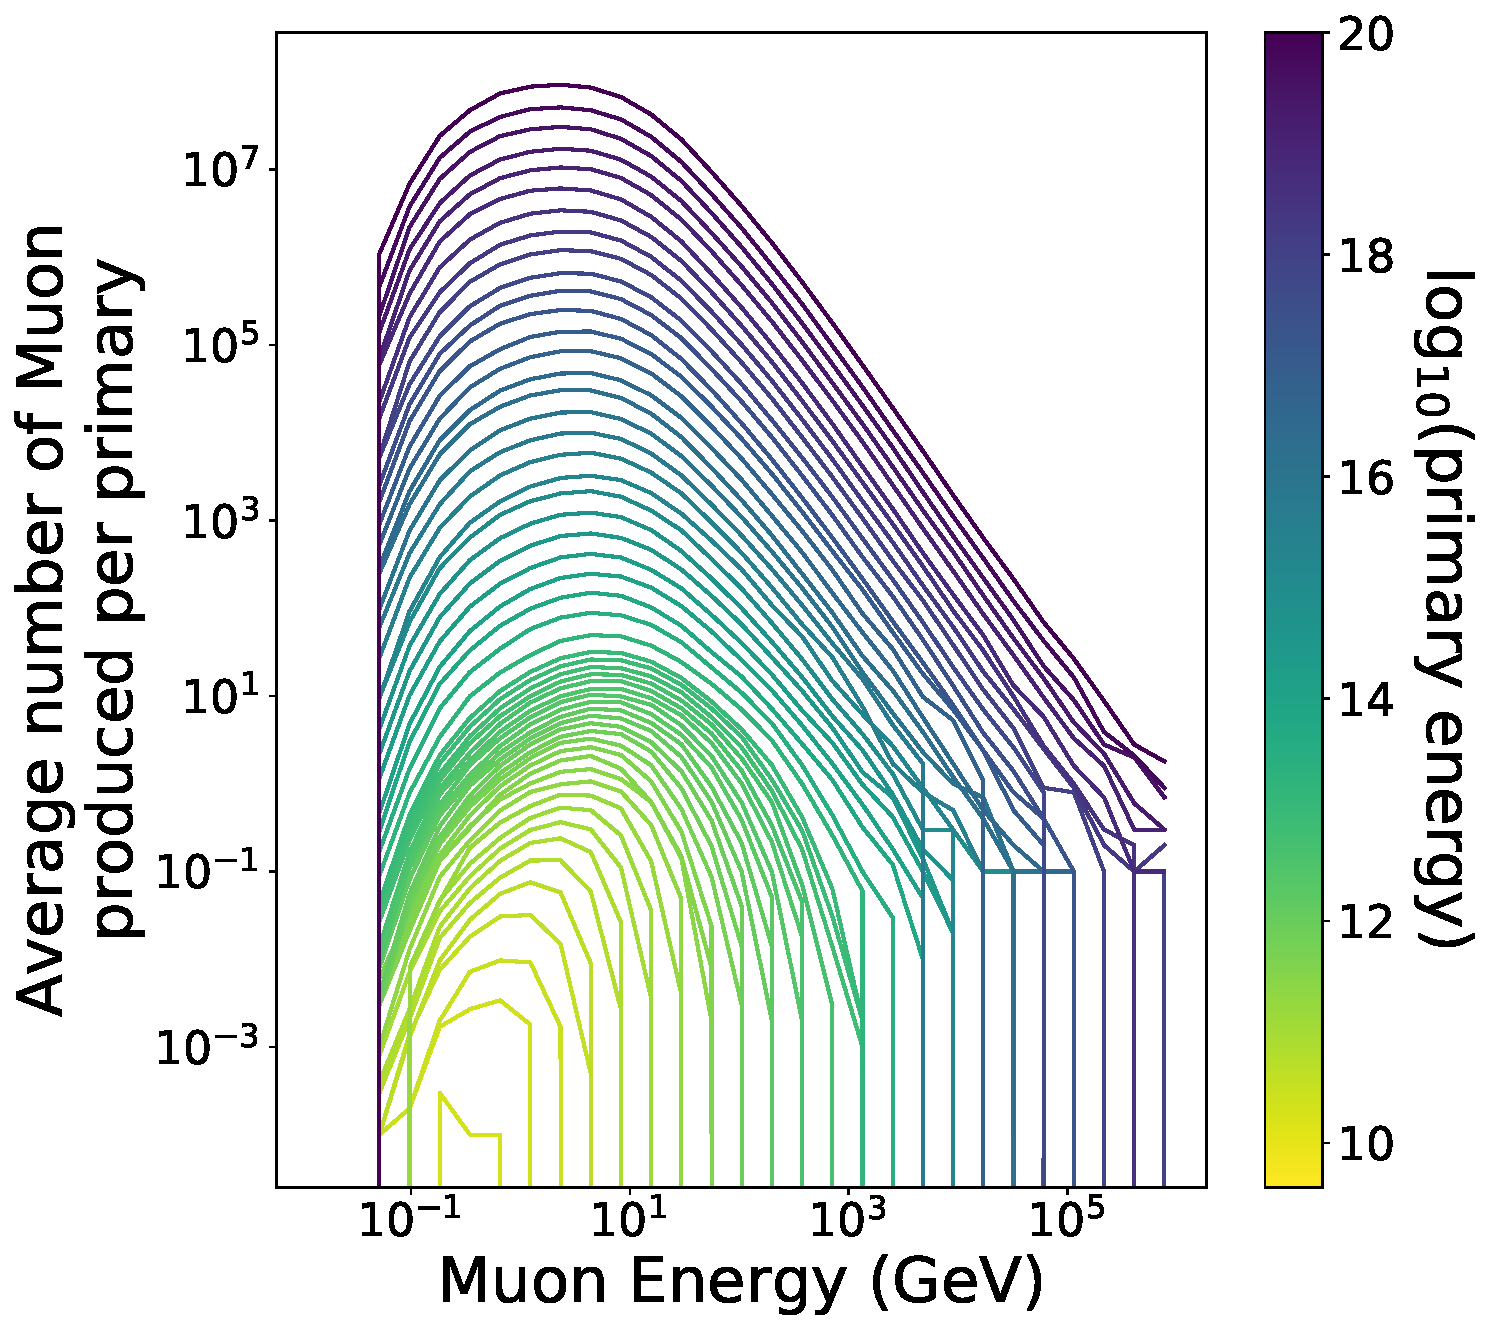
\includegraphics[width=0.47\columnwidth]{alpha_muon_number.pdf}}
	\caption{Mean number of muons produced at ground level by the PCR for (a) proton-initiated air showers and (b) $\alpha$-particle-initiated air showers, for various PCR energy. The uncertainty bars given represent 1$\sigma$.}
	\label{fig:shower_muons}
\end{figure}



%%%%%%%%%%%%%%%%%%%%%%%%%%%%%%%%%%%%%%%%%%%%%%%%%%%%%%%%%%%%%%%%%%%%%
%%%%%%%%%%%%%%%%%%%%%%%%%%%%%%%%%%%%%%%%%%%%%%%%%%%%%%%%%%%%%%%%%%%%%
\section{Standardisation of HiSPARC Data}\label{sec:HS_standardisation}

%%%%%%%%%%%%%%%%%%%%%%%%%%%%%%%%%%%%%%%%%%%%%%%%%%%%%%%%%%%%%%%%%%%%%
\subsection{Motivation}
- HiSPARC stations are individually managed and guidlines aren't stringent
- Variability between stations exists and also apparently between detectors within a station (i.e. see singles during GLE 72)

%%%%%%%%%%%%%%%%%%%%%%%%%%%%%%%%%%%%%%%%%%%%%%%%%%%%%%%%%%%%%%%%%%%%%
\subsection{Barometric Correction}\label{sec:HS_P_corr}

It is understood that observations made by ground-based CR detectors are susceptible to atmospheric conditions. Atmospheric pressure effects the CR travel path due to the expansion and contraction of the atmosphere with varying pressure; hence the CR counts are observed to be negatively correlated to atmospheric pressure as shown for both NMs and MDs in Figure~\ref{fig:CR_V_P}. A correction for this barometric effect is routinely applied as part of the data calibration for all NM stations within the NMDB NEST, but there is no such process in the HiSPARC network.


\begin{figure}[ht]
	\centering
	\subfloat[NM Station]{
		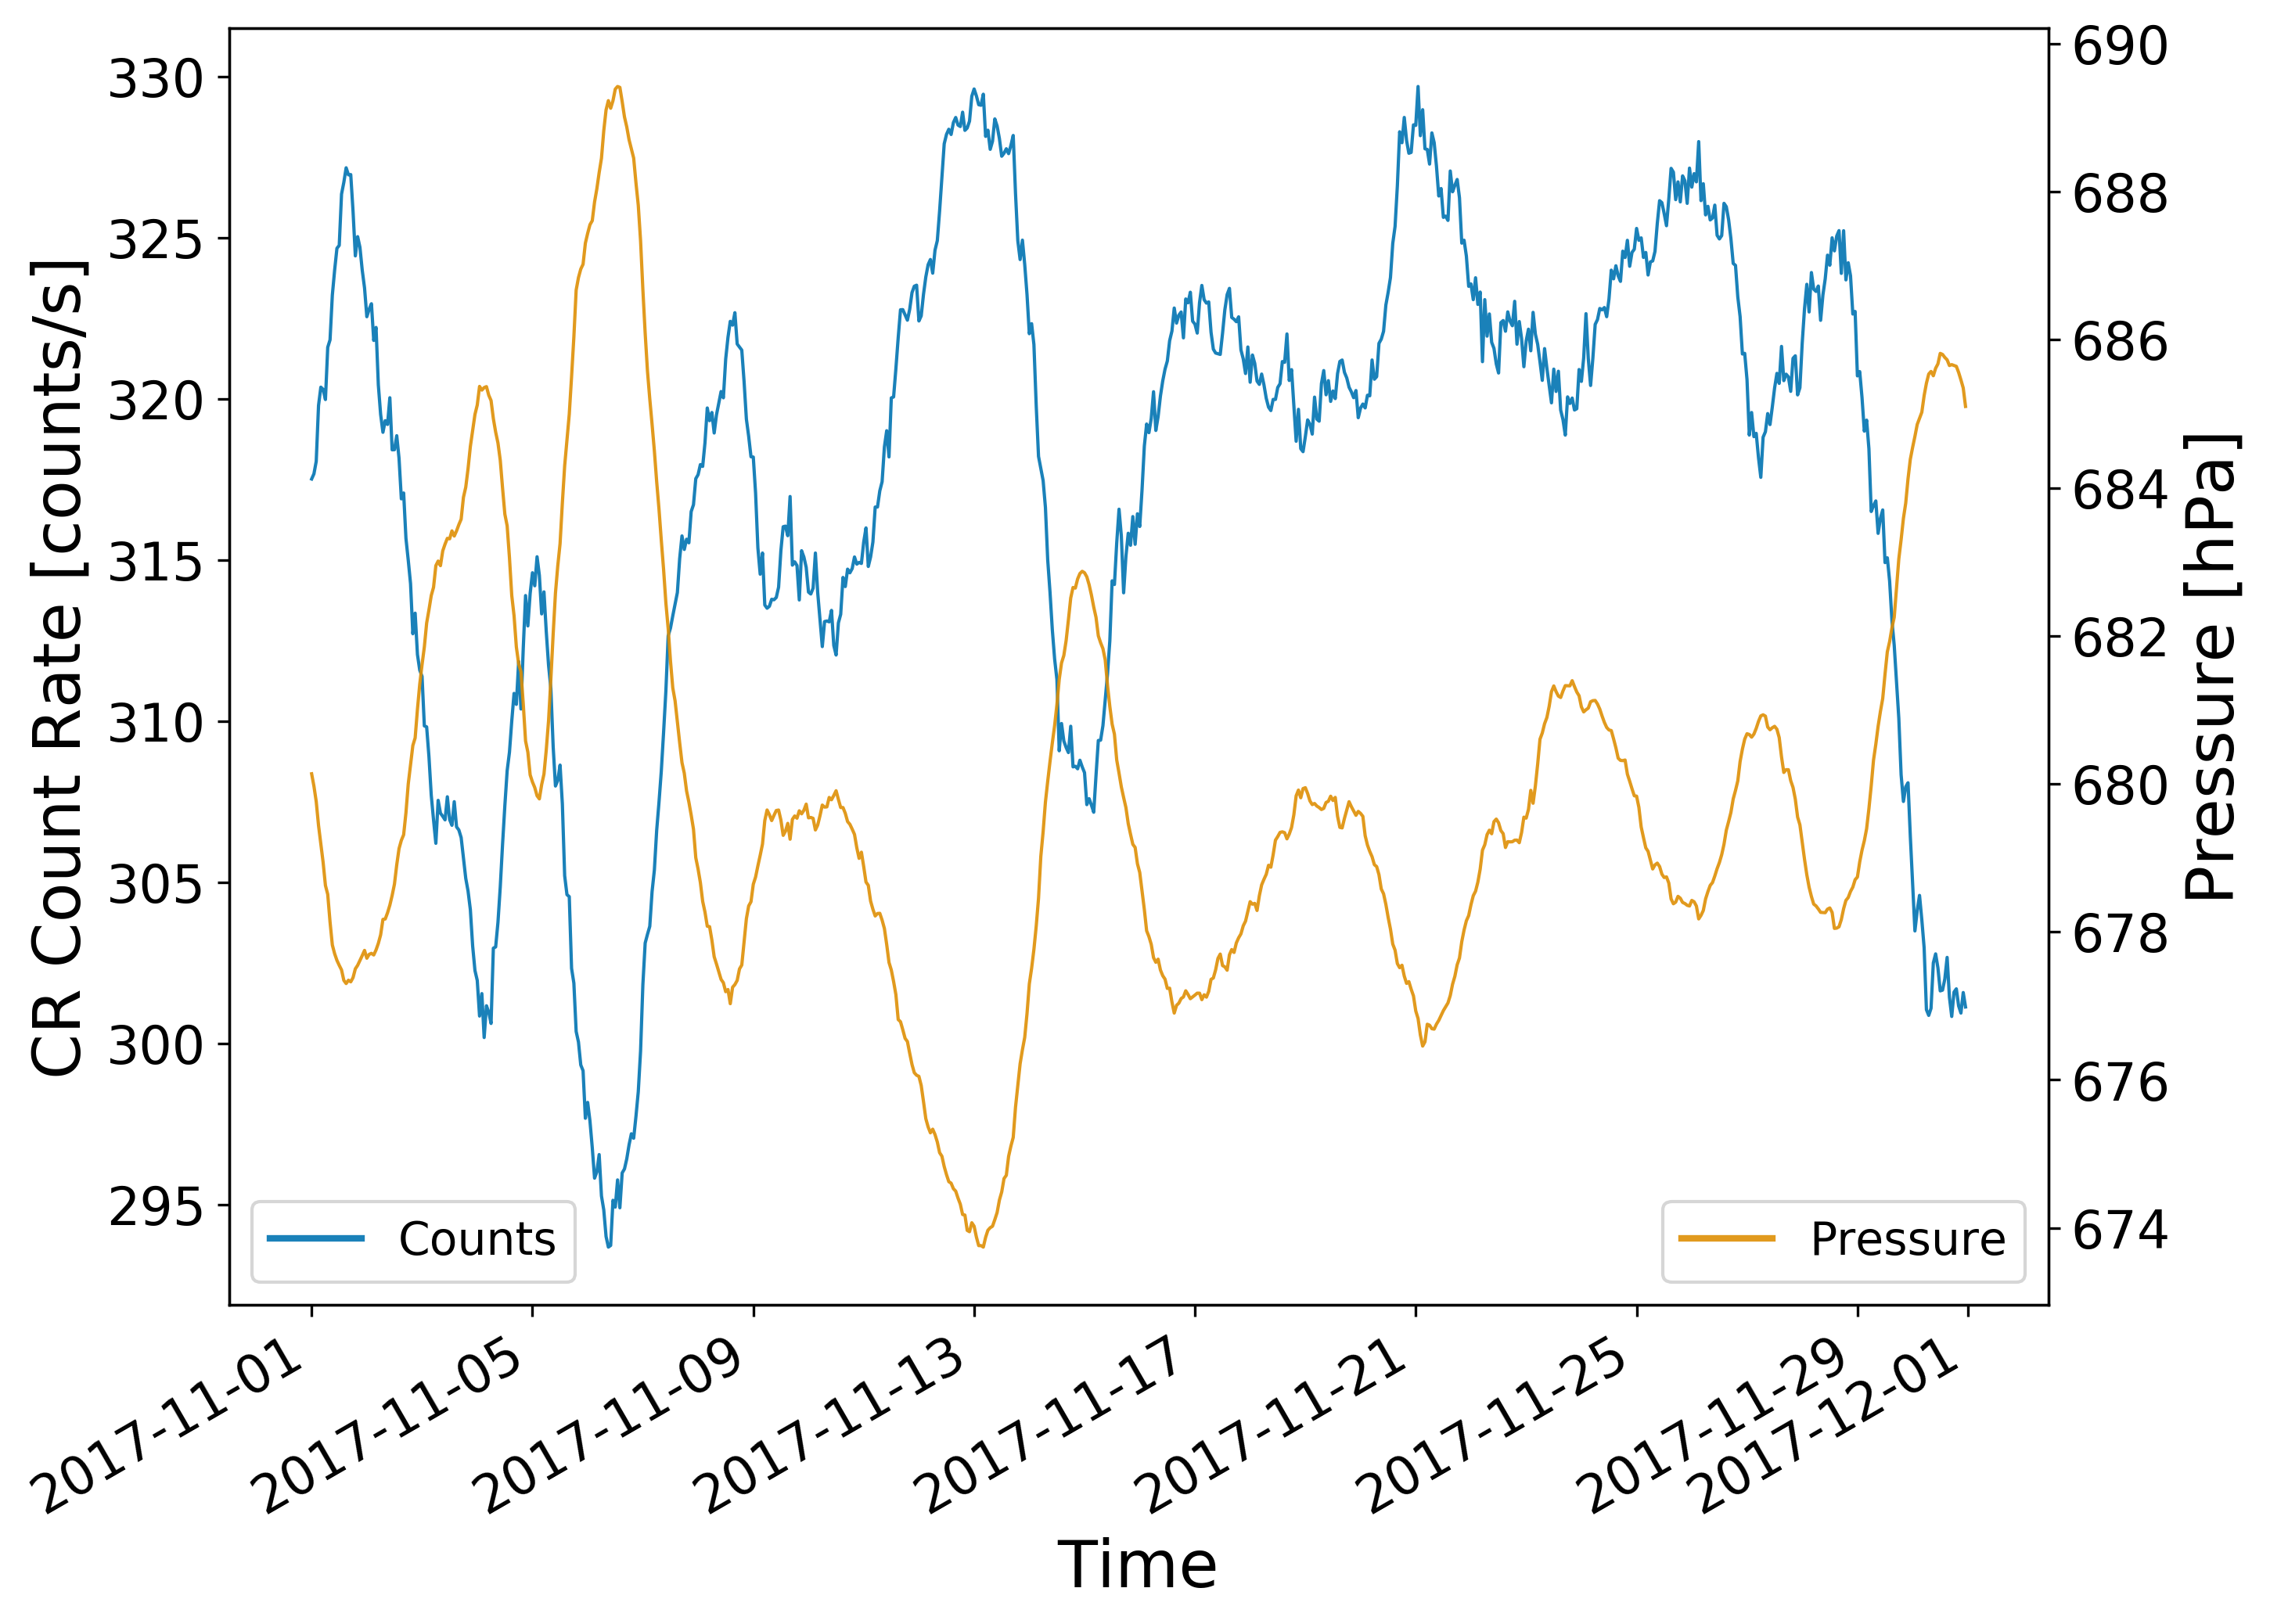
\includegraphics[width=0.48\columnwidth]{SOPO_CRvP.png}
		\label{fig:SOPO_CRvP}}
	%\qquad
	\subfloat[HS 501 (Nikhef)]{
		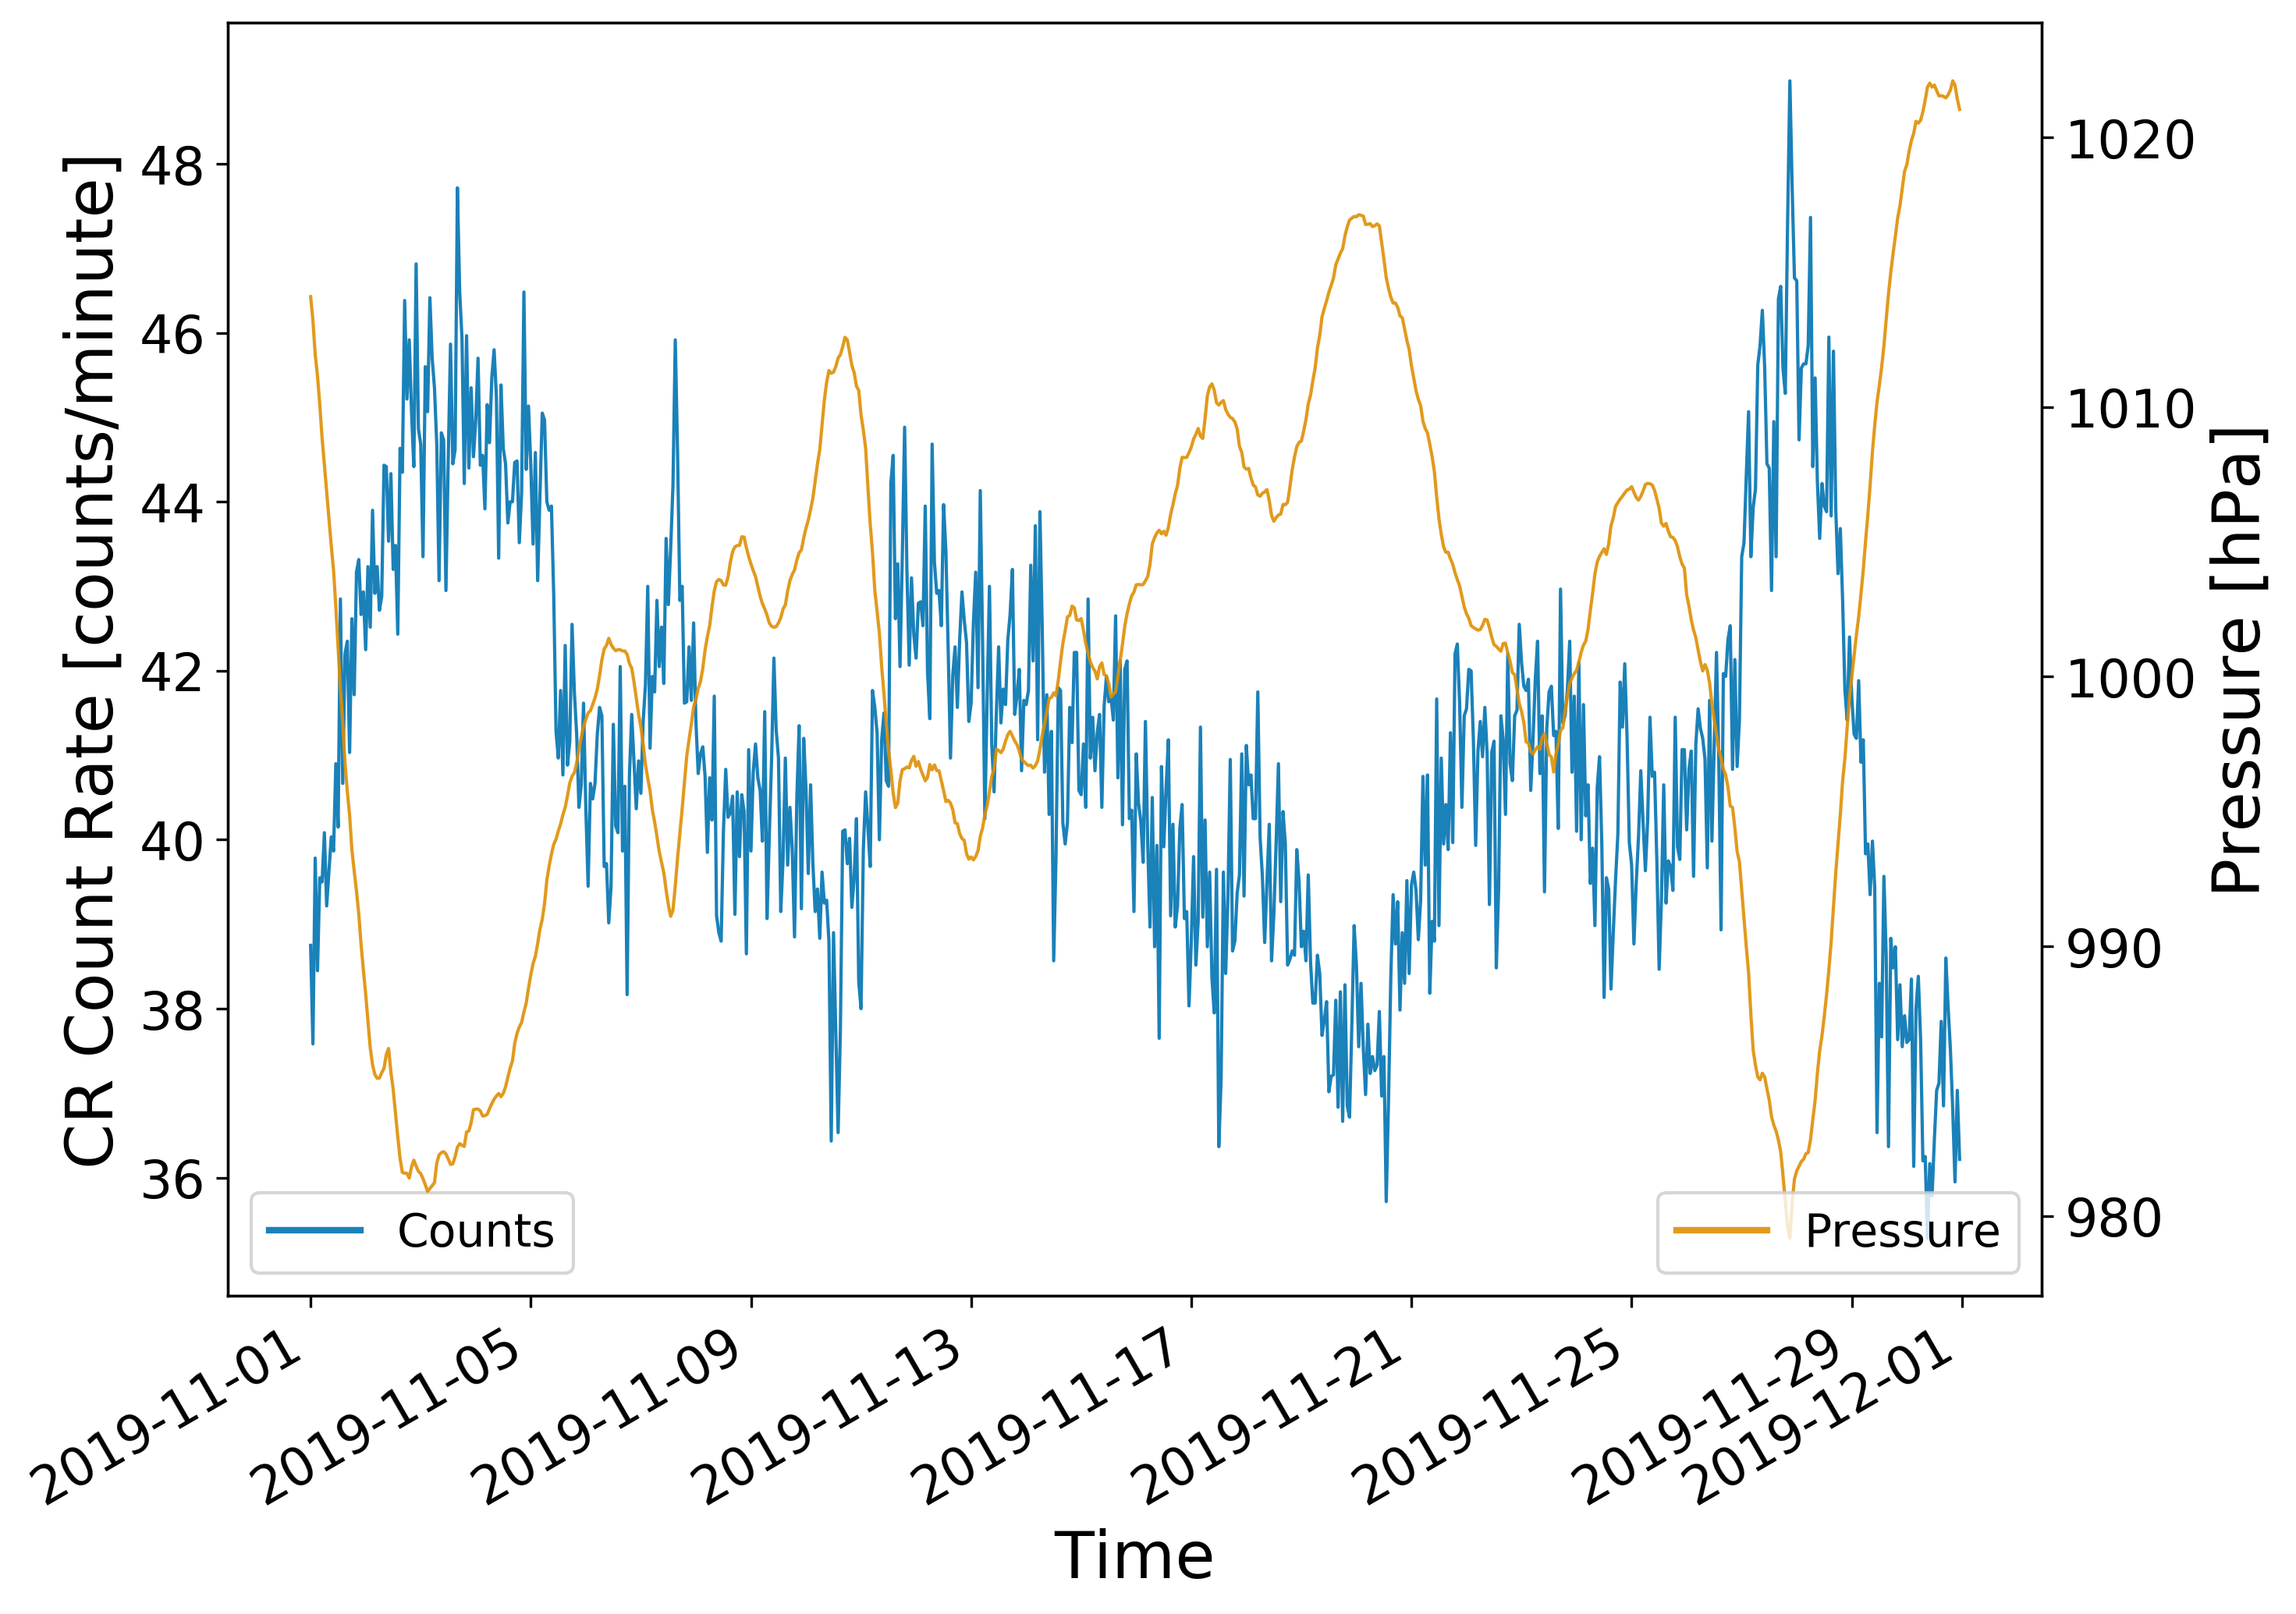
\includegraphics[width=0.48\columnwidth]{501_CRvP.png}
		\label{fig:HS_501_CRvP}} \\
	
	\caption{...}
	\label{fig:CR_V_P}
\end{figure}


The method of correcting for the barometric effect is discussed widely in the literature regarding NMs and is shown to depend on the barometric coefficient. Assuming the cosmic ray flux variation, absent of the atmospheric effects, is reaonably stable, then a simple corrected can be made. The CR variations ($N$) that depend on the local atmospheric pressure are described by equation~(\ref{eq:presscorr1}), where $\Delta N$ is the change in count rate, $\beta$ is the barometric coefficient, and $\Delta P = P - P_0$ is the deviation in pressure from the average ($P_0$) in the given time-period \citep{paschalis_online_2013}:

\begin{equation}
\Delta N = - \beta \, N \, \Delta P
\label{eq:presscorr1}
\end{equation}

Through the integration of equation~(\ref{eq:presscorr1}), the solution shows the dependence of cosmic ray intensity on pressure as given in equation~(\ref{eq:presscorr2}). 

\begin{equation}
N = N_{0} \, e^{-\beta \, \Delta P}
\label{eq:presscorr2}
\end{equation}

Therefore by taking the logarithm of equation~(\ref{eq:presscorr2}), one can obtain the barometric coefficient by fitting the straight line given by equation~(\ref{eq:presscorr3}) to the observed data, where $N_0$ may be assumed as the mean count rate over the given time-period of observations considered.

\begin{equation}
\mathrm{ln} \left( \frac{N}{N_0} \right) = - \beta \, \Delta P
\label{eq:presscorr3}
\end{equation}

A demonstration of the barometric correction method of fitting a straight line to the data described by equation~(\ref{eq:presscorr3}) is shown for both a NM and a HiSPARC station in Figure~\ref{fig:barometric_fit}.

\begin{figure}[ht]
	\centering
	\subfloat[SOPO NM Station]{
		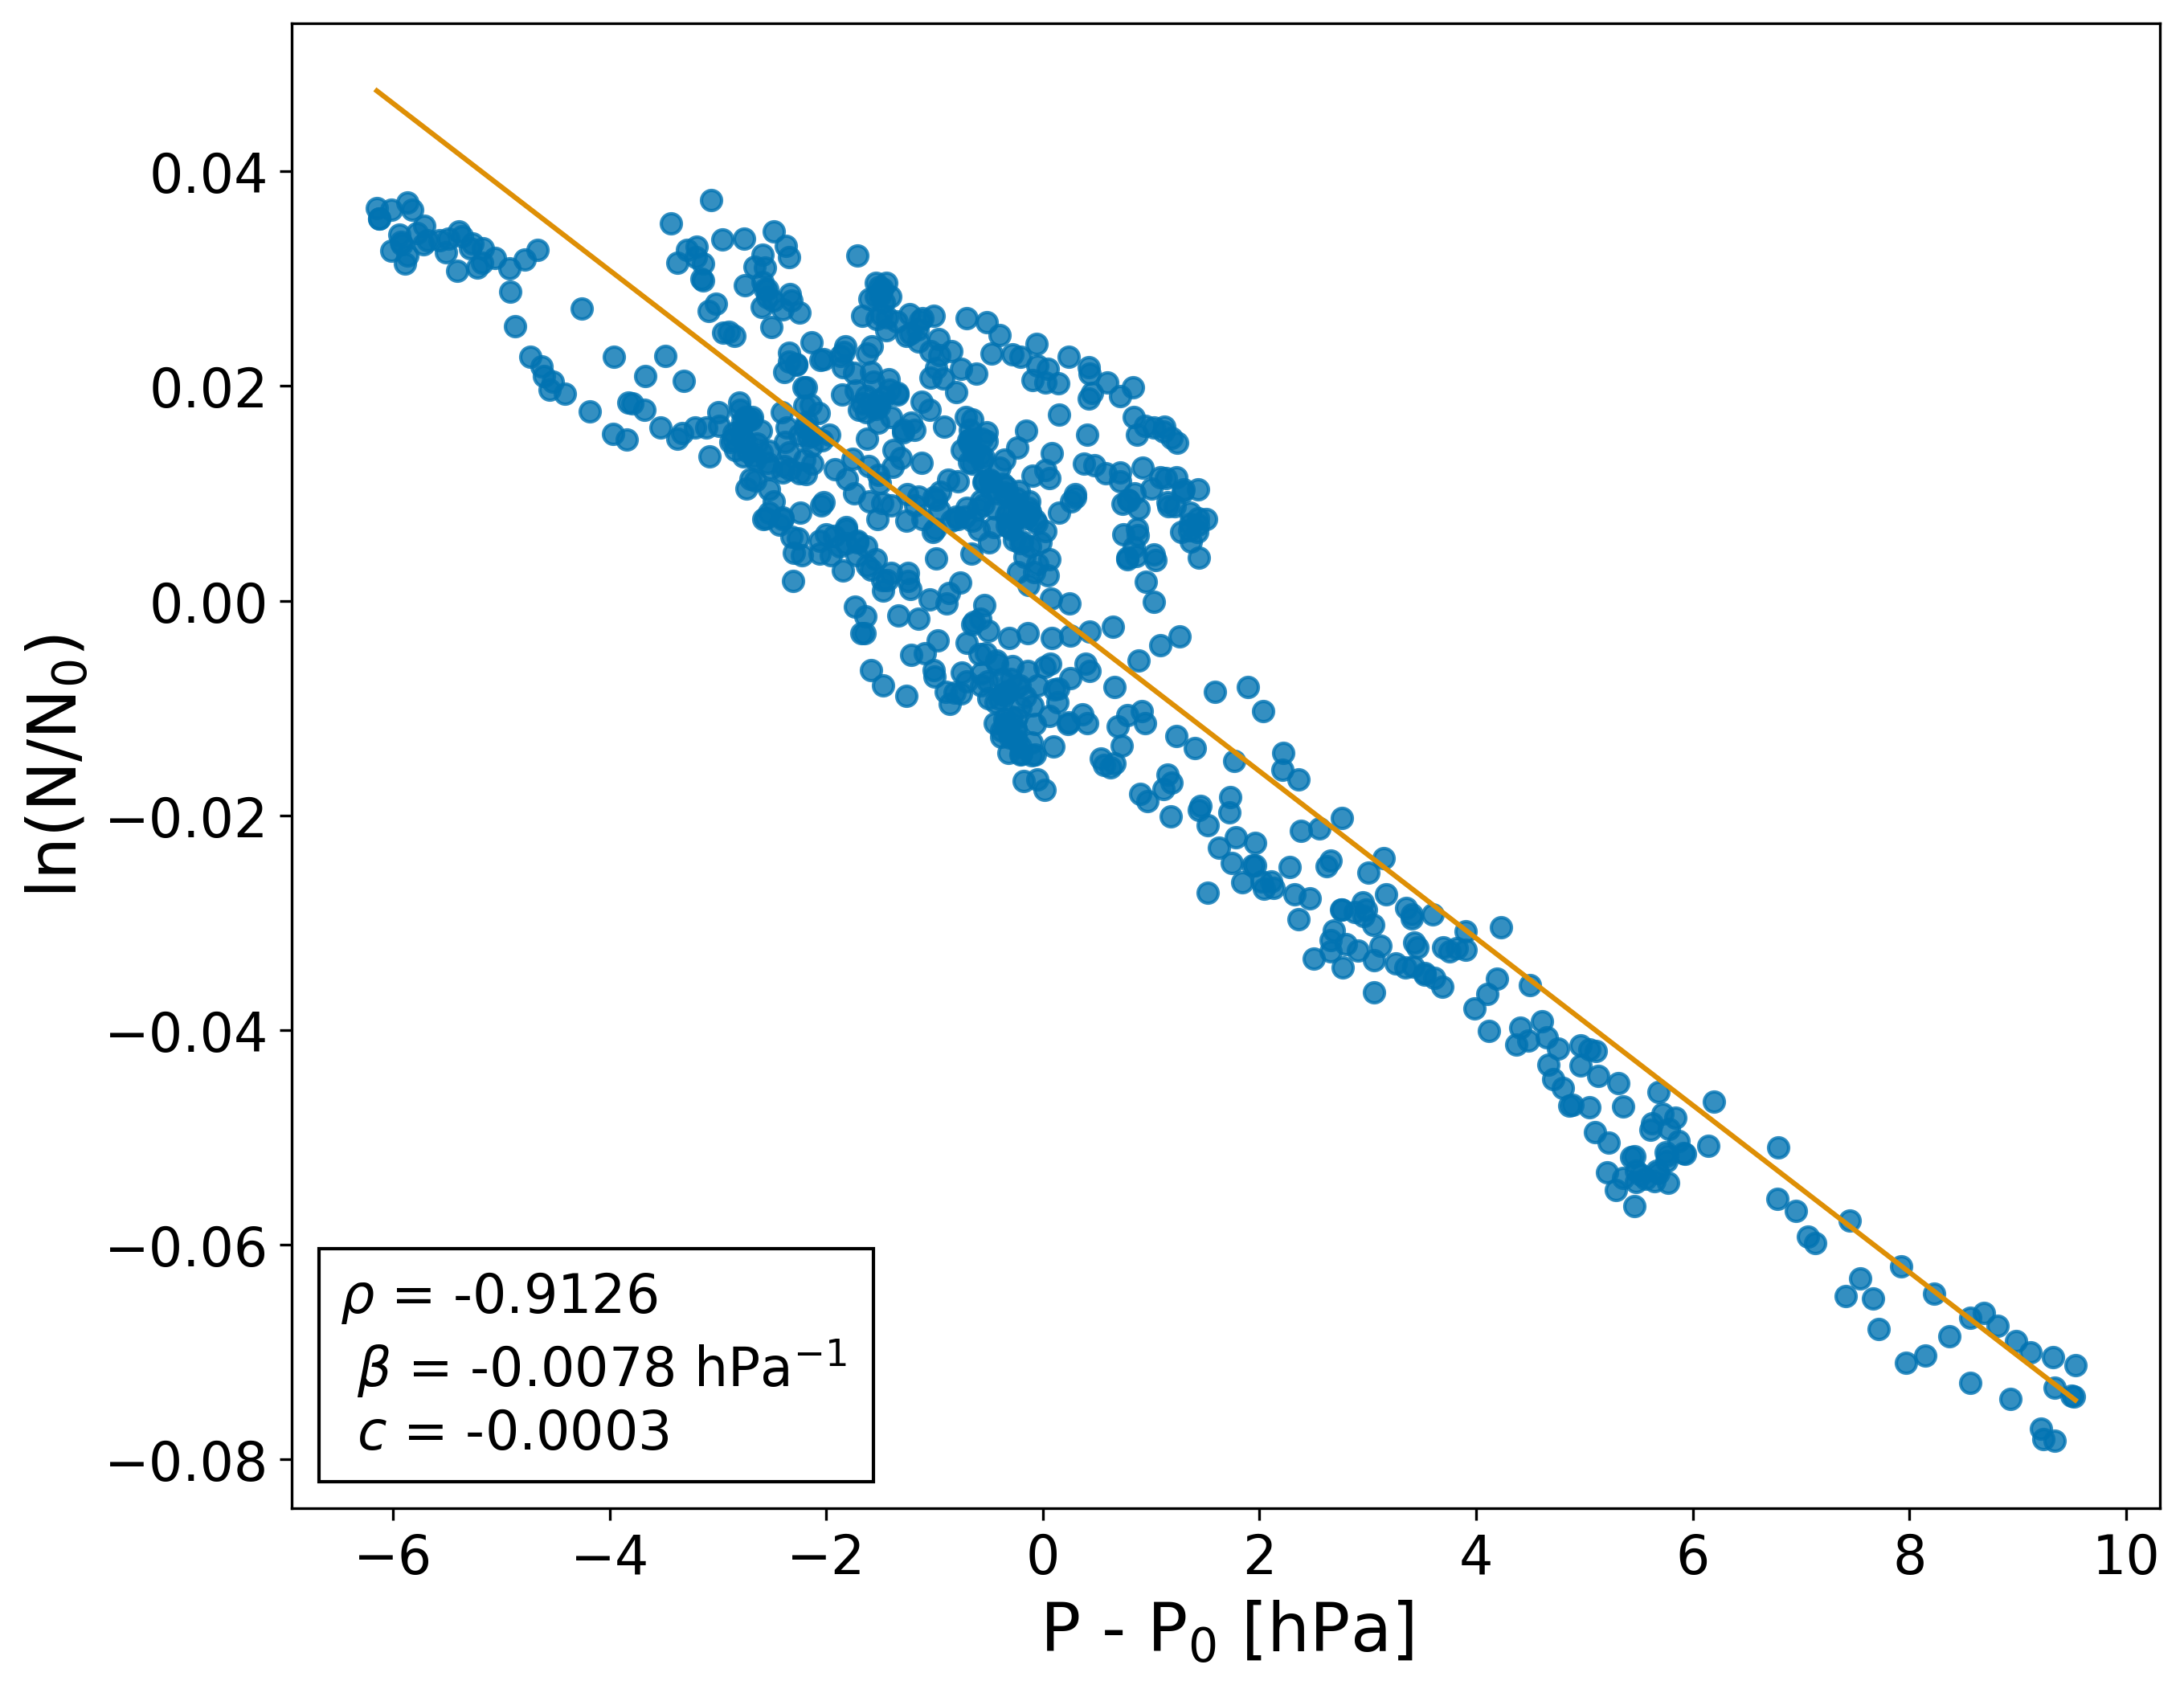
\includegraphics[width=0.48\columnwidth]{SOPO_beta.png}
		\label{fig:SOPO_beta}}
	%\qquad
	\subfloat[HS 501 (Nikhef)]{
		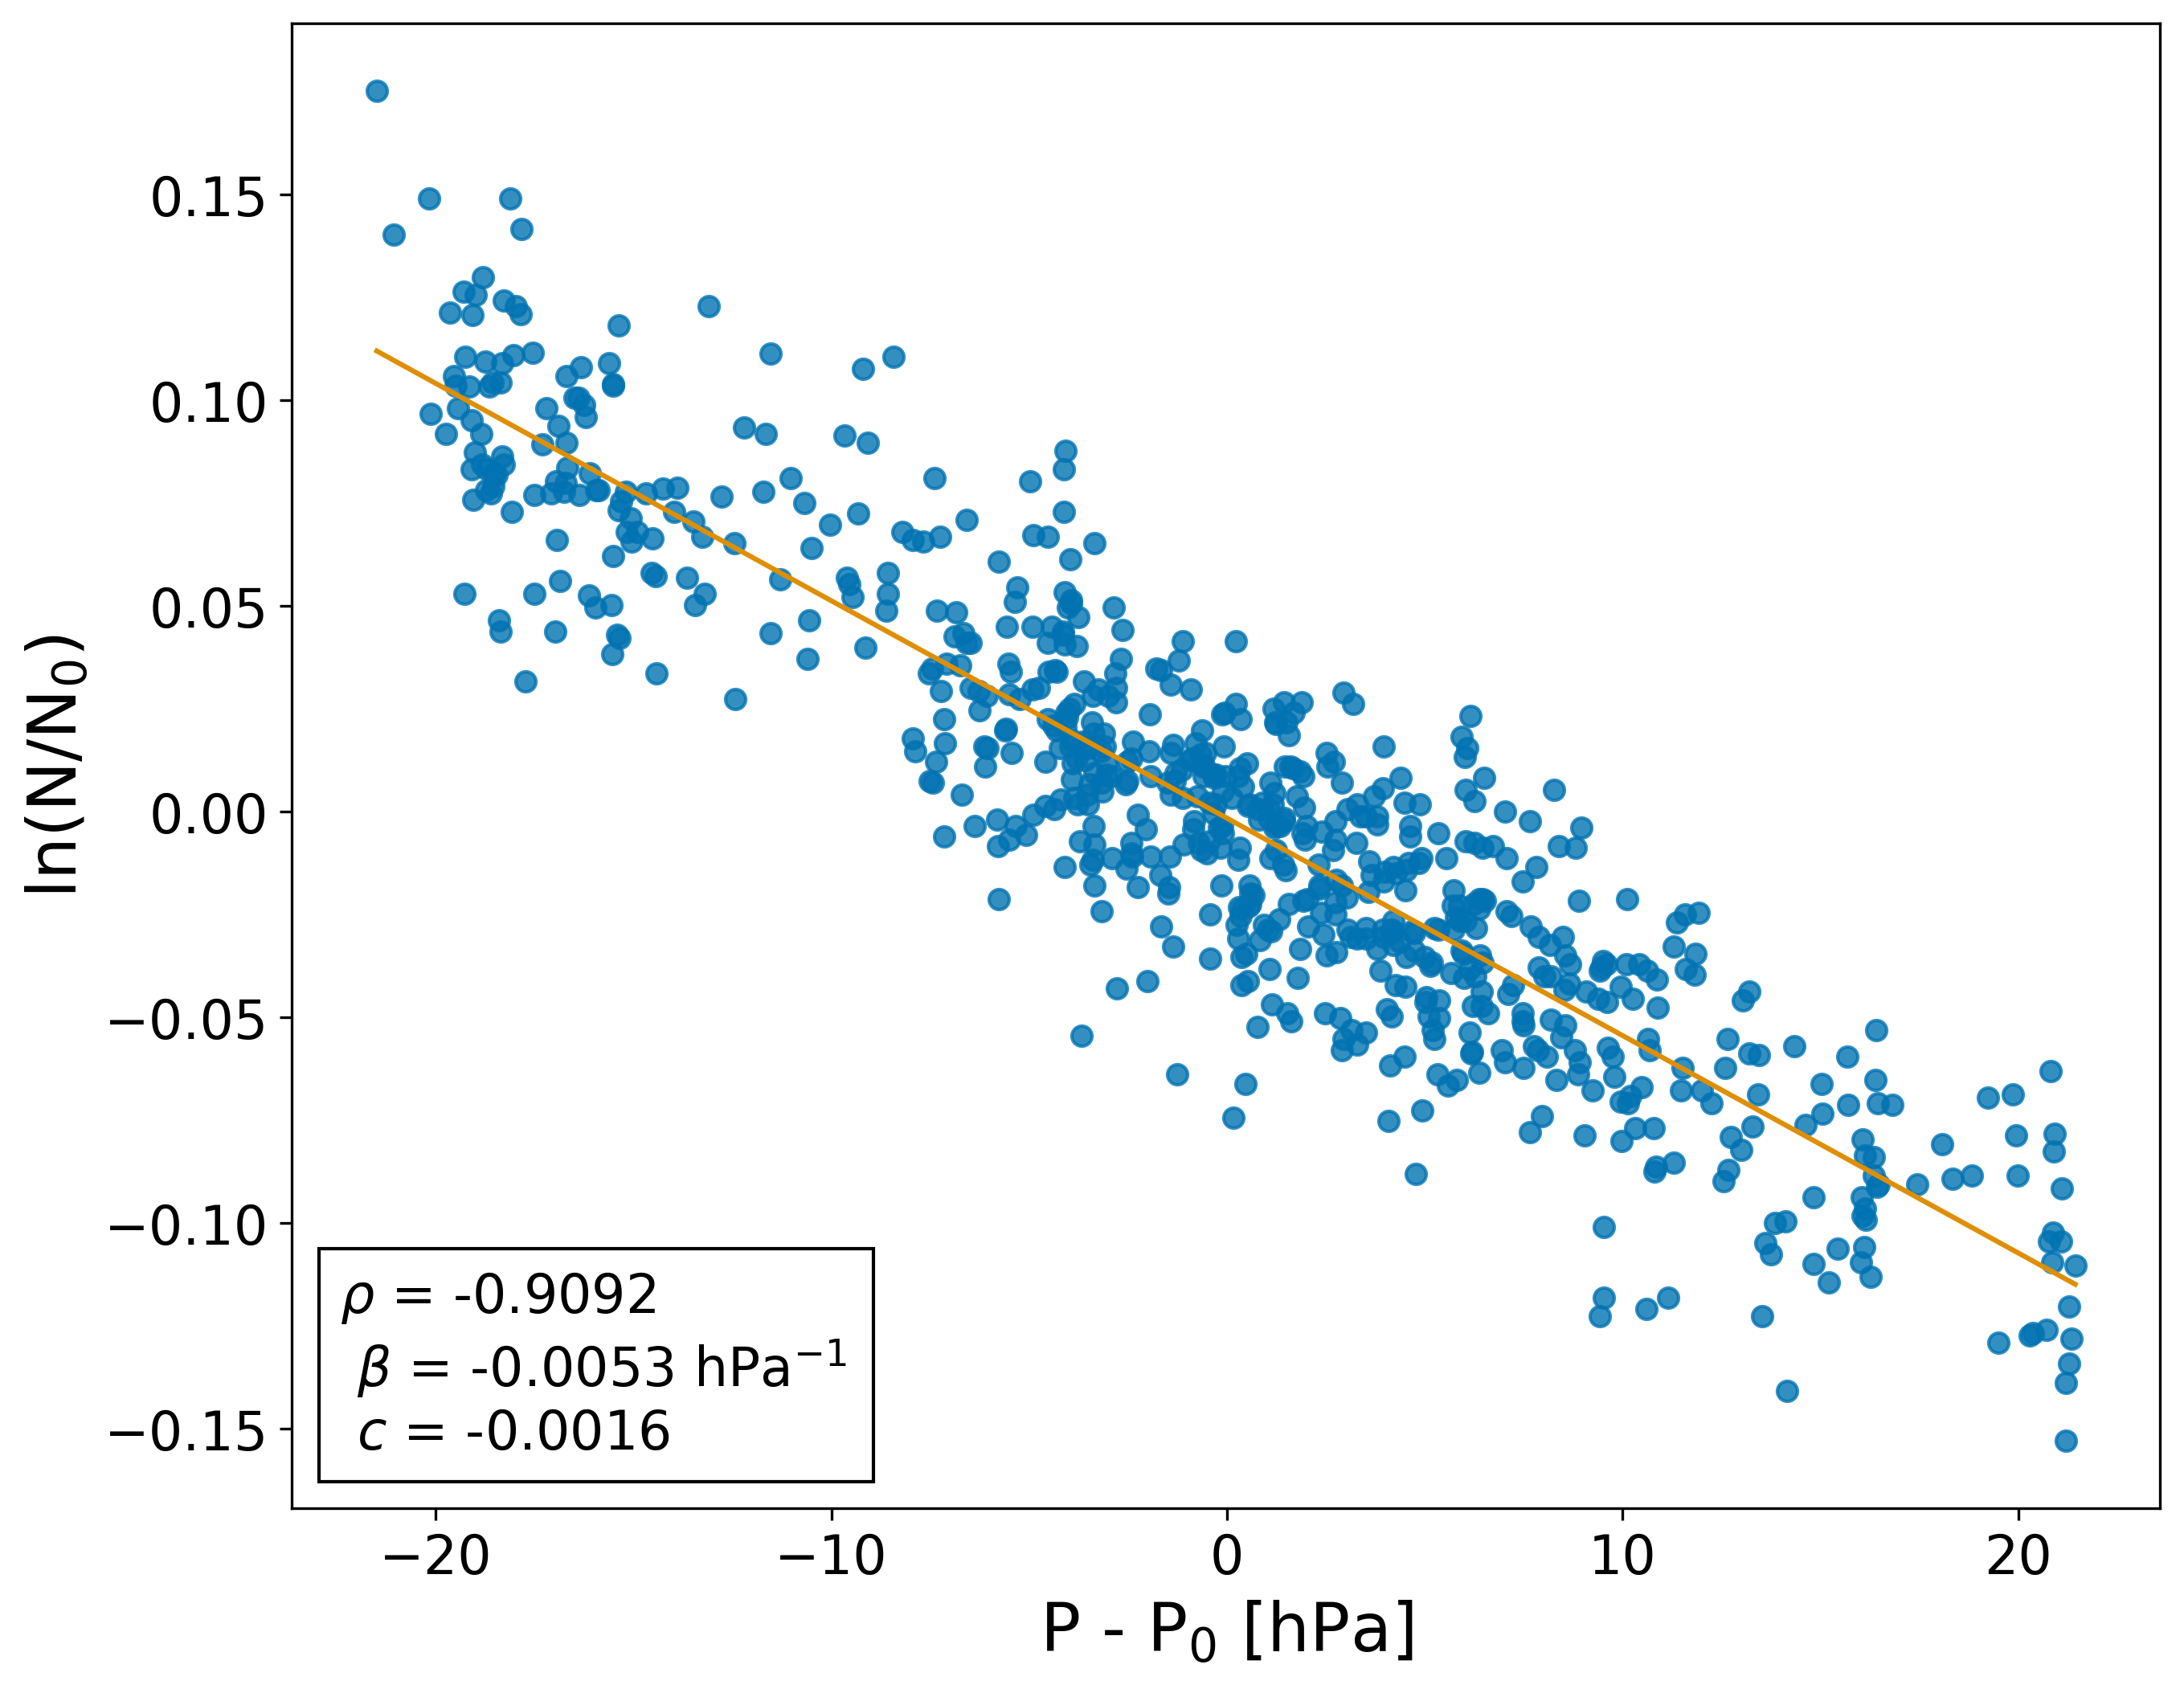
\includegraphics[width=0.48\columnwidth]{501_beta.png}
		\label{fig:HS_501_beta}} \\
	
	\caption{The barometric coefficient calculation: (a) during November 2017 for the South Pole (SOPO) NM station, (b) during November 2019 for HiSPARC station 501 at Nikhef.}
	\label{fig:barometric_fit}
\end{figure}


An online barometric coefficient tool is available which allows user to perform the barometric correction for a given station over a user-defiend epoch (\url{http://cosray.phys.uoa.gr/index.php/data/nm-barometric-coefficient}). Using this tool, it was possible to provide a comparison between the method used in this work to that of the online NM barometric correction tool which is used for the correction of the NMDB stations. This is provided in Figure~\ref{fig:NM_beta_variation} for monthly corrections throughout 2017 for the NM station at the South Pole (SOPO).

\begin{figure}[ht]
	\centering
	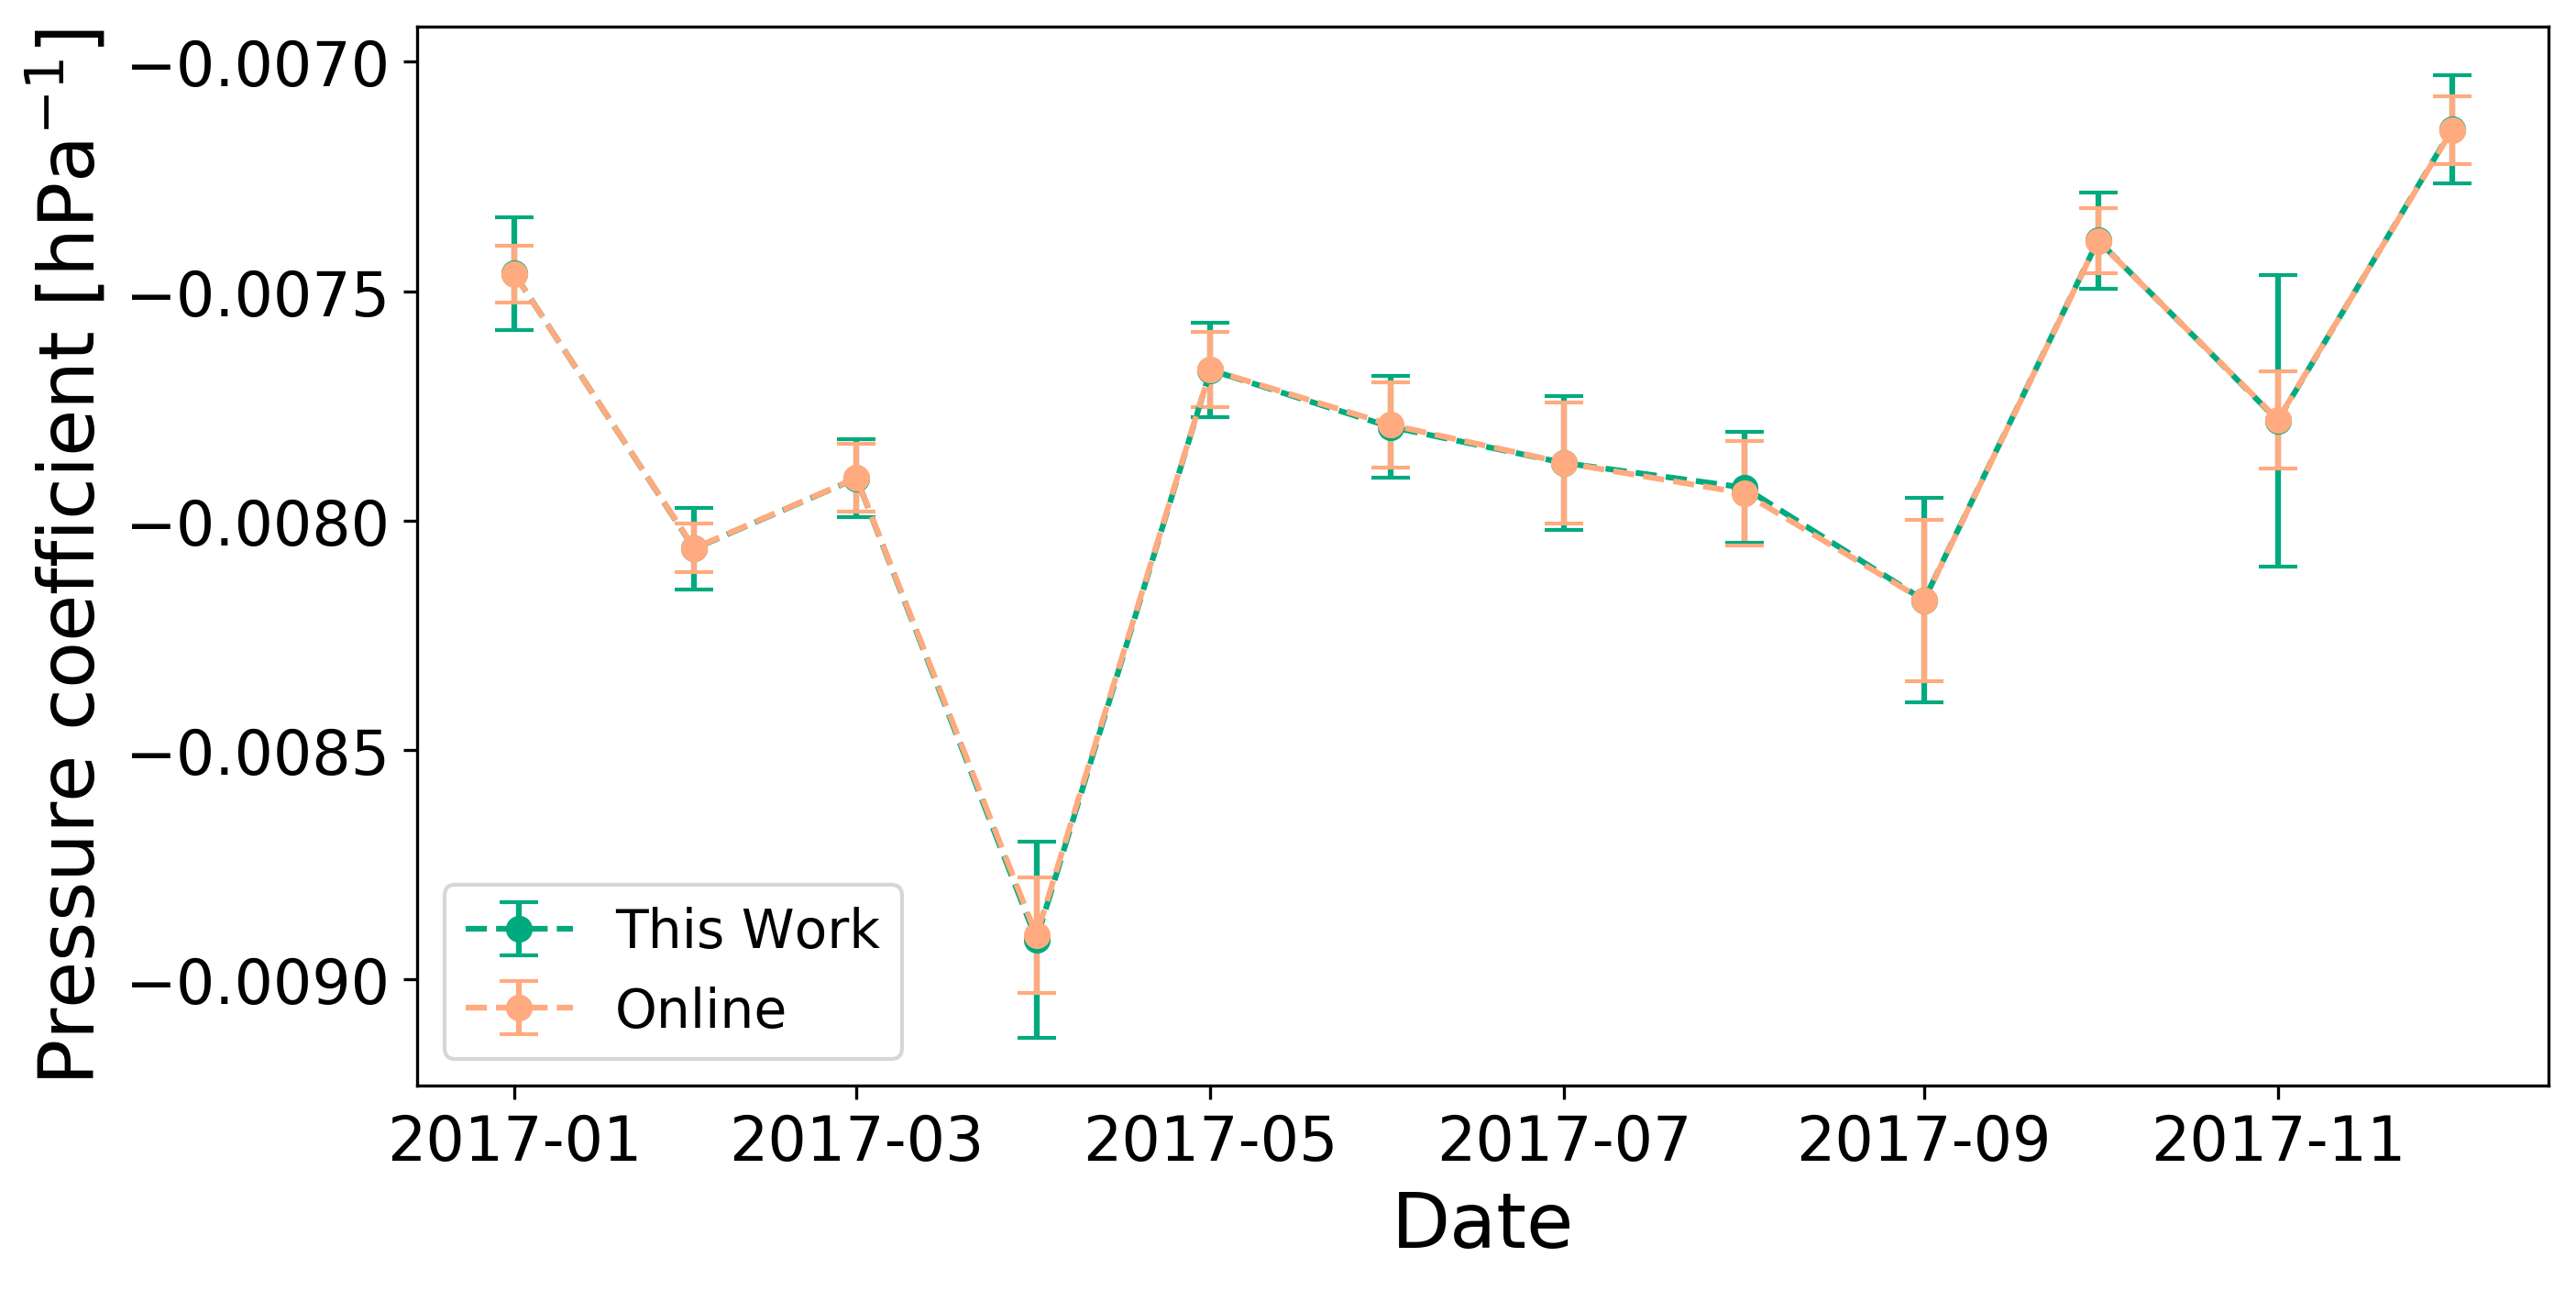
\includegraphics[width=0.65\columnwidth]{SOPO_beta_2017.png}
	\caption{A comparison between the monthly barometric coefficient computed in this work and using the online barometric coefficient tool throughout the year 2017 for the SOPO NM station.}
	\label{fig:NM_beta_variation}
\end{figure}


Figure~\ref{fig:NM_beta_variation} shows a close agreement between the barometric coefficient calculated in this work and those acquired from the online tool for the SOPO NM. This was also true for other stations tested (APTY and ROME), thus providing confidence that the method used in this work was suitable for application on the HiSPARC data. The barometric correction was perfoemed on the stations where sufficient pressure data and count rates exist, and were re-investigated to determine whether the space weather events were observed in the HiSPARC data. These results are provided in Section \ref{sec:HS_obs_Pcorr}.



%%%%%%%%%%%%%%%%%%%%%%%%%%%%%%%%%%%%%%%%%%%%%%%%%%%%%%%%%%%%%%%%%%%%%
\subsection{Temperature Correction}\label{sec:HS_T_corr}

It has been discussed in the literature that the effect of atmospheric temperature on muon intensity has to be treated differently to the pressure effect \citep{berkova_temperature_2011}, as the temperature influences both the creation and disintegration processes for muons, such that there is a positive effect and a negative effect on muon intensity as a consequence of temperature variations \citep{mendoncca_temperature_2016}. 

The positive effect is related to pion decay and its dependence on temperature variation. The higher the temperature, the lower the atmospheric pion absorption, which implies a higher generation rate of muons \citep{mendoncca_temperature_2016}.

The negative effect corresponds to the decrease of muon intensity at ground level as the muon average path length varies with temperature. Due to the heating and the expansion of the atmosphere during summer periods muons are produced higher in the atmosphere; hence the muon propagation path increases meaning more atmosphere for muons to traverse before reaching the ground, and an increased decay probability and ionisation losses \citep{savic_pressure_2015, mendoncca_temperature_2016}.

Due to the difference in decay probability, the negative effects dominate for low energy muons (i.e. those detected by ground-level MDs), and the positive effect dominates for high energy muons (i.e. those detected by underground MDs) \citep{berkova_temperature_2011}; therefore it is expected that the negative effect should dominate for the HiSPARC network. Temperature effects are also observed by NMs; however the effect is less significant than for MDs hence temperature corrections are not widely applied for NMs \citep{mendoncca_temperature_2016}.

This is in contradiction with the observations of diurnal variation with the HiSPARC detector, as one can quite clearly see that the HiSPARC stations register higher count rates during local noon.

Several methods of correcting for the negative temperature effect are summarised by \cite{berkova_temperature_2011} which utilise different measures of atmospheric temperature when performing the temperature correction. \cite{mendoncca_temperature_2016} provides a comparative summary of these methods applied to correct for atmospheric temperature variations observed by GMDN detectors. The methods discussed here however are typically applied over long timescales of years with low temporal resolution rather than to account for short timescale variations with periods of less than a day; hence the suitability of these methods is uncertain.

\cite{mendoncca_temperature_2016} concludes that correcting for temperature using the atmospheric mass weighted temperature is one of the most suitable methods for the GMDN as it allows for the highest correlation between long-term CR variations and temperature. The mass weighted method is an approximation for integrating over the vertical atmospheric temperature as is given in Eq. (\ref{eq:tempcorr}):

\begin{equation}
\left( \frac{\Delta N}{N} \right)_T = \, \bar{\alpha}  \int^{h_0}_{0}  \, \delta \, T(h) \, dh = \sum_{i=0}^{n} \frac{x(h_i) - x(h_{i+1})}{x(h_0)} T(h_i)  = \alpha_{\mathrm{MSS}} \delta T_{\mathrm{MSS}}
\label{eq:tempcorr}
\end{equation}

where $h_0$ is the closest to ground altitude; $\delta T_{\mathrm{MSS}}$ is the deviation of the mass weighted atmospheric temperature; $T(h_i)$ is the temperature in degrees kelvin observed at the altitude $h_i$; $x(h_ i)$ is the atmospheric depth at the altitude $h_i$ which is given by Eq. \ref{eq:atmos_depth}:

\begin{equation}
x(h) = \int^{\infty}_{h}  \, \rho (h) \, dh  \, \rho (h) = \frac{P(h)}{T(h)} \frac{M_{mol}}{R} 
\label{eq:atmos_depth}
\end{equation}

where $P(h)$ is the atmospheric pressure profile as a function of depth; $T(h)$ is the atmospheric temperature; $\rho(h)$ is the air density at a given altitude $h$; $M_{mol}$ is the molar mass of air; $R$ is the universal gas constant.

The temperature correction is therefore used in a formalism the same as Eq. (\ref{eq:presscorr3}), replacing replacing $\beta$ for $\alpha$ and $\Delta P$ for $\Delta T$.

In addition it is discussed by \cite{berkova_temperature_2011} and \cite{mendoncca_temperature_2016} that the effective generation level temperature is a suitable assumption for this purpose. This method is based on the assumption that muons are mostly generated at a certain isobaric level, taken as 100 mbar, and therefore the temperature at 100 mbar in the atmospheric pressure profile is used, $T_{\mathrm{100 \, mbar}}$.

As discussed above, \cite{mendoncca_temperature_2016} provide this as a method for correcting for the long-term variation in atmospheric temperature which varies seasonally rather than to correct for diurnal variations; therefore it is unsure how relevant this method of atmospheric temperature correction will be to the diurnal variations observed in the HiSPARC data.



 

%%%%%%%%%%%%%%%%%%%%%%%%%%%%%%%%%%%%%%%%%%%%%%%%%%%%%%%%%%%%%%%%%%%%%
%%%%%%%%%%%%%%%%%%%%%%%%%%%%%%%%%%%%%%%%%%%%%%%%%%%%%%%%%%%%%%%%%%%%%
\section{HiSPARC Observations After Pressure Corrections}\label{sec:HS_obs_Pcorr}


%%%%%%%%%%%%%%%%%%%%%%%%%%%%%%%%%%%%%%%%%%%%%%%%%%%%%%%%%%%%%%%%%%%%%
\subsection{Pressure Corrected Observations of Ground Level Enhancements}


\begin{figure}[ht]
	\centering
	\subfloat[...]{
		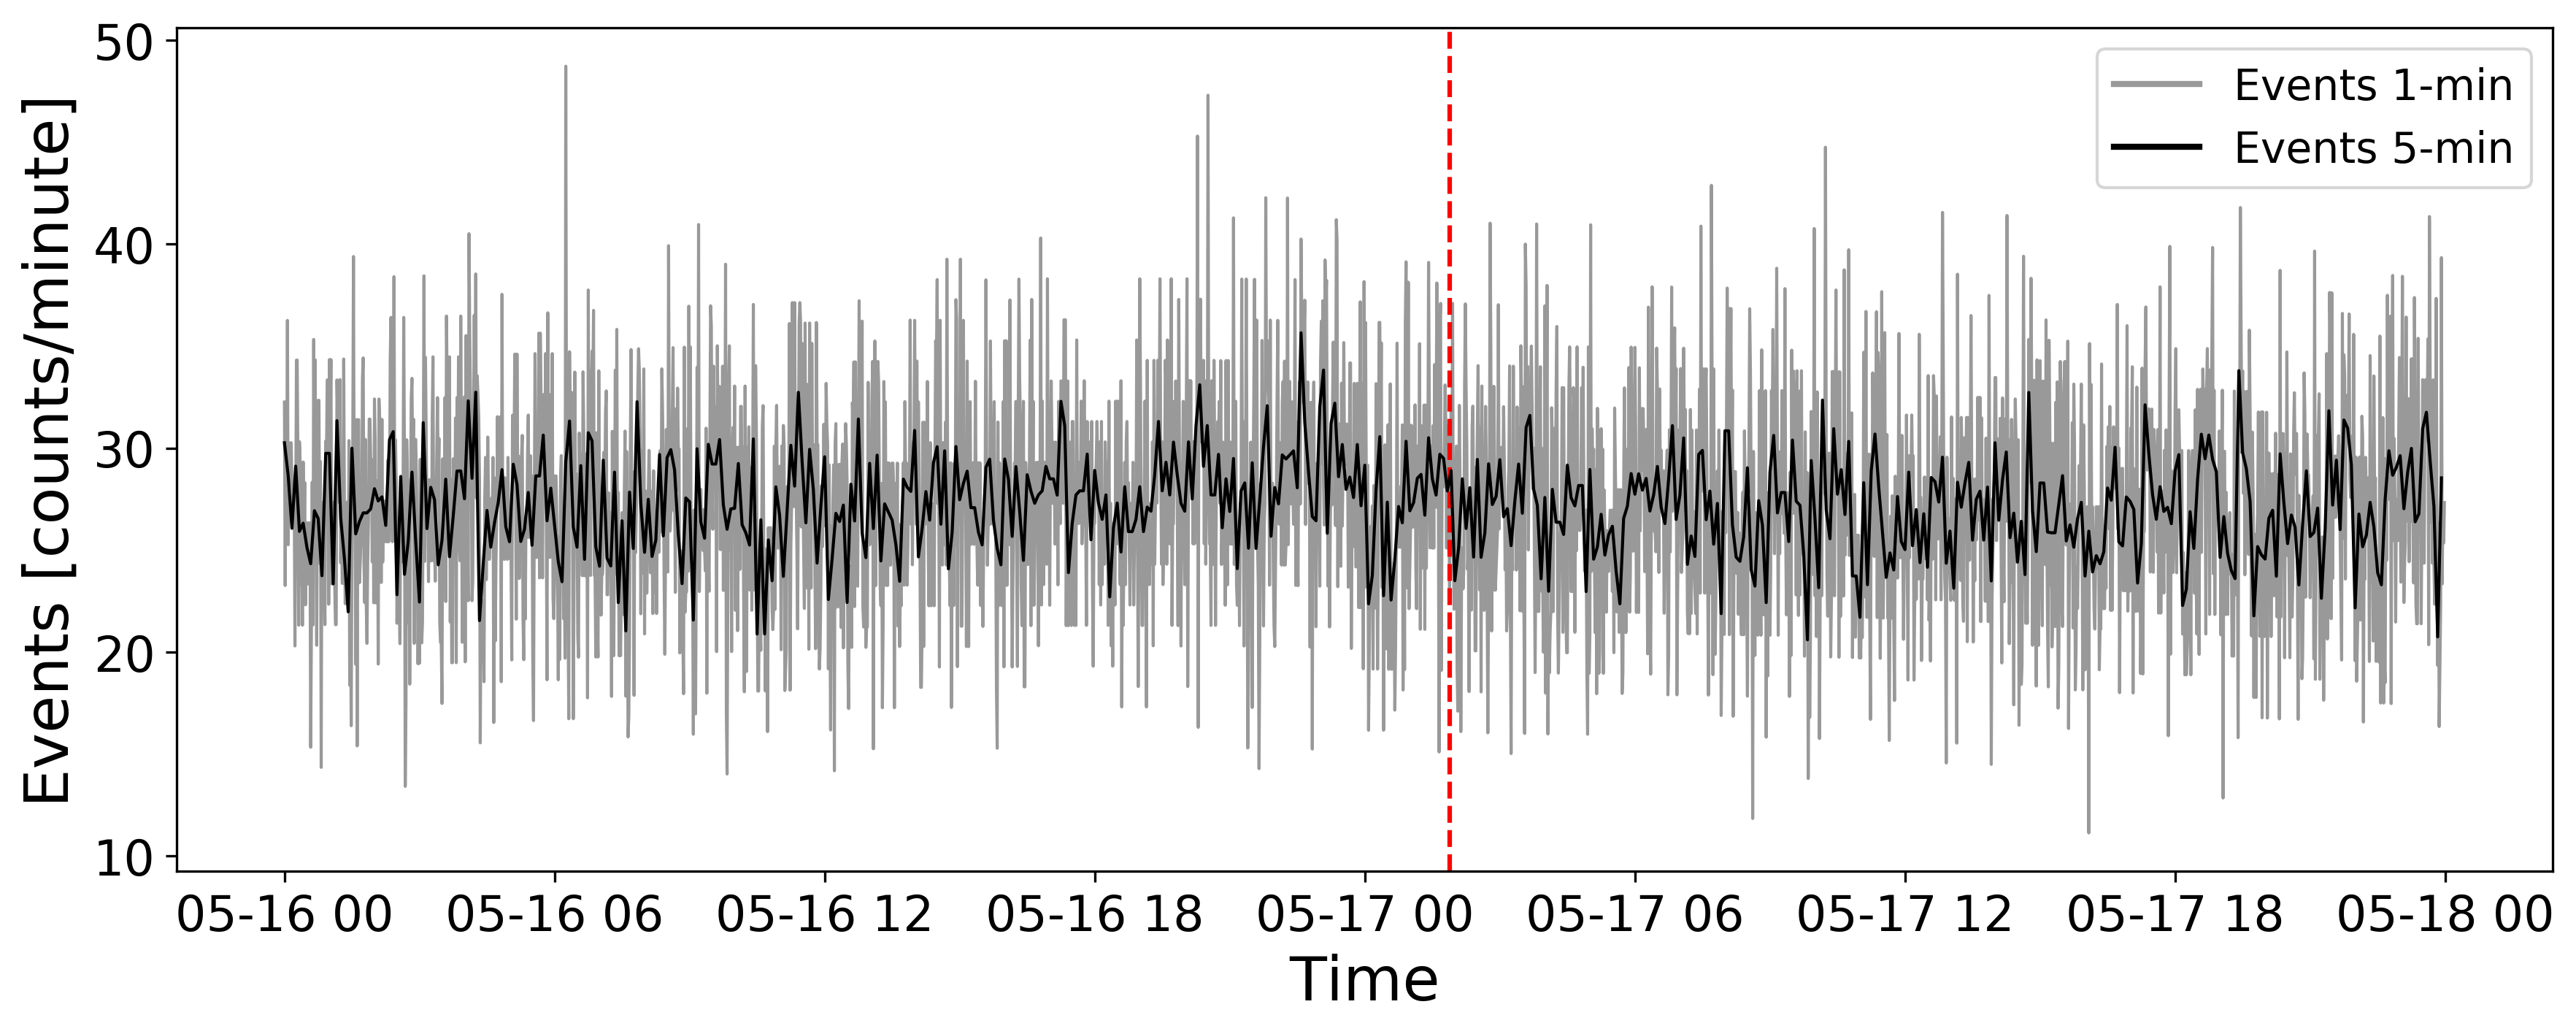
\includegraphics[width=0.48\columnwidth]{GLE71_3001_Pcorr.png}
		\label{fig:GLE71_3001_Pcorr}}
	%\qquad
	\subfloat[...]{
		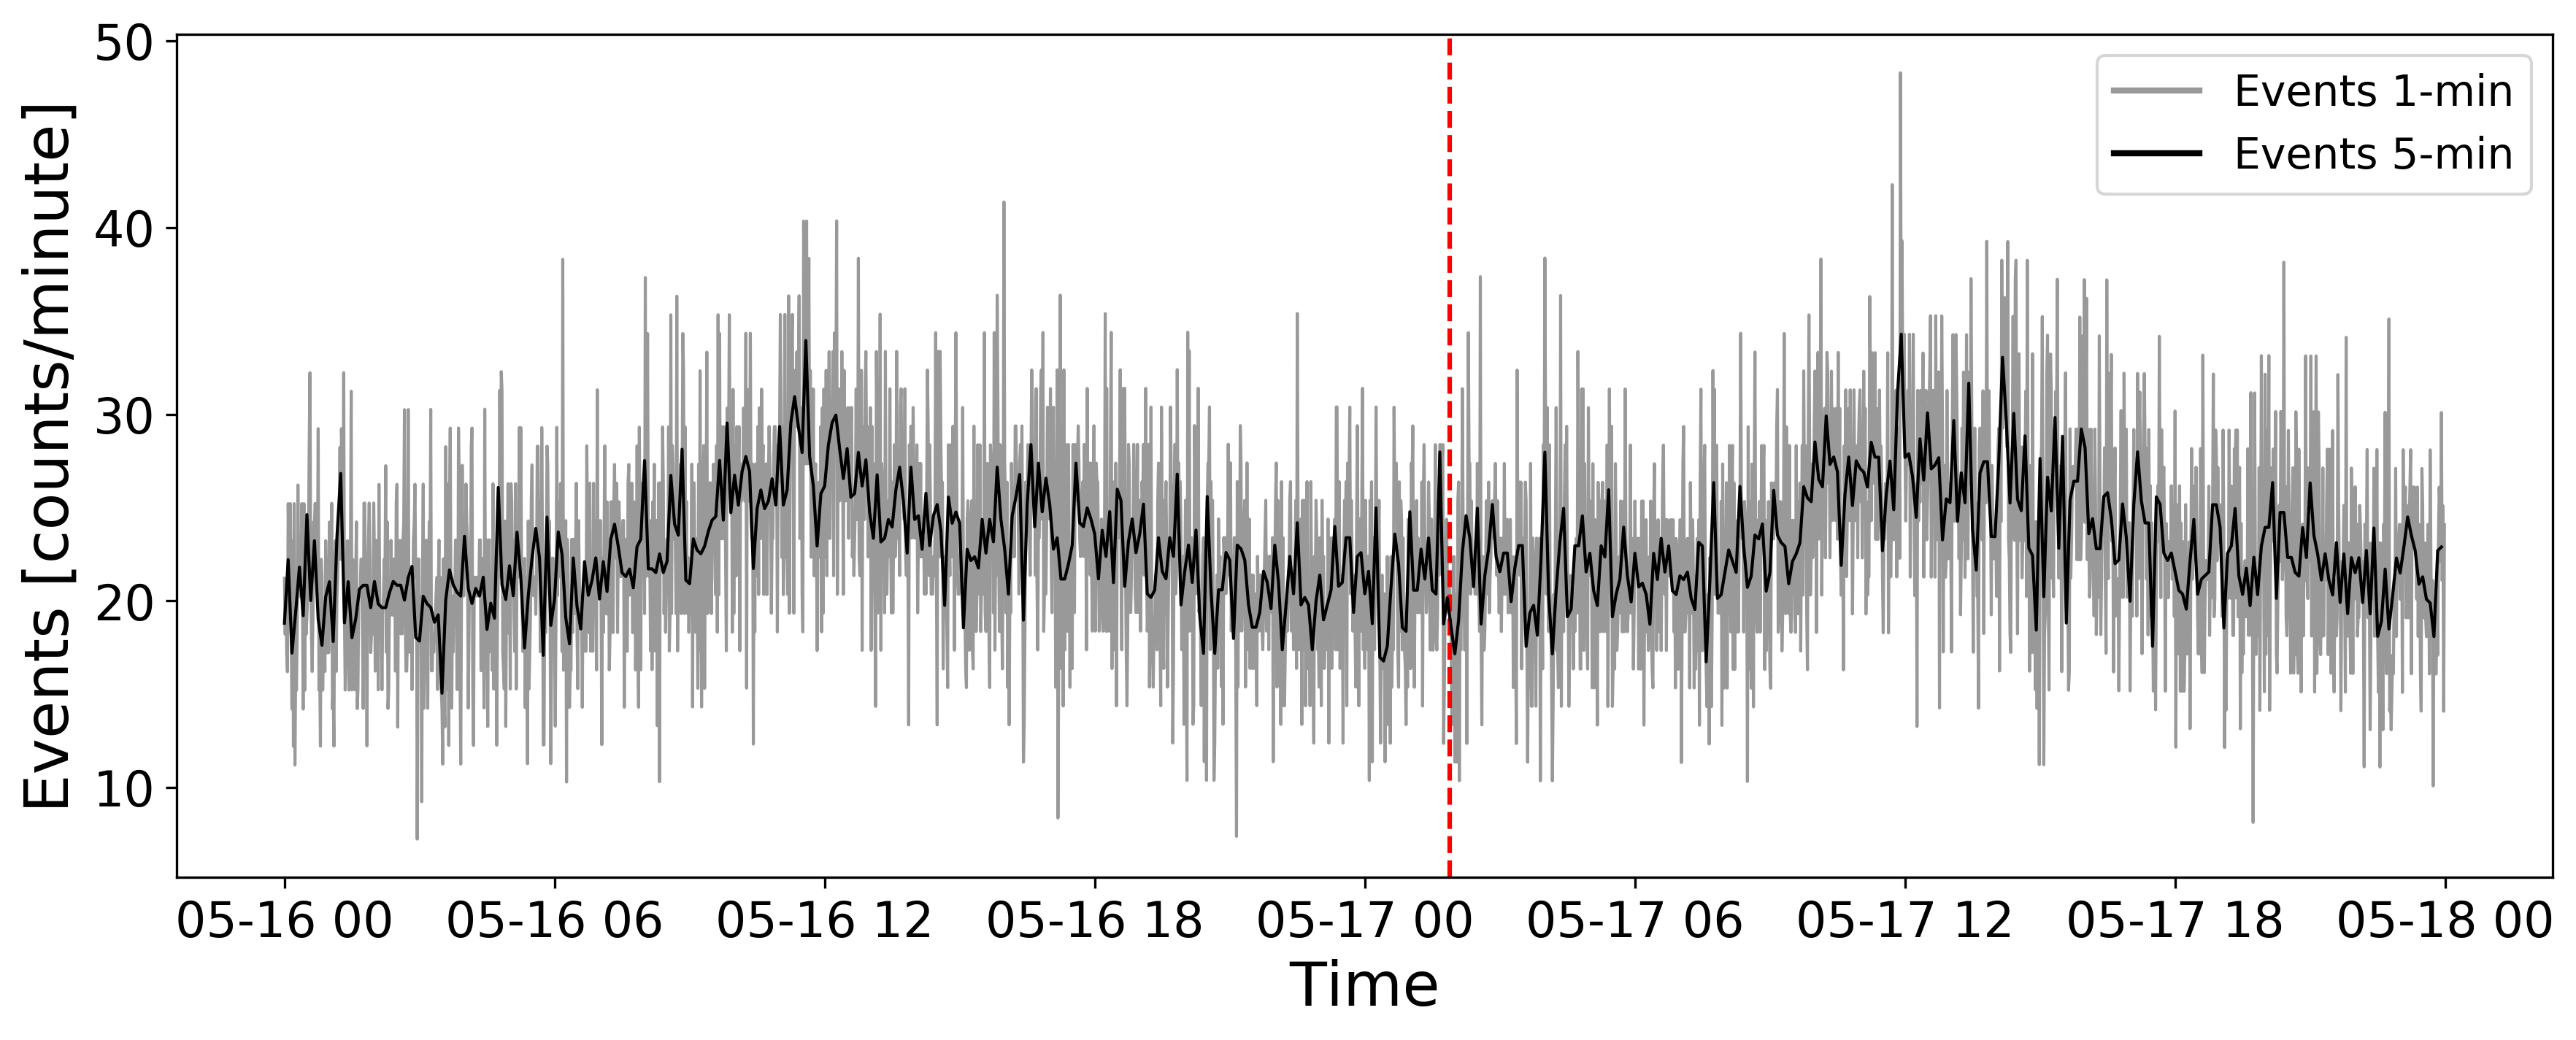
\includegraphics[width=0.48\columnwidth]{GLE71_8001_Pcorr.png}
		\label{fig:GLE71_8001_Pcorr}} \\
	
	
	\caption{Pressure corrected HiSPARC data for 2 stations around the epoch of GLE 71. The top panel of each subplot shows the minute-averaged trigger events between detectors within the station, while the bottom panel shows the mean-shifted, minute-averaged counts by each individual detector in the station. The vertical red, dashed line depicts the approximate onset time of the GLE.}
	\label{fig:GLE_71_Pcorr}
\end{figure}


\begin{figure}[ht]
	\centering
	\subfloat[HS 501 (Nikhef)]{
		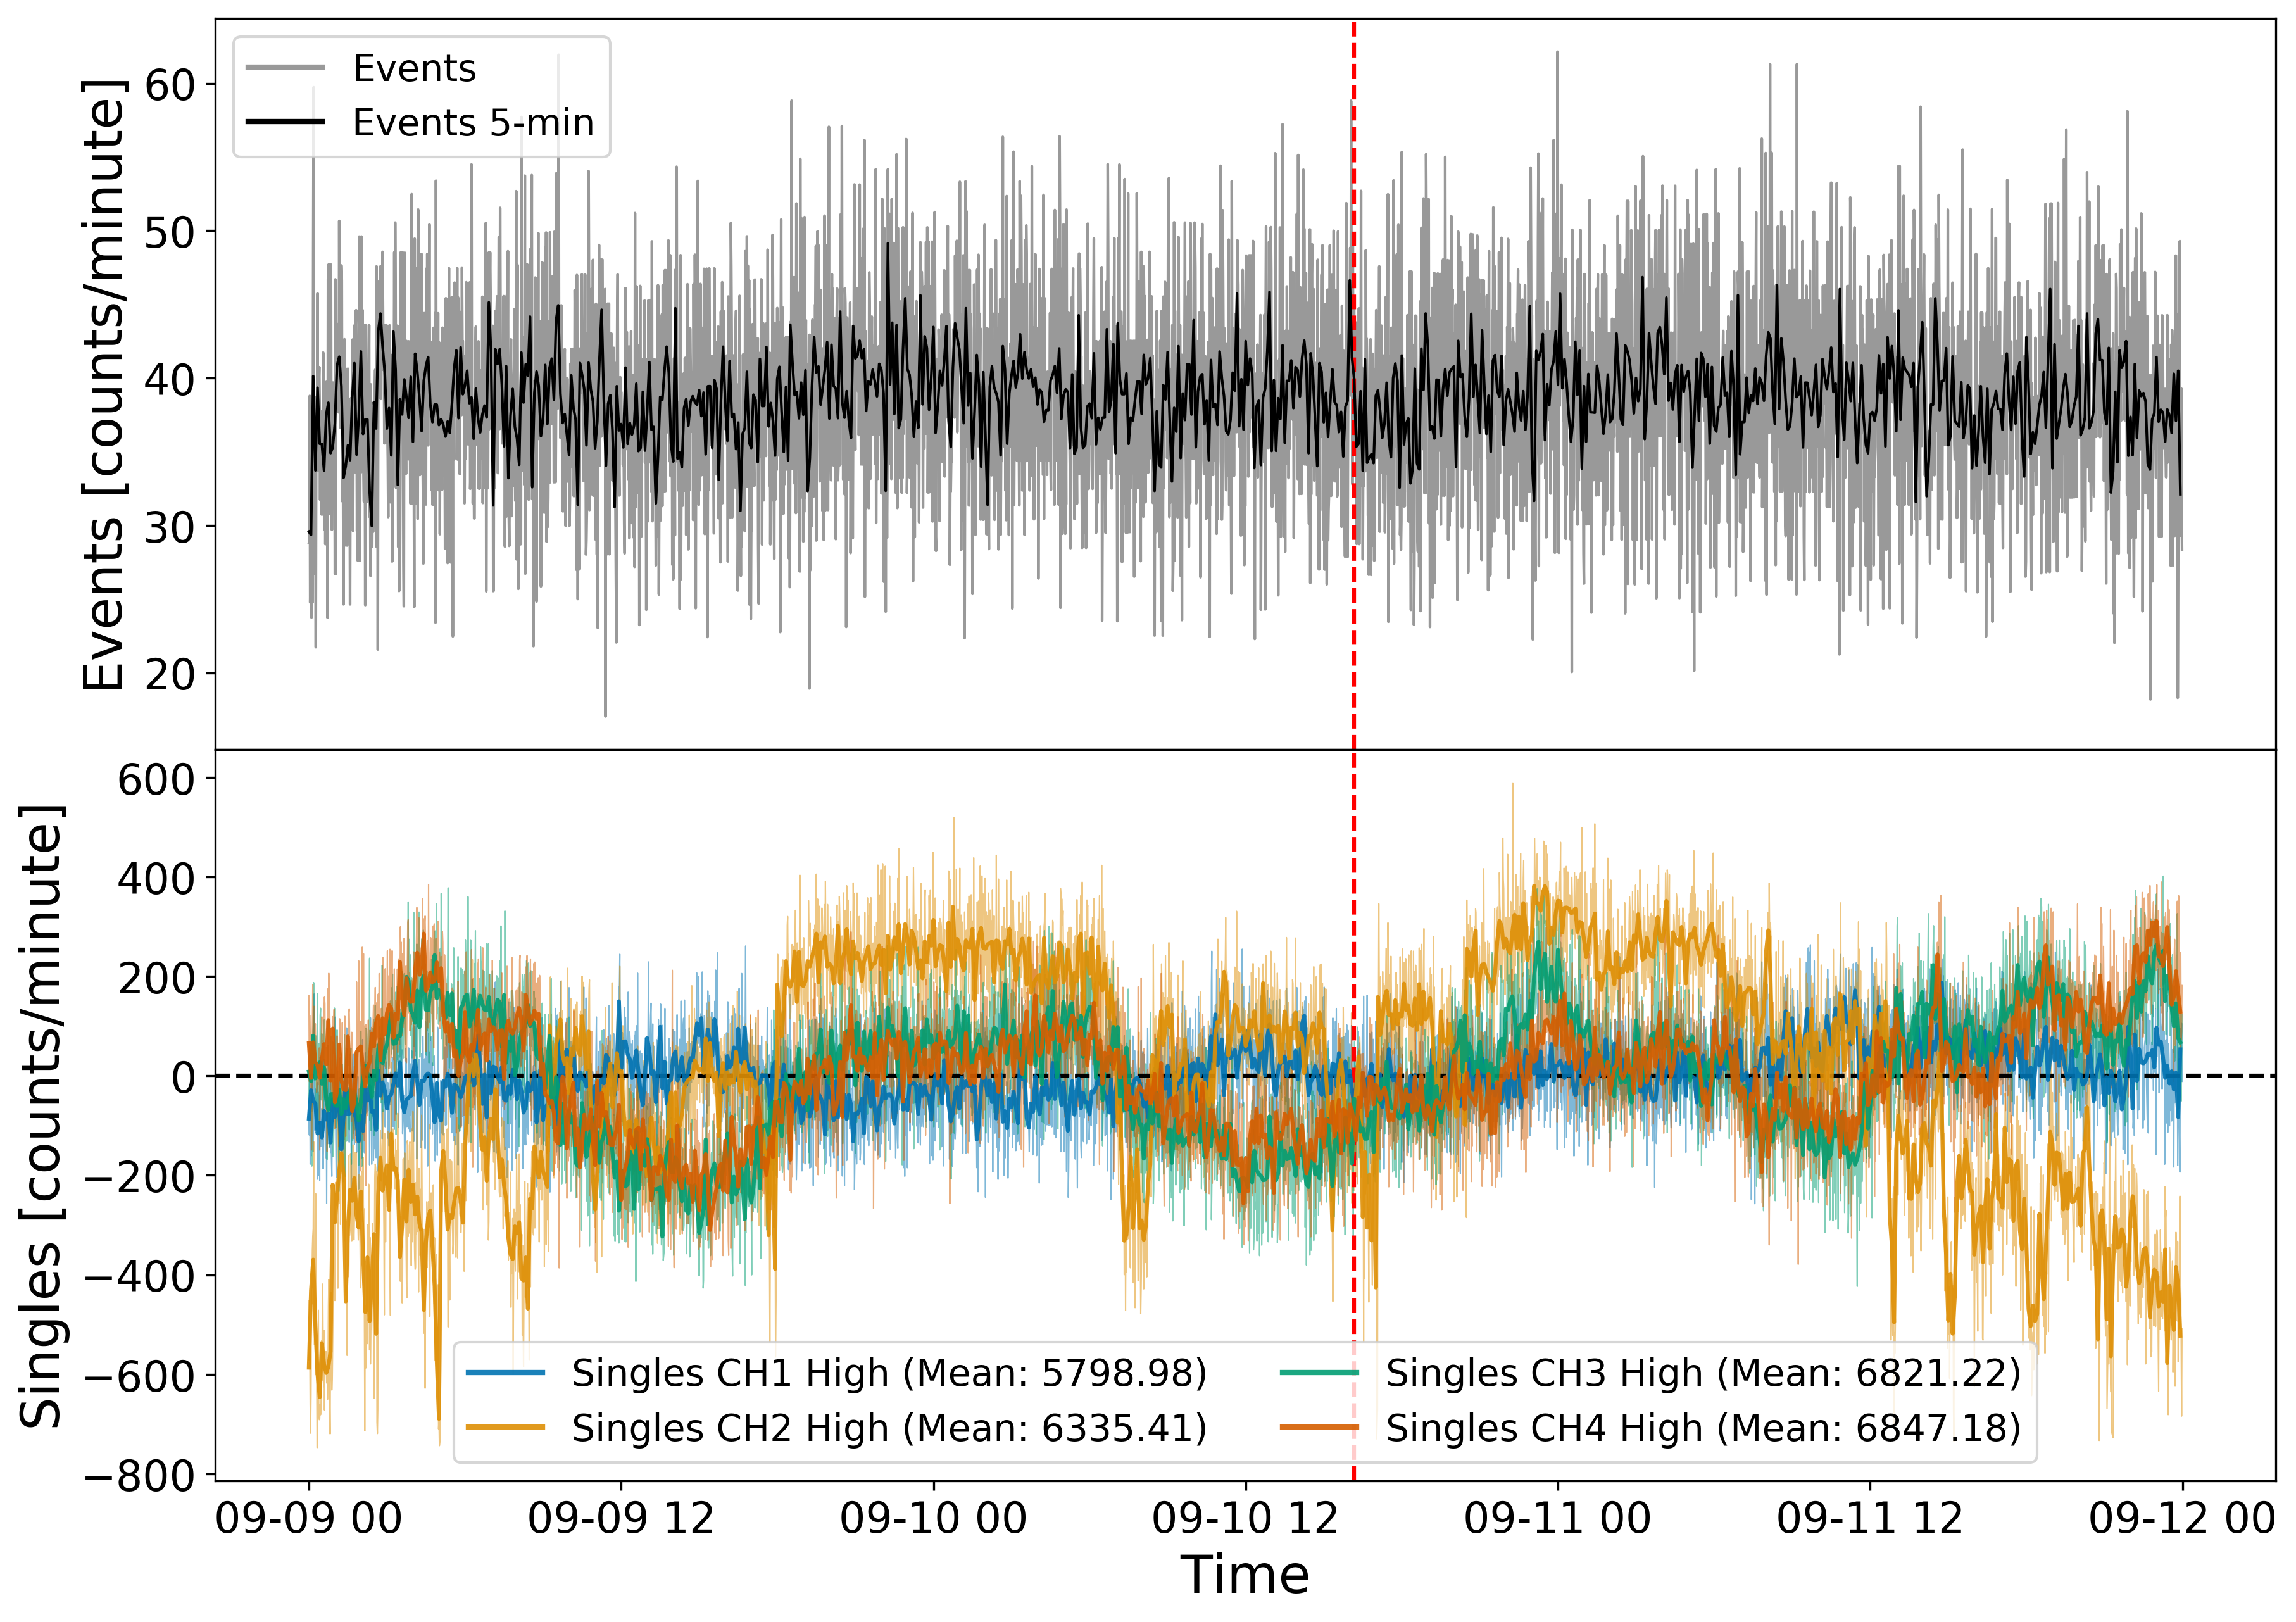
\includegraphics[width=0.48\columnwidth]{GLE72_501_Pcorr.png}
		\label{fig:GLE72_501_Pcorr}}
	%\qquad
	\subfloat[HS 203 (College Hageveld)]{
		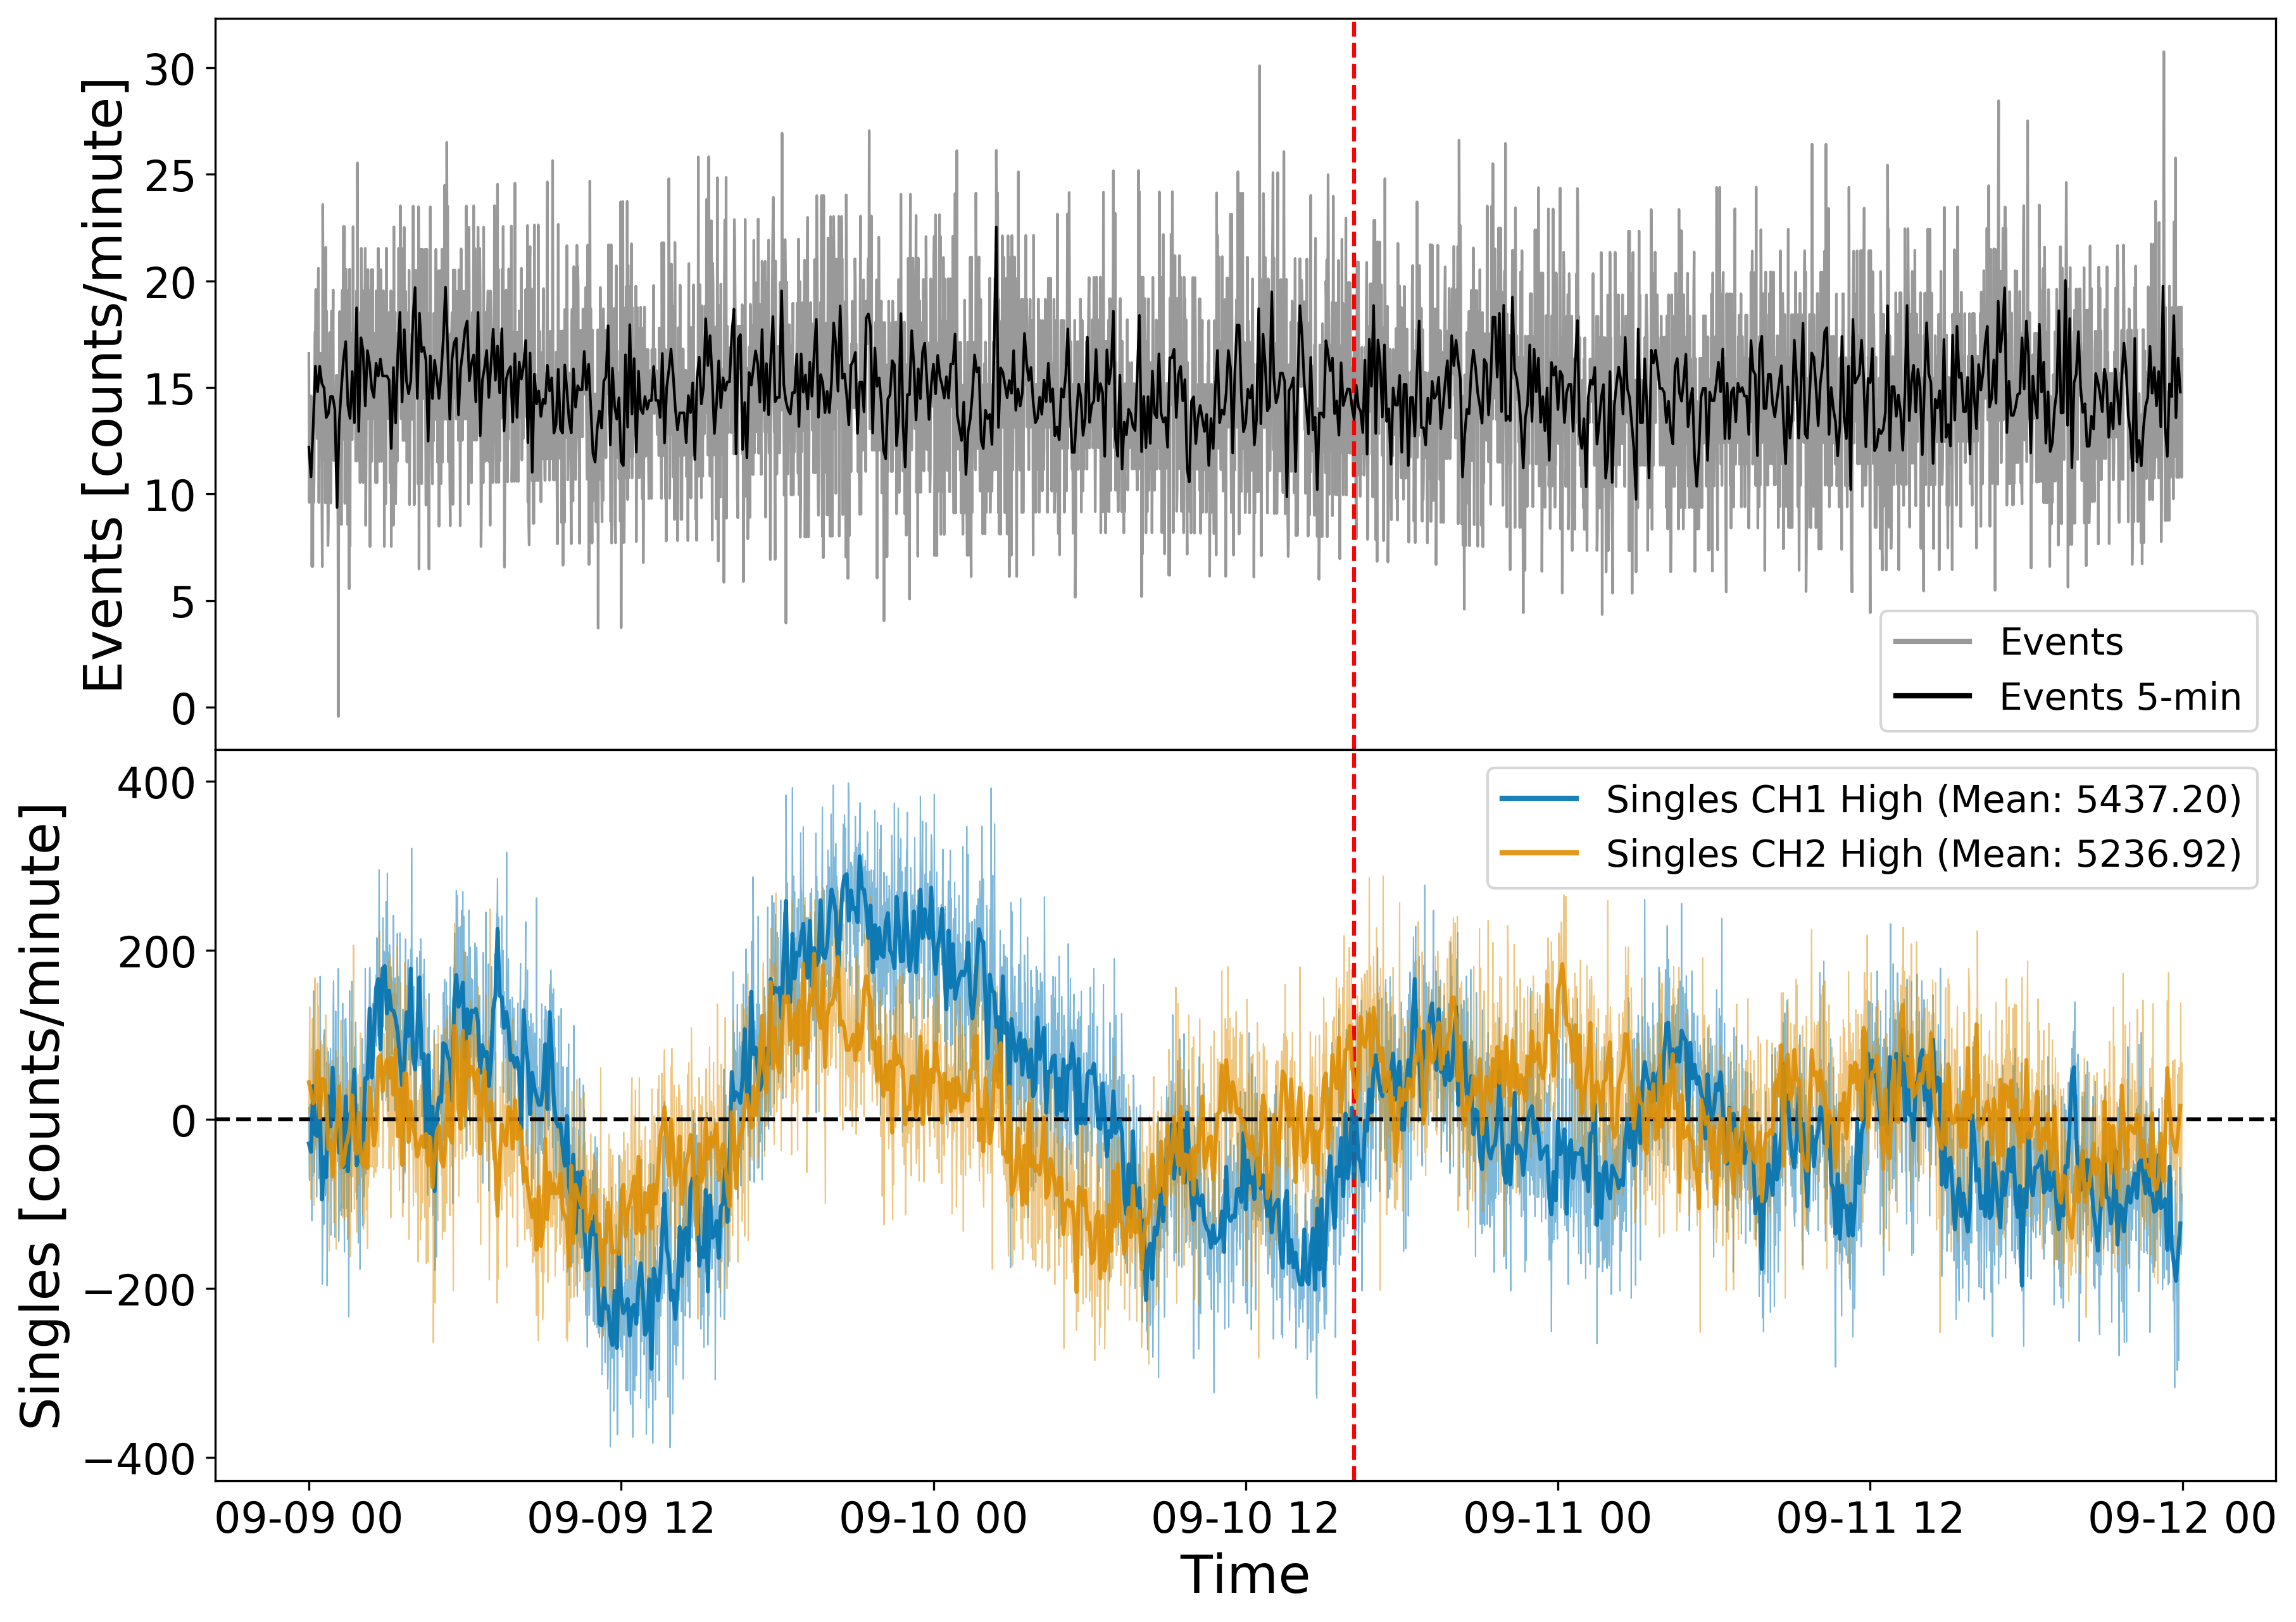
\includegraphics[width=0.48\columnwidth]{GLE72_203_Pcorr.png}
		\label{fig:GLE72_203_Pcorr}} \\
	
	
	\caption{Pressure corrected HiSPARC data for 2 stations around the epoch of GLE 72. The top panel of each subplot shows the minute-averaged trigger events between detectors within the station, while the bottom panel shows the mean-shifted, minute-averaged counts by each individual detector in the station. The vertical red, dashed line depicts the approximate onset time of the GLE.}
	\label{fig:GLE_72_Pcorr}
\end{figure}


%%%%%%%%%%%%%%%%%%%%%%%%%%%%%%%%%%%%%%%%%%%%%%%%%%%%%%%%%%%%%%%%%%%%%
\subsection{Pressure Corrected Observations of Forbush Decreases}



\begin{figure}[ht]
	\centering
	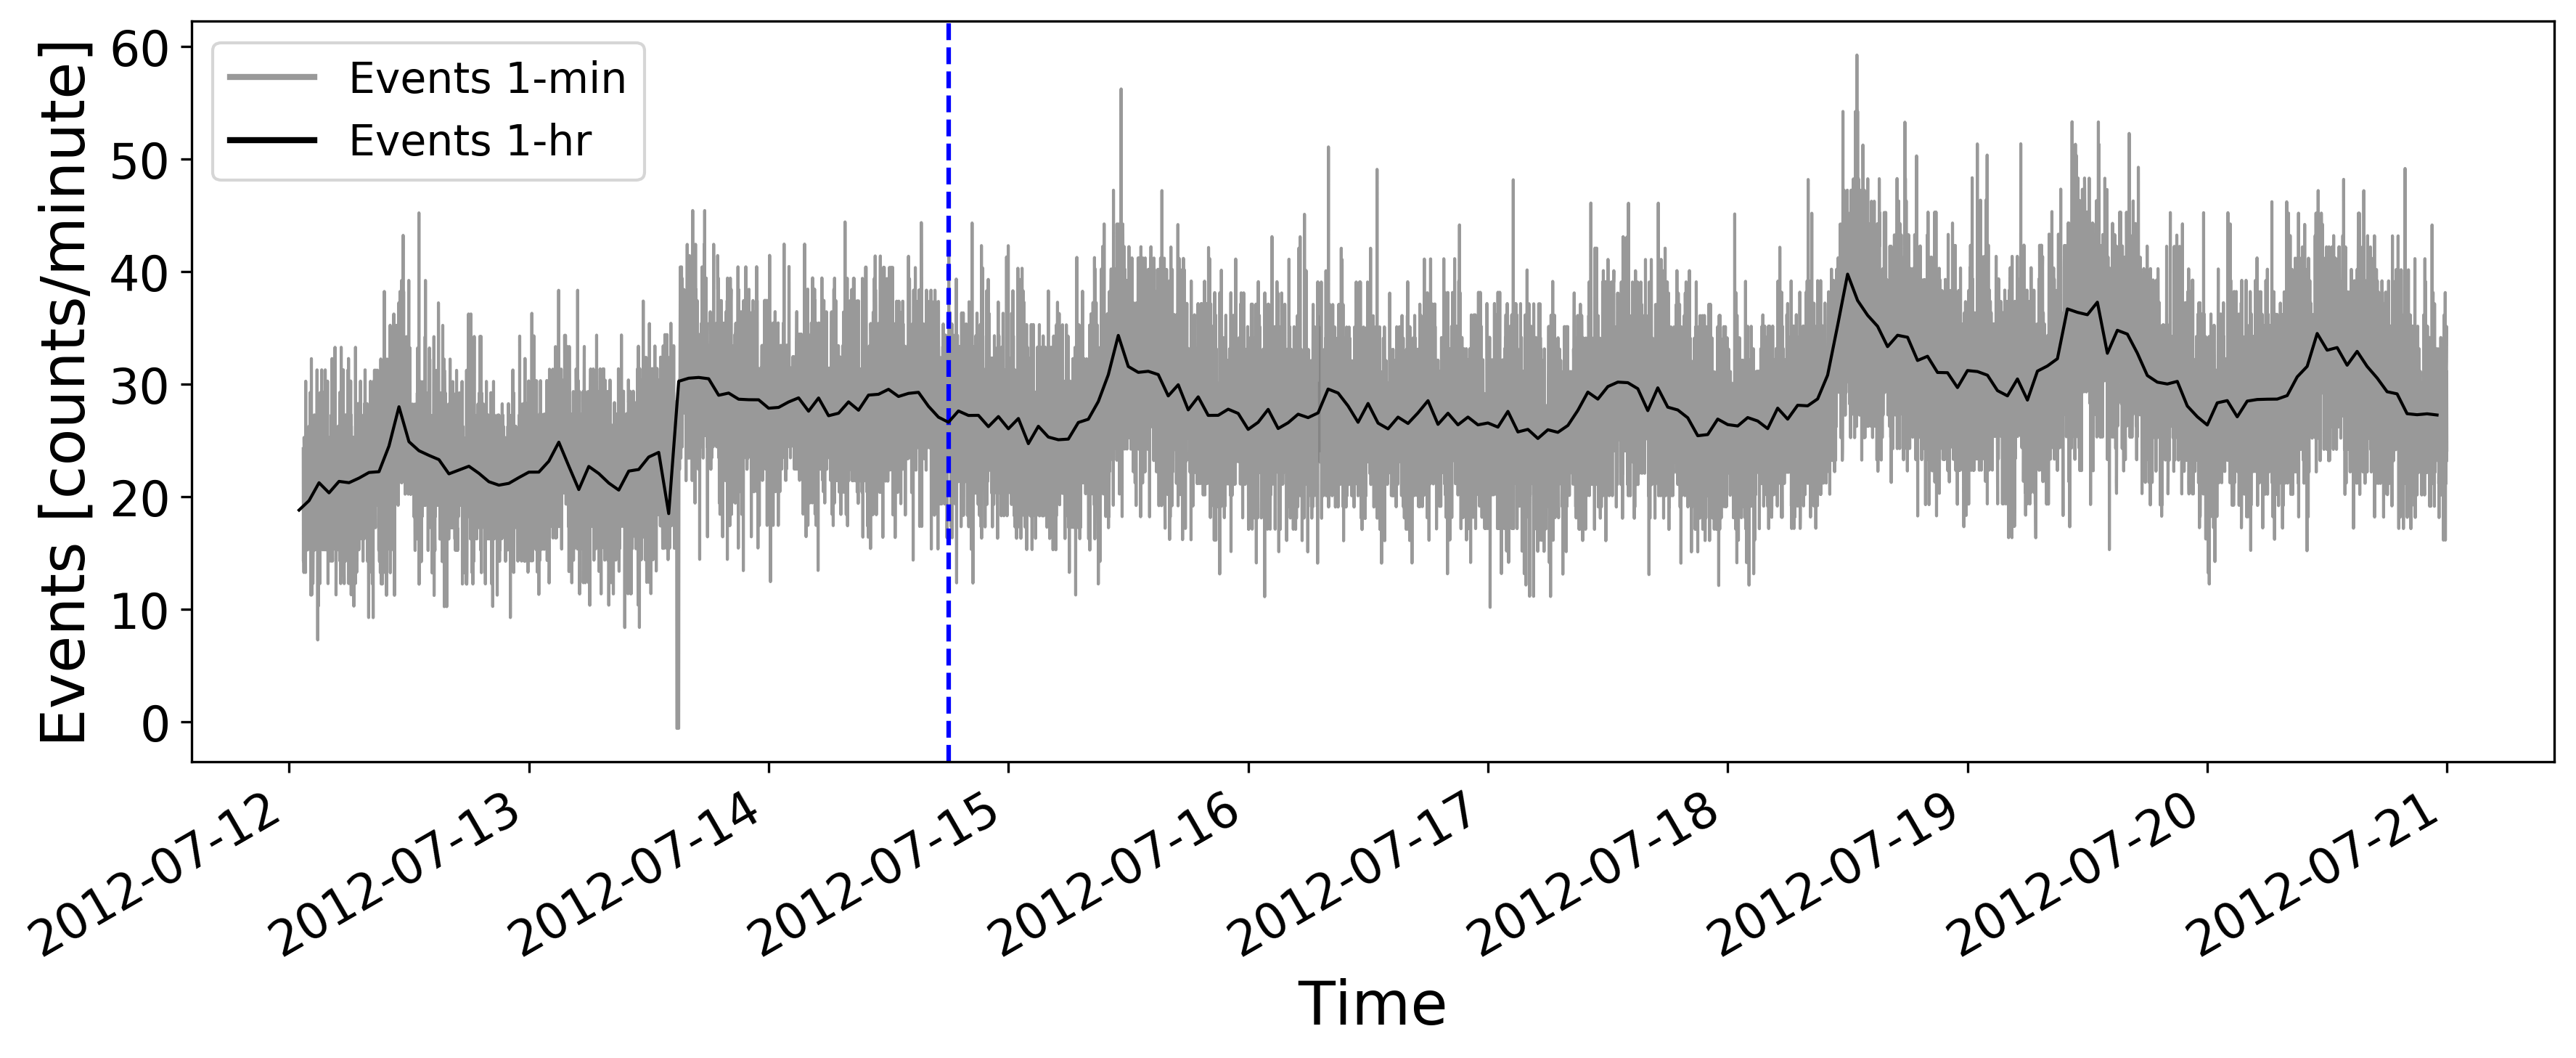
\includegraphics[width=0.65\columnwidth]{FD_201207_8001_Pcorr.png}
	\caption{...}
	\label{fig:FD_201207_8001_Pcorr}
\end{figure}



\begin{figure}[ht]
	\centering
	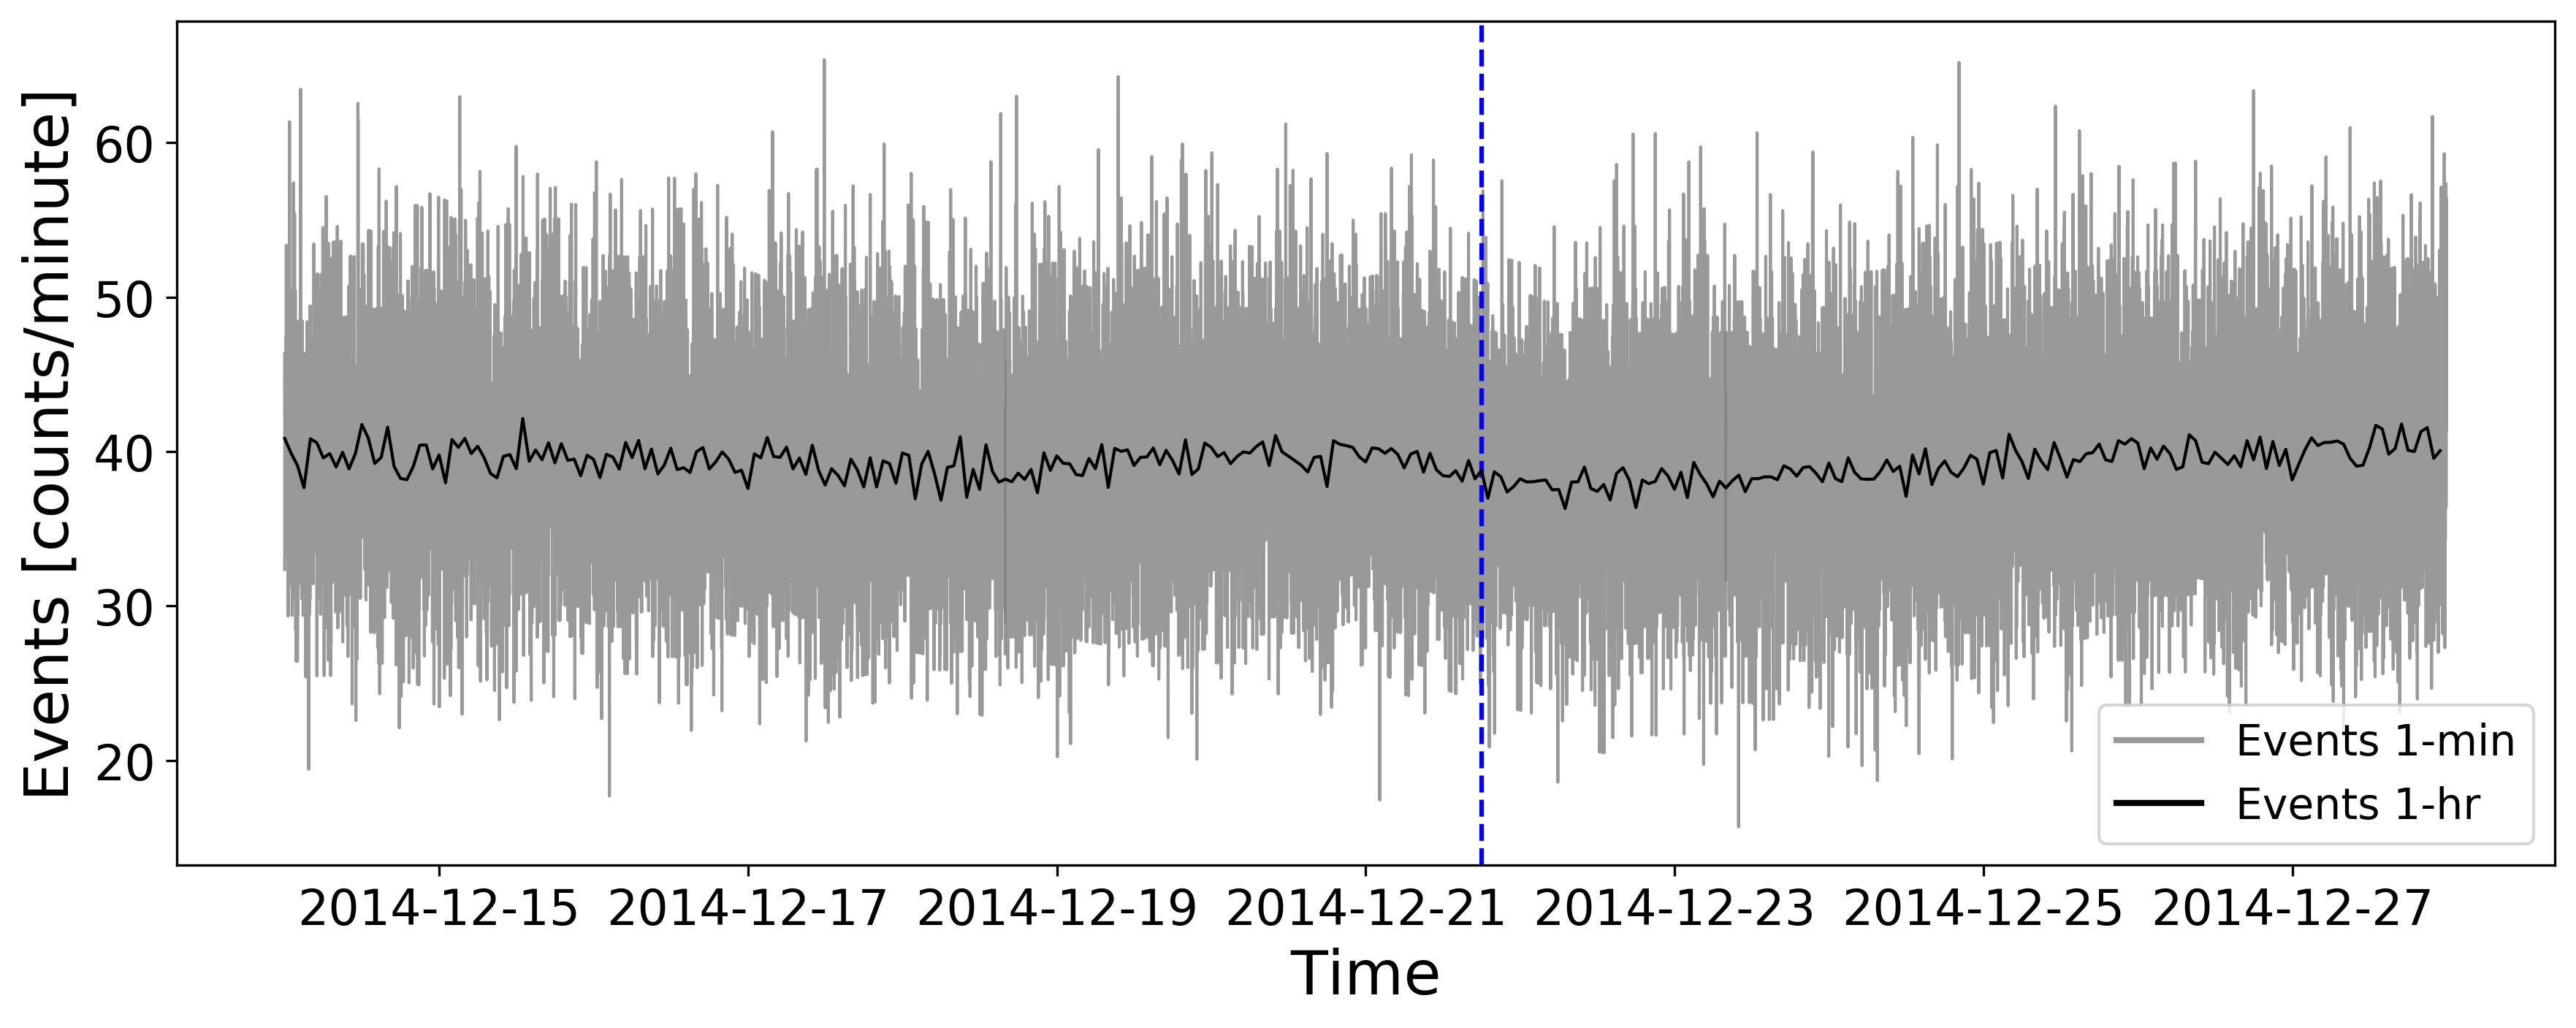
\includegraphics[width=0.65\columnwidth]{FD_201412_501_Pcorr.png}
	\caption{...}
	\label{fig:FD_201412_501_Pcorr}
\end{figure}



\begin{figure}[ht]
	\centering
	\subfloat[HS 501 (Nikhef)]{
		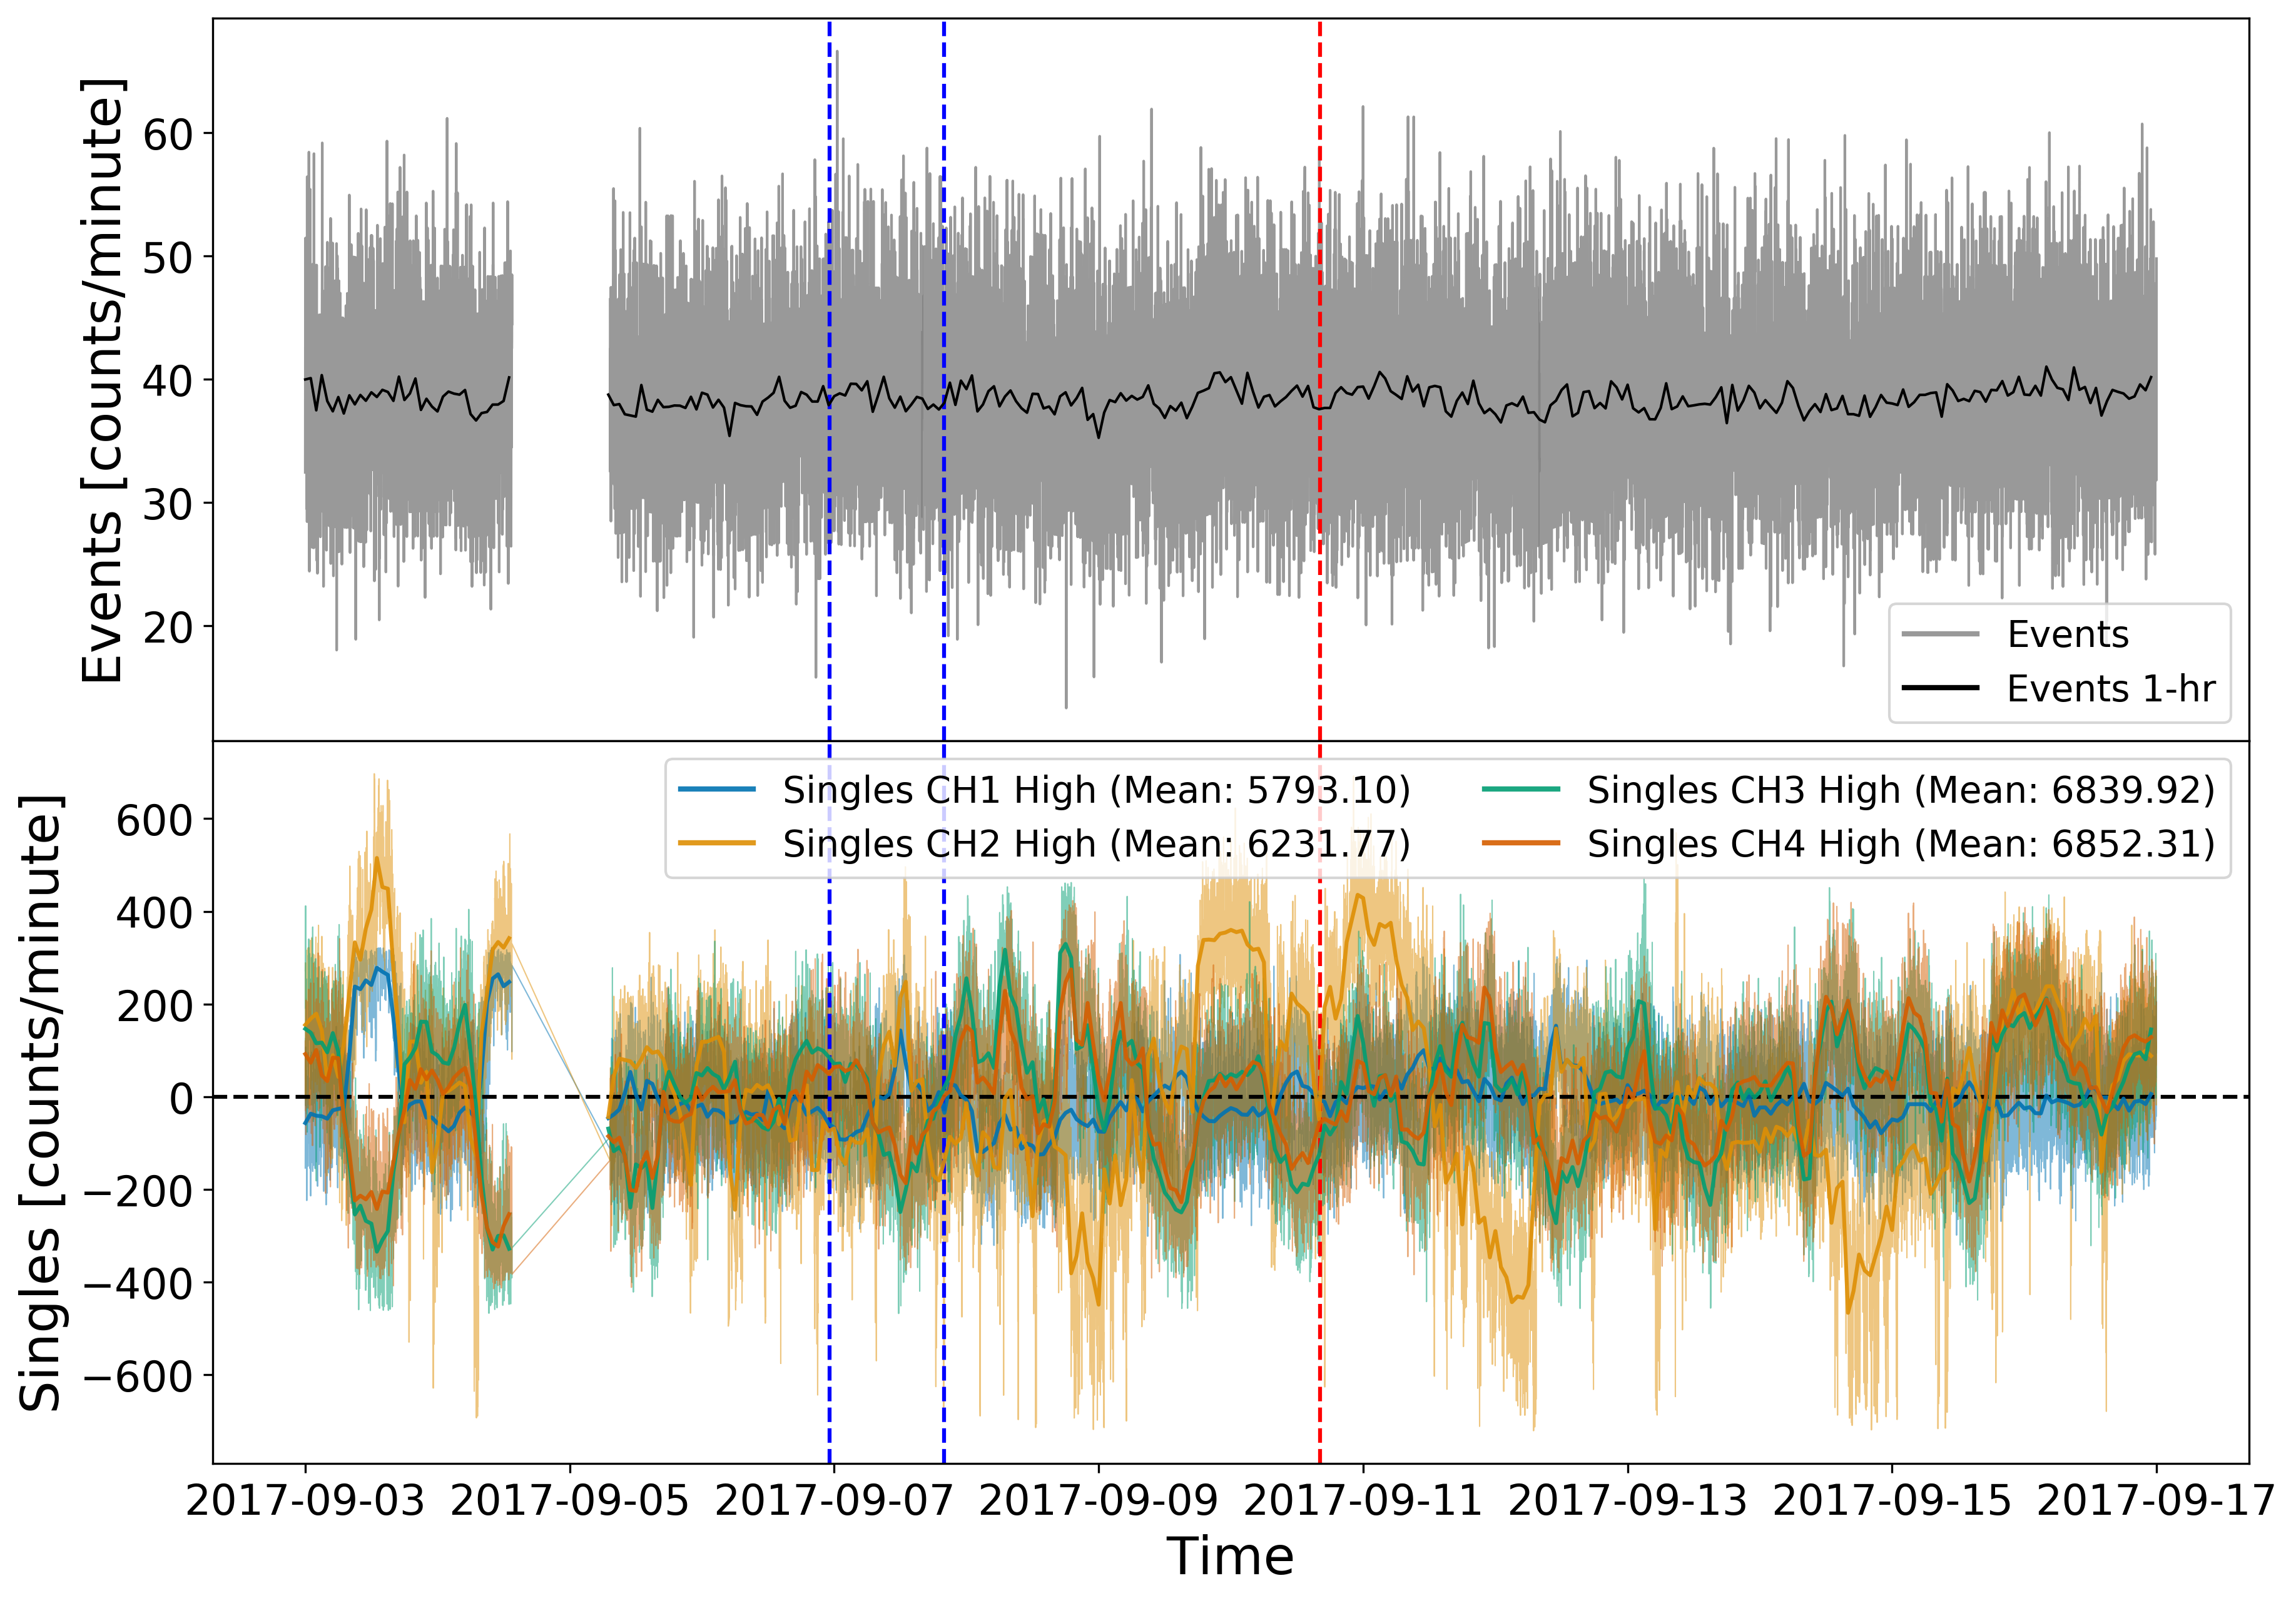
\includegraphics[width=0.48\columnwidth]{FD_GLE72_501_Pcorr.png}
		\label{fig:FD_GLE72_501_Pcorr}}
	%\qquad
	\subfloat[HS 203 (College Hageveld)]{
		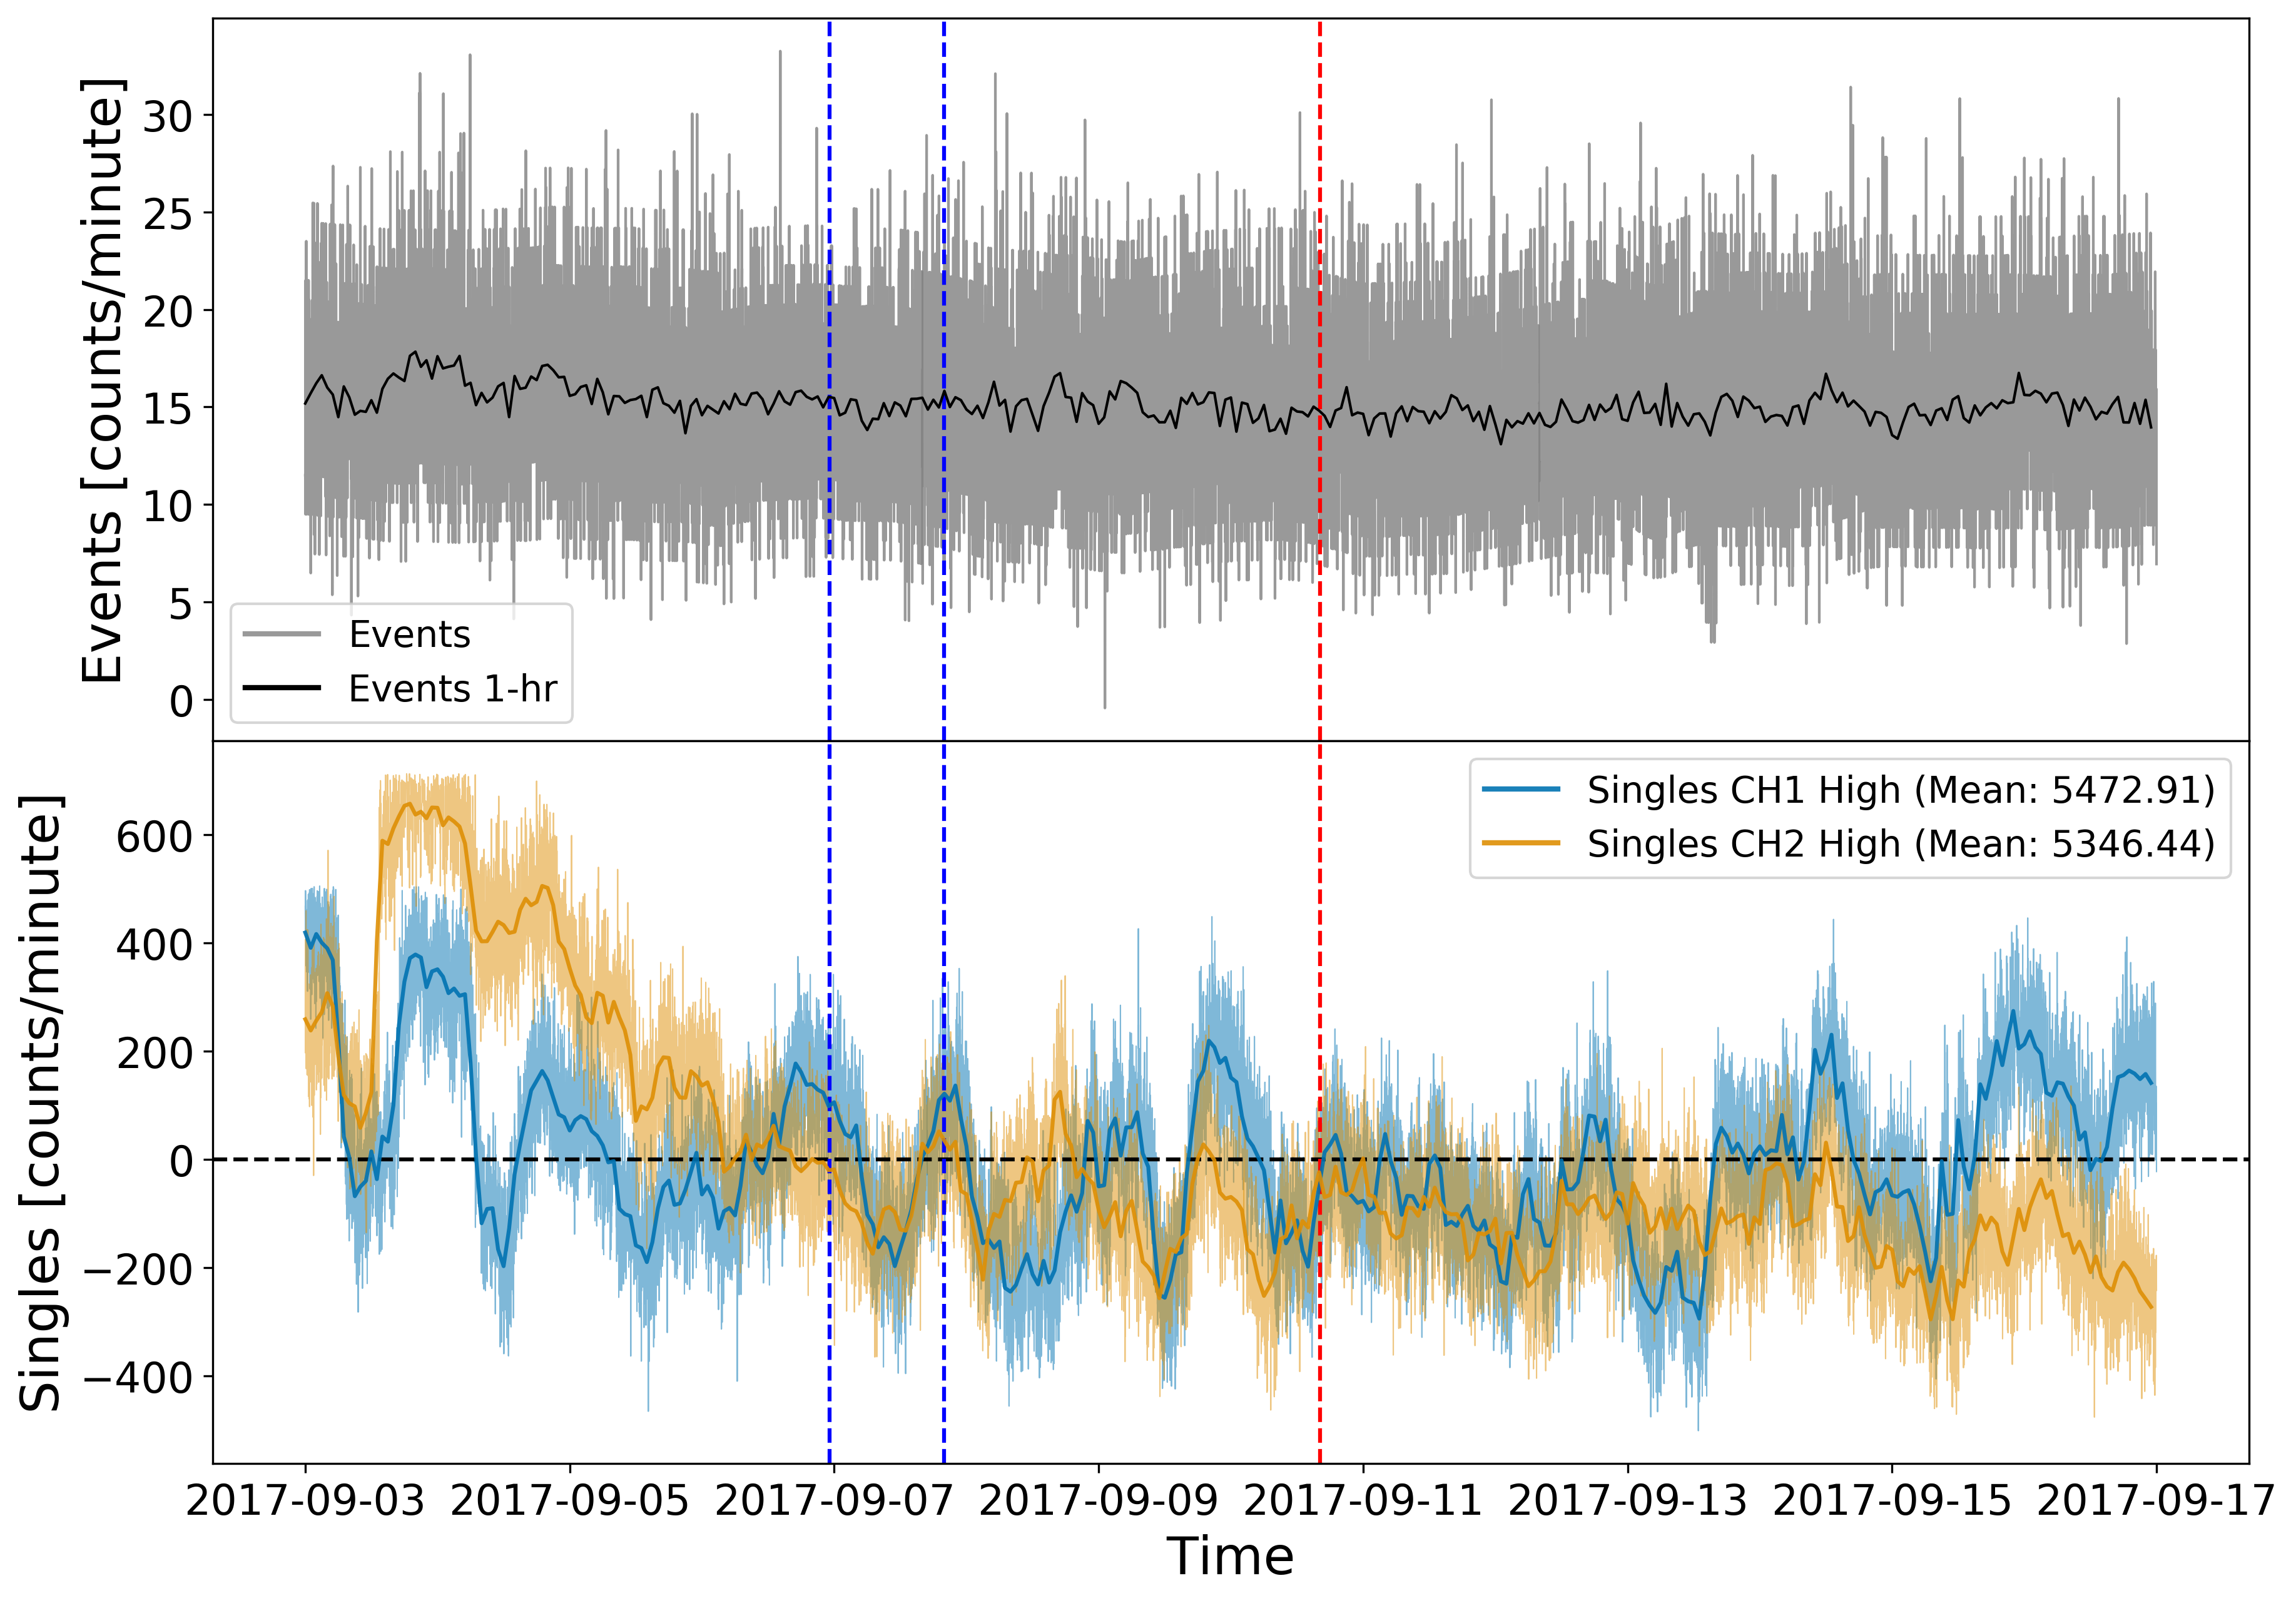
\includegraphics[width=0.48\columnwidth]{FD_GLE72_203_Pcorr.png}
		\label{fig:FD_GLE72_203_Pcorr}} \\
	
	
	\caption{Pressure corrected HiSPARC data for [n] stations around the epoch in which there were several FDs close to the onset of GLE 72. The top panel of each subplot shows the minute-averaged trigger events between detectors within the station, while the bottom panel shows the mean-shifted, minute-averaged counts by each individual detector in the station. The vertical blue-dashed lines show the approximate onset-times of the two FDs observed around this epoch and the red-dashed line depicts the approximate onset time of the GLE.}
	\label{fig:FD_GLE72_Pcorr}
\end{figure}



%%%%%%%%%%%%%%%%%%%%%%%%%%%%%%%%%%%%%%%%%%%%%%%%%%%%%%%%%%%%%%%%%%%%%
%%%%%%%%%%%%%%%%%%%%%%%%%%%%%%%%%%%%%%%%%%%%%%%%%%%%%%%%%%%%%%%%%%%%%
\section{Discussion}\label{sec:HS_discussion}

Throughout this chapter the feasibility of using the HiSPARC network of muon detectors has been analysed. This has involved performing cosmic ray air shower simluations using CORSIKA and performing backwards